% Options for packages loaded elsewhere
\PassOptionsToPackage{unicode}{hyperref}
\PassOptionsToPackage{hyphens}{url}
\PassOptionsToPackage{dvipsnames,svgnames,x11names}{xcolor}
%
\documentclass[
  11pt,
  a4paper,
]{book}

\usepackage{amsmath,amssymb}
\usepackage{lmodern}
\usepackage{iftex}
\ifPDFTeX
  \usepackage[T1]{fontenc}
  \usepackage[utf8]{inputenc}
  \usepackage{textcomp} % provide euro and other symbols
\else % if luatex or xetex
  \usepackage{unicode-math}
  \defaultfontfeatures{Scale=MatchLowercase}
  \defaultfontfeatures[\rmfamily]{Ligatures=TeX,Scale=1}
\fi
% Use upquote if available, for straight quotes in verbatim environments
\IfFileExists{upquote.sty}{\usepackage{upquote}}{}
\IfFileExists{microtype.sty}{% use microtype if available
  \usepackage[]{microtype}
  \UseMicrotypeSet[protrusion]{basicmath} % disable protrusion for tt fonts
}{}
\makeatletter
\@ifundefined{KOMAClassName}{% if non-KOMA class
  \IfFileExists{parskip.sty}{%
    \usepackage{parskip}
  }{% else
    \setlength{\parindent}{0pt}
    \setlength{\parskip}{6pt plus 2pt minus 1pt}}
}{% if KOMA class
  \KOMAoptions{parskip=half}}
\makeatother
\usepackage{xcolor}
\setlength{\emergencystretch}{3em} % prevent overfull lines
\setcounter{secnumdepth}{5}
% Make \paragraph and \subparagraph free-standing
\ifx\paragraph\undefined\else
  \let\oldparagraph\paragraph
  \renewcommand{\paragraph}[1]{\oldparagraph{#1}\mbox{}}
\fi
\ifx\subparagraph\undefined\else
  \let\oldsubparagraph\subparagraph
  \renewcommand{\subparagraph}[1]{\oldsubparagraph{#1}\mbox{}}
\fi


\providecommand{\tightlist}{%
  \setlength{\itemsep}{0pt}\setlength{\parskip}{0pt}}\usepackage{longtable,booktabs,array}
\usepackage{calc} % for calculating minipage widths
% Correct order of tables after \paragraph or \subparagraph
\usepackage{etoolbox}
\makeatletter
\patchcmd\longtable{\par}{\if@noskipsec\mbox{}\fi\par}{}{}
\makeatother
% Allow footnotes in longtable head/foot
\IfFileExists{footnotehyper.sty}{\usepackage{footnotehyper}}{\usepackage{footnote}}
\makesavenoteenv{longtable}
\usepackage{graphicx}
\makeatletter
\def\maxwidth{\ifdim\Gin@nat@width>\linewidth\linewidth\else\Gin@nat@width\fi}
\def\maxheight{\ifdim\Gin@nat@height>\textheight\textheight\else\Gin@nat@height\fi}
\makeatother
% Scale images if necessary, so that they will not overflow the page
% margins by default, and it is still possible to overwrite the defaults
% using explicit options in \includegraphics[width, height, ...]{}
\setkeys{Gin}{width=\maxwidth,height=\maxheight,keepaspectratio}
% Set default figure placement to htbp
\makeatletter
\def\fps@figure{htbp}
\makeatother
\newlength{\cslhangindent}
\setlength{\cslhangindent}{1.5em}
\newlength{\csllabelwidth}
\setlength{\csllabelwidth}{3em}
\newlength{\cslentryspacingunit} % times entry-spacing
\setlength{\cslentryspacingunit}{\parskip}
\newenvironment{CSLReferences}[2] % #1 hanging-ident, #2 entry spacing
 {% don't indent paragraphs
  \setlength{\parindent}{0pt}
  % turn on hanging indent if param 1 is 1
  \ifodd #1
  \let\oldpar\par
  \def\par{\hangindent=\cslhangindent\oldpar}
  \fi
  % set entry spacing
  \setlength{\parskip}{#2\cslentryspacingunit}
 }%
 {}
\usepackage{calc}
\newcommand{\CSLBlock}[1]{#1\hfill\break}
\newcommand{\CSLLeftMargin}[1]{\parbox[t]{\csllabelwidth}{#1}}
\newcommand{\CSLRightInline}[1]{\parbox[t]{\linewidth - \csllabelwidth}{#1}\break}
\newcommand{\CSLIndent}[1]{\hspace{\cslhangindent}#1}

\usepackage{amsmath}
\usepackage{booktabs}
\usepackage{caption}
\usepackage{longtable}
\makeatletter
\@ifpackageloaded{tcolorbox}{}{\usepackage[many]{tcolorbox}}
\@ifpackageloaded{fontawesome5}{}{\usepackage{fontawesome5}}
\definecolor{quarto-callout-color}{HTML}{909090}
\definecolor{quarto-callout-note-color}{HTML}{0758E5}
\definecolor{quarto-callout-important-color}{HTML}{CC1914}
\definecolor{quarto-callout-warning-color}{HTML}{EB9113}
\definecolor{quarto-callout-tip-color}{HTML}{00A047}
\definecolor{quarto-callout-caution-color}{HTML}{FC5300}
\definecolor{quarto-callout-color-frame}{HTML}{acacac}
\definecolor{quarto-callout-note-color-frame}{HTML}{4582ec}
\definecolor{quarto-callout-important-color-frame}{HTML}{d9534f}
\definecolor{quarto-callout-warning-color-frame}{HTML}{f0ad4e}
\definecolor{quarto-callout-tip-color-frame}{HTML}{02b875}
\definecolor{quarto-callout-caution-color-frame}{HTML}{fd7e14}
\makeatother
\makeatletter
\makeatother
\makeatletter
\@ifpackageloaded{bookmark}{}{\usepackage{bookmark}}
\makeatother
\makeatletter
\@ifpackageloaded{caption}{}{\usepackage{caption}}
\AtBeginDocument{%
\ifdefined\contentsname
  \renewcommand*\contentsname{Table of contents}
\else
  \newcommand\contentsname{Table of contents}
\fi
\ifdefined\listfigurename
  \renewcommand*\listfigurename{List of Figures}
\else
  \newcommand\listfigurename{List of Figures}
\fi
\ifdefined\listtablename
  \renewcommand*\listtablename{List of Tables}
\else
  \newcommand\listtablename{List of Tables}
\fi
\ifdefined\figurename
  \renewcommand*\figurename{Figure}
\else
  \newcommand\figurename{Figure}
\fi
\ifdefined\tablename
  \renewcommand*\tablename{Table}
\else
  \newcommand\tablename{Table}
\fi
}
\@ifpackageloaded{float}{}{\usepackage{float}}
\floatstyle{ruled}
\@ifundefined{c@chapter}{\newfloat{codelisting}{h}{lop}}{\newfloat{codelisting}{h}{lop}[chapter]}
\floatname{codelisting}{Listing}
\newcommand*\listoflistings{\listof{codelisting}{List of Listings}}
\makeatother
\makeatletter
\@ifpackageloaded{caption}{}{\usepackage{caption}}
\@ifpackageloaded{subcaption}{}{\usepackage{subcaption}}
\makeatother
\makeatletter
\@ifpackageloaded{tcolorbox}{}{\usepackage[many]{tcolorbox}}
\makeatother
\makeatletter
\@ifundefined{shadecolor}{\definecolor{shadecolor}{rgb}{.97, .97, .97}}
\makeatother
\makeatletter
\makeatother
\ifLuaTeX
  \usepackage{selnolig}  % disable illegal ligatures
\fi
\IfFileExists{bookmark.sty}{\usepackage{bookmark}}{\usepackage{hyperref}}
\IfFileExists{xurl.sty}{\usepackage{xurl}}{} % add URL line breaks if available
\urlstyle{same} % disable monospaced font for URLs
% Make links footnotes instead of hotlinks:
\DeclareRobustCommand{\href}[2]{#2\footnote{\url{#1}}}
\hypersetup{
  pdftitle={EUROCONTROL Standard Inputs for Economic Analyses},
  pdfauthor={EUROCONTROL Business Cases team},
  colorlinks=true,
  linkcolor={Maroon},
  filecolor={Maroon},
  citecolor={Blue},
  urlcolor={Blue},
  pdfcreator={LaTeX via pandoc}}

\title{EUROCONTROL Standard Inputs for Economic Analyses}
\author{EUROCONTROL Business Cases team}
\date{3/1/23}

\begin{document}
\frontmatter
\maketitle
\ifdefined\Shaded\renewenvironment{Shaded}{\begin{tcolorbox}[boxrule=0pt, sharp corners, interior hidden, frame hidden, borderline west={3pt}{0pt}{shadecolor}, enhanced, breakable]}{\end{tcolorbox}}\fi

\renewcommand*\contentsname{Table of contents}
{
\hypersetup{linkcolor=}
\setcounter{tocdepth}{2}
\tableofcontents
}
\mainmatter
\bookmarksetup{startatroot}

\hypertarget{about-us}{%
\chapter*{About us}\label{about-us}}
\addcontentsline{toc}{chapter}{About us}

\markboth{About us}{About us}

The EUROCONTROL Business Cases team is a dedicated team of experts that
support stakeholders who need to choose between different solutions and
alternatives, using the best available data. For 20 years, EUROCONTROL
has been providing ATM decision makers with a wide range of regularly
updated Standard Inputs to help them to take rational long-term
investment decision.

\bookmarksetup{startatroot}

\hypertarget{notice-and-disclaimer}{%
\chapter*{Notice and Disclaimer}\label{notice-and-disclaimer}}
\addcontentsline{toc}{chapter}{Notice and Disclaimer}

\markboth{Notice and Disclaimer}{Notice and Disclaimer}

The EUROCONTROL Business Cases team has made every effort to ensure that
the information and analysis contained in this document are as accurate
as possible. Only information from quoted sources has been used and
information relating to named parties has been checked with the parties
concerned. Despite these precautions, should you find any errors or
inconsistencies we would be grateful if you could please bring them to
our attention. Our email address is
\href{mailto:aviation.intelligence@eurocontrol.int}{\nolinkurl{aviation.intelligence@eurocontrol.int}}

This document is published by the EUROCONTROL Business Cases team in the
interest of the exchange of information.

Information contained in this document may not be modified without prior
written permission from the EUROCONTROL Business Cases team.

The views expressed herein do not necessarily respect the official views
or policy of EUROCONTROL, which makes no warranty, either implied or
express, for the information contained in this document, neither does it
assume any legal liability or responsibility for the accuracy,
completeness or usefulness of this information.

\hypertarget{publications}{%
\section*{Publications}\label{publications}}
\addcontentsline{toc}{section}{Publications}

\markright{Publications}

EUROCONTROL Headquarters\\
96 Rue de la Fusée\\
B-1130 BRUSSELS\\
Tel: +32 (0)2 729 1152\\
Fax: +32 (0)2 729 5149\\
E-mail: publications@eurocontrol.int

\bookmarksetup{startatroot}

\hypertarget{foreword}{%
\chapter*{Foreword}\label{foreword}}
\addcontentsline{toc}{chapter}{Foreword}

\markboth{Foreword}{Foreword}

The first version of the Standard Inputs for EUROCONTROL Economic
Analyses series was launched in 2002 and has been kept alive for 20
years now, with the dedication of several colleagues, in particular
Paula and Desirée who put a lot of effort to this document. Today we
take a new step and are launching the latest edition on an online
platform to allow for timely and continuous updates of the values,
following the pace of change in the aviation world.

Our first launch includes a selection of six values, complemented with
some general information and the remaining inputs will be updated over
the coming months. You can access the previous edition for the values
that are not yet updated through a link in each of the value sections.

\hypertarget{acknowledgements}{%
\section*{Acknowledgements}\label{acknowledgements}}
\addcontentsline{toc}{section}{Acknowledgements}

\markright{Acknowledgements}

We would like to show our gratitude to the many different colleagues
that have contributed to this endeavour by helping us develop the values
and get them online. Trying to name them would be impossible.

We have received valuable remarks and suggestions from all stakeholders
in the aviation value chain. In particular we have benefited from
stakeholders involved in the entire development life cycle, from ideas
to a working system. We strongly believe that this collaboration makes
the EUROCONTROL Standard Inputs for Economic Analyses a robust and
authoritative product.

Thank you all for making us learn every day!

\bookmarksetup{startatroot}

\hypertarget{introduction}{%
\chapter*{Introduction}\label{introduction}}
\addcontentsline{toc}{chapter}{Introduction}

\markboth{Introduction}{Introduction}

This document provides a set of data commonly used in economic and
financial analyses and appraisals, particulary in the field of ATM.

The aim of this document is to standardise the data used in the
different ATM-related assessments, facilitate the data access for the
different stakeholders involved and contribute to the comparability of
different analyses through relying on the same data.

In this edition (10.0.2):

\begin{itemize}
\tightlist
\item
  A selection of values has been updated according to the latest data
  available and published on the web:

  \begin{itemize}
  \tightlist
  \item
    \protect\hyperlink{sec-conversions}{General parameters}
  \item
    \protect\hyperlink{sec-geographical-areas}{Geographical areas}
  \item
    Chapter~\ref{sec-air-traffic-statistics-and-forecasts}
    \protect\hyperlink{sec-air-traffic-statistics-and-forecasts}{Air
    traffic statistics and forecast}
  \item
    Chapter~\ref{sec-number-of-ifr-flights}
    \protect\hyperlink{sec-number-of-ifr-flights}{Number of IFR flights}
  \item
    Chapter~\ref{sec-air-traffic-delay}
    \protect\hyperlink{sec-air-traffic-delay}{Air traffic delay}
  \item
    Chapter~\ref{sec-average-number-of-passengers}
    \protect\hyperlink{sec-average-number-of-passengers}{Average number
    of passengers}
  \end{itemize}
\item
  Two new values have been introduced:

  \begin{itemize}
  \tightlist
  \item
    Chapter~\ref{sec-shadow-cost-of-carbon}
    \protect\hyperlink{sec-shadow-cost-of-carbon}{Shadow cost of carbon}
  \item
    Chapter~\ref{sec-proportion-of-saf}
    \protect\hyperlink{sec-proportion-of-saf}{Proportion of Sustainable
    Aviation Fuel}
  \end{itemize}
\end{itemize}

Please note that the standard inputs have been compiled from EUROCONTROL
data and intelligence, from values provided by airspace users, ANSPs,
airports, IATA, EASA and other organisations, and from other relevant
documents which are publicly available.

They are average values and may not be appropriate in all circumstances.
The document also gives details of the sources of information, and
discusses the applicability and use of the values.

This document will remain a living document, and so comments and
suggestions are very welcome. Readers are invited to send these to
\href{mailto:aviation.intelligence@eurocontrol.int}{\nolinkurl{aviation.intelligence@eurocontrol.int}}.

\hypertarget{details-per-data-item}{%
\section*{Details per data item}\label{details-per-data-item}}

\markright{Details per data item}

For each standard input, the following information is provided, where
relevant.

\begin{longtable}[]{@{}
  >{\raggedright\arraybackslash}p{(\columnwidth - 2\tabcolsep) * \real{0.3333}}
  >{\raggedright\arraybackslash}p{(\columnwidth - 2\tabcolsep) * \real{0.6667}}@{}}
\toprule()
\begin{minipage}[b]{\linewidth}\raggedright
Section
\end{minipage} & \begin{minipage}[b]{\linewidth}\raggedright
Description
\end{minipage} \\
\midrule()
\endhead
EUROCONTROL recommended values & One or a set of recommended values put
forward by EUROCONTROL for the specific indicator. \\
Description & Any relevant information or details regarding the
recommended value (e.g.~information on how the value was computed, the
limitations on using the value, or other remarks). \\
When to use the input? & A recommendation on when and where the specific
input can be beneficial is provided here. \\
Comments & Any questions or further comments regarding the source or
derivation of the value, for example the degree of confidence in the
values and sources cited. \\
Related inputs & A link to other related standard inputs included in the
document. \\
References & A list of sources used for the specific input. \\
\bottomrule()
\end{longtable}

\bookmarksetup{startatroot}

\hypertarget{sec-conversions}{%
\chapter*{General parameters}\label{sec-conversions}}
\addcontentsline{toc}{chapter}{General parameters}

\markboth{General parameters}{General parameters}

Below are presented some key values used in the Standard Inputs and that
can serve as a reference for other uses.

\hypertarget{inflation}{%
\section*{Inflation}\label{inflation}}
\addcontentsline{toc}{section}{Inflation}

\markright{Inflation}

The inflation levels have been calculated based on the Harmonised Index
of Consumer Prices (HICP)
\protect\hyperlink{ref-eurostat:HICP}{{[}1{]}}, as the yearly difference
in the HICP. The HICP data was extracted from
\href{http://ec.europa.eu/eurostat}{Eurostat} HICP - annual data
(average index and rate of change) database (prc\_hicp\_aind).The annual
change in the index is shown in Table~\ref{tbl-inflation-table}.

\hypertarget{tbl-inflation-table}{}
\begin{longtable}{ccc}
\caption{\label{tbl-inflation-table}Annual average inflation values }\tabularnewline

\toprule
Year & Index & Rate of change \\ 
\midrule
2022 & $118.80$ & $9.19\%$ \\ 
2021 & $108.80$ & $2.84\%$ \\ 
2020 & $105.80$ & $0.36\%$ \\ 
2019 & $105.42$ & $1.47\%$ \\ 
2018 & $103.89$ & $1.89\%$ \\ 
2017 & $101.96$ & $1.71\%$ \\ 
2016 & $100.25$ & $0.25\%$ \\ 
2015 & $100.00$ & $0.10\%$ \\ 
2014 & $99.90$ & $0.55\%$ \\ 
2013 & $99.35$ & $1.50\%$ \\ 
2012 & $97.88$ & $2.64\%$ \\ 
2011 & $95.36$ & $3.10\%$ \\ 
2010 & $92.49$ & $2.09\%$ \\ 
2009 & $90.60$ & $0.98\%$ \\ 
2008 & $89.72$ & $3.54\%$ \\ 
2007 & $86.65$ & $2.34\%$ \\ 
2006 & $84.67$ & $2.20\%$ \\ 
2005 & $82.85$ & $2.17\%$ \\ 
2004 & $81.09$ & $2.01\%$ \\ 
2003 & $79.49$ & $1.96\%$ \\ 
2002 & $77.96$ & $2.08\%$ \\ 
2001 & $76.37$ & $2.19\%$ \\ 
2000 & $74.73$ & $1.90\%$ \\ 
\bottomrule
\end{longtable}

\hypertarget{exchange-rates}{%
\section*{Exchange Rate Conversion}\label{exchange-rates}}
\addcontentsline{toc}{section}{Exchange Rate Conversion}

\markright{Exchange Rate Conversion}

The currency exchange rates provided below are based on the European
Central Bank (ECB) rates that are published daily
\protect\hyperlink{ref-ECB:exchange_rates}{{[}2{]}}. The rates shown in
the table below correspond to the average rate for the year 2021 as
published by ECB.

\hypertarget{tbl-eurostat-exchange-rates}{}
\begin{longtable}{lcc}
\caption{\label{tbl-eurostat-exchange-rates}Average euro foreign exchange rate (2021) }\tabularnewline

\toprule
Currency & Currency-€ & €-Currency \\ 
\midrule
USD & 0.89 & 1.12 \\ 
GBP & 1.22 & 0.82 \\ 
\bottomrule
\end{longtable}

\hypertarget{cost-of-fuel}{%
\section*{Cost of fuel}\label{cost-of-fuel}}
\addcontentsline{toc}{section}{Cost of fuel}

\markright{Cost of fuel}

The cost of fuel used in this document is based on the 2021 average jet
fuel price handled by IATA
\protect\hyperlink{ref-iata:JetFuelPrice}{{[}3{]}}, unless otherwise
specified. All conversions are done using the values specified on this
page.

\hypertarget{tbl-cost-of-fuel}{}
\begin{longtable}{lccc}
\caption{\label{tbl-cost-of-fuel}Average jet fuel price }\tabularnewline

\toprule
Currency & Price per barrel & Price per gallon & Price per kg \\ 
\midrule
USD & 141.7 & 3.8 & 1.1 \\ 
EUR & 138.9 & 3.3 & 1.1 \\ 
\bottomrule
\end{longtable}

\hypertarget{conversion-values}{%
\section*{Conversion values}\label{conversion-values}}
\addcontentsline{toc}{section}{Conversion values}

\markright{Conversion values}

\hypertarget{tbl-conversion-values}{}
\begin{longtable}{ll}
\caption{\label{tbl-conversion-values}Units conversion values }\tabularnewline

\toprule
From & To \\ 
\midrule
1 nautical mile (NM) & 1.852 km \\ 
1 kilometre (km) & 0.53996 NM \\ 
1 tonne (metric = 1 000 kg) of jet fuel & 325.33 US gallons \\ 
 & 1 235 litres \\ 
 & 7.8 barrels \\ 
1 barrel (bbl) of jet fuel & 42 US gallons \\ 
 & 158.99 litres \\ 
 & 0.1291 tonne = 129.10 kg \\ 
1 US gallon of jet fuel (US gal) & 3.7854 litres \\ 
 & 3.073 kg \\ 
 & 6.7764 lb \\ 
Density of kerosene & 0.812 kg/litre \\ 
1 litre of fuel (l) & 0.26417 US gallons \\ 
1 kilogramme of fuel (kg) & 2.2046 lb \\ 
1 pound of fuel (lb) & 0.45359 kg \\ 
\bottomrule
\end{longtable}

\hypertarget{references}{%
\section*{References}\label{references}}
\addcontentsline{toc}{section}{References}

\markright{References}

\bookmarksetup{startatroot}

\hypertarget{sec-geographical-areas}{%
\chapter*{Geographical Areas}\label{sec-geographical-areas}}
\addcontentsline{toc}{chapter}{Geographical Areas}

\markboth{Geographical Areas}{Geographical Areas}

\hypertarget{member-states-and-geographical-areas-covered}{%
\section*{Member States and geographical areas
covered}\label{member-states-and-geographical-areas-covered}}
\addcontentsline{toc}{section}{Member States and geographical areas
covered}

\markright{Member States and geographical areas covered}

Single European Sky initiative and the European Civil Aviation
Conference (ECAC) are the different scopes that are covered in Standard
Inputs document.

\begin{figure}

{\centering 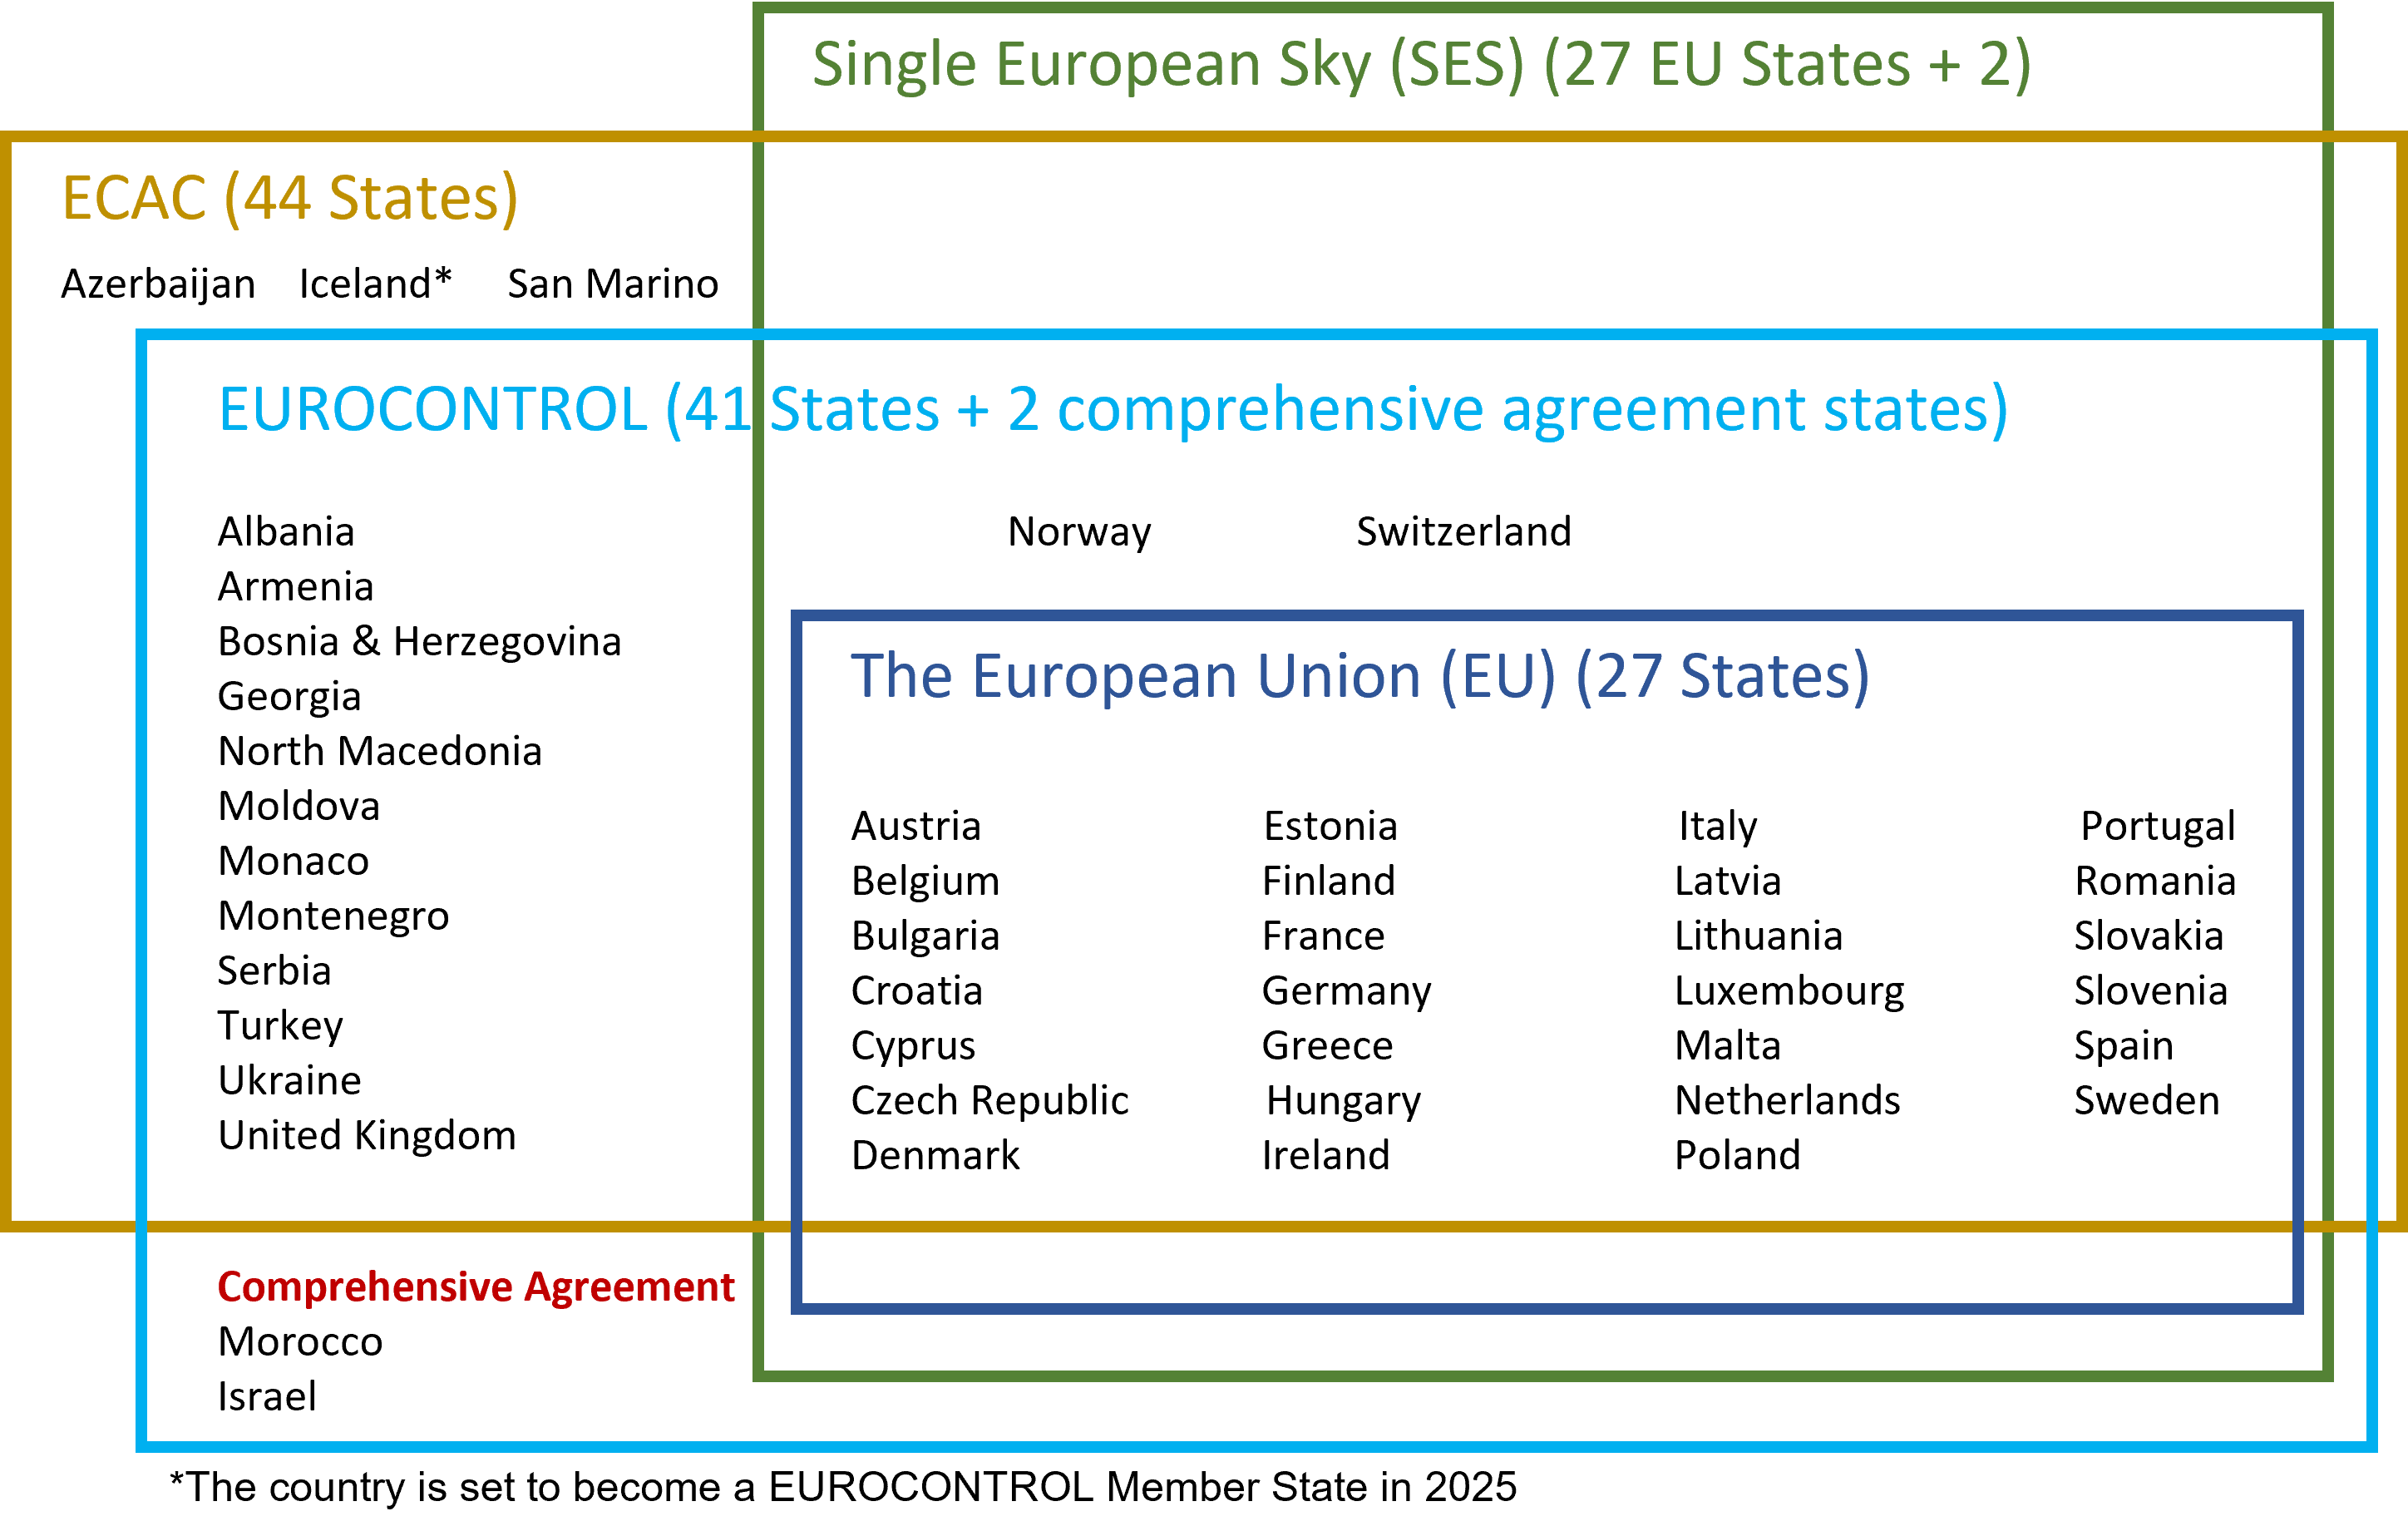
\includegraphics{./figures/eu_orgs.png}

}

\caption{\label{fig-member-states-set-diagram}State grouping}

\end{figure}

\hypertarget{eurocontrol-member-states}{%
\section*{EUROCONTROL Member States}\label{eurocontrol-member-states}}
\addcontentsline{toc}{section}{EUROCONTROL Member States}

\markright{EUROCONTROL Member States}

\begin{figure}

{\centering \includegraphics{./figures/eurocontrol_ms.png}

}

\caption{\label{fig-eurocontrol-member-states}EUROCONTROL Member States
(status: November 2020)}

\end{figure}

\hypertarget{airspace-of-the-ecac-member-states}{%
\section*{Airspace of the ECAC Member
States}\label{airspace-of-the-ecac-member-states}}
\addcontentsline{toc}{section}{Airspace of the ECAC Member States}

\markright{Airspace of the ECAC Member States}

ECAC is an intergovernmental organisation that was established by ICAO
and the Council of Europe. ECAC now has 44 Member States, including all
27 EU Member States, 31 of the 32 European Aviation Safety Agency Member
States, and all 41 EUROCONTROL Member States. The figure below is a
graphical representation of the airspace belonging to the ECAC states.

\begin{figure}

{\centering 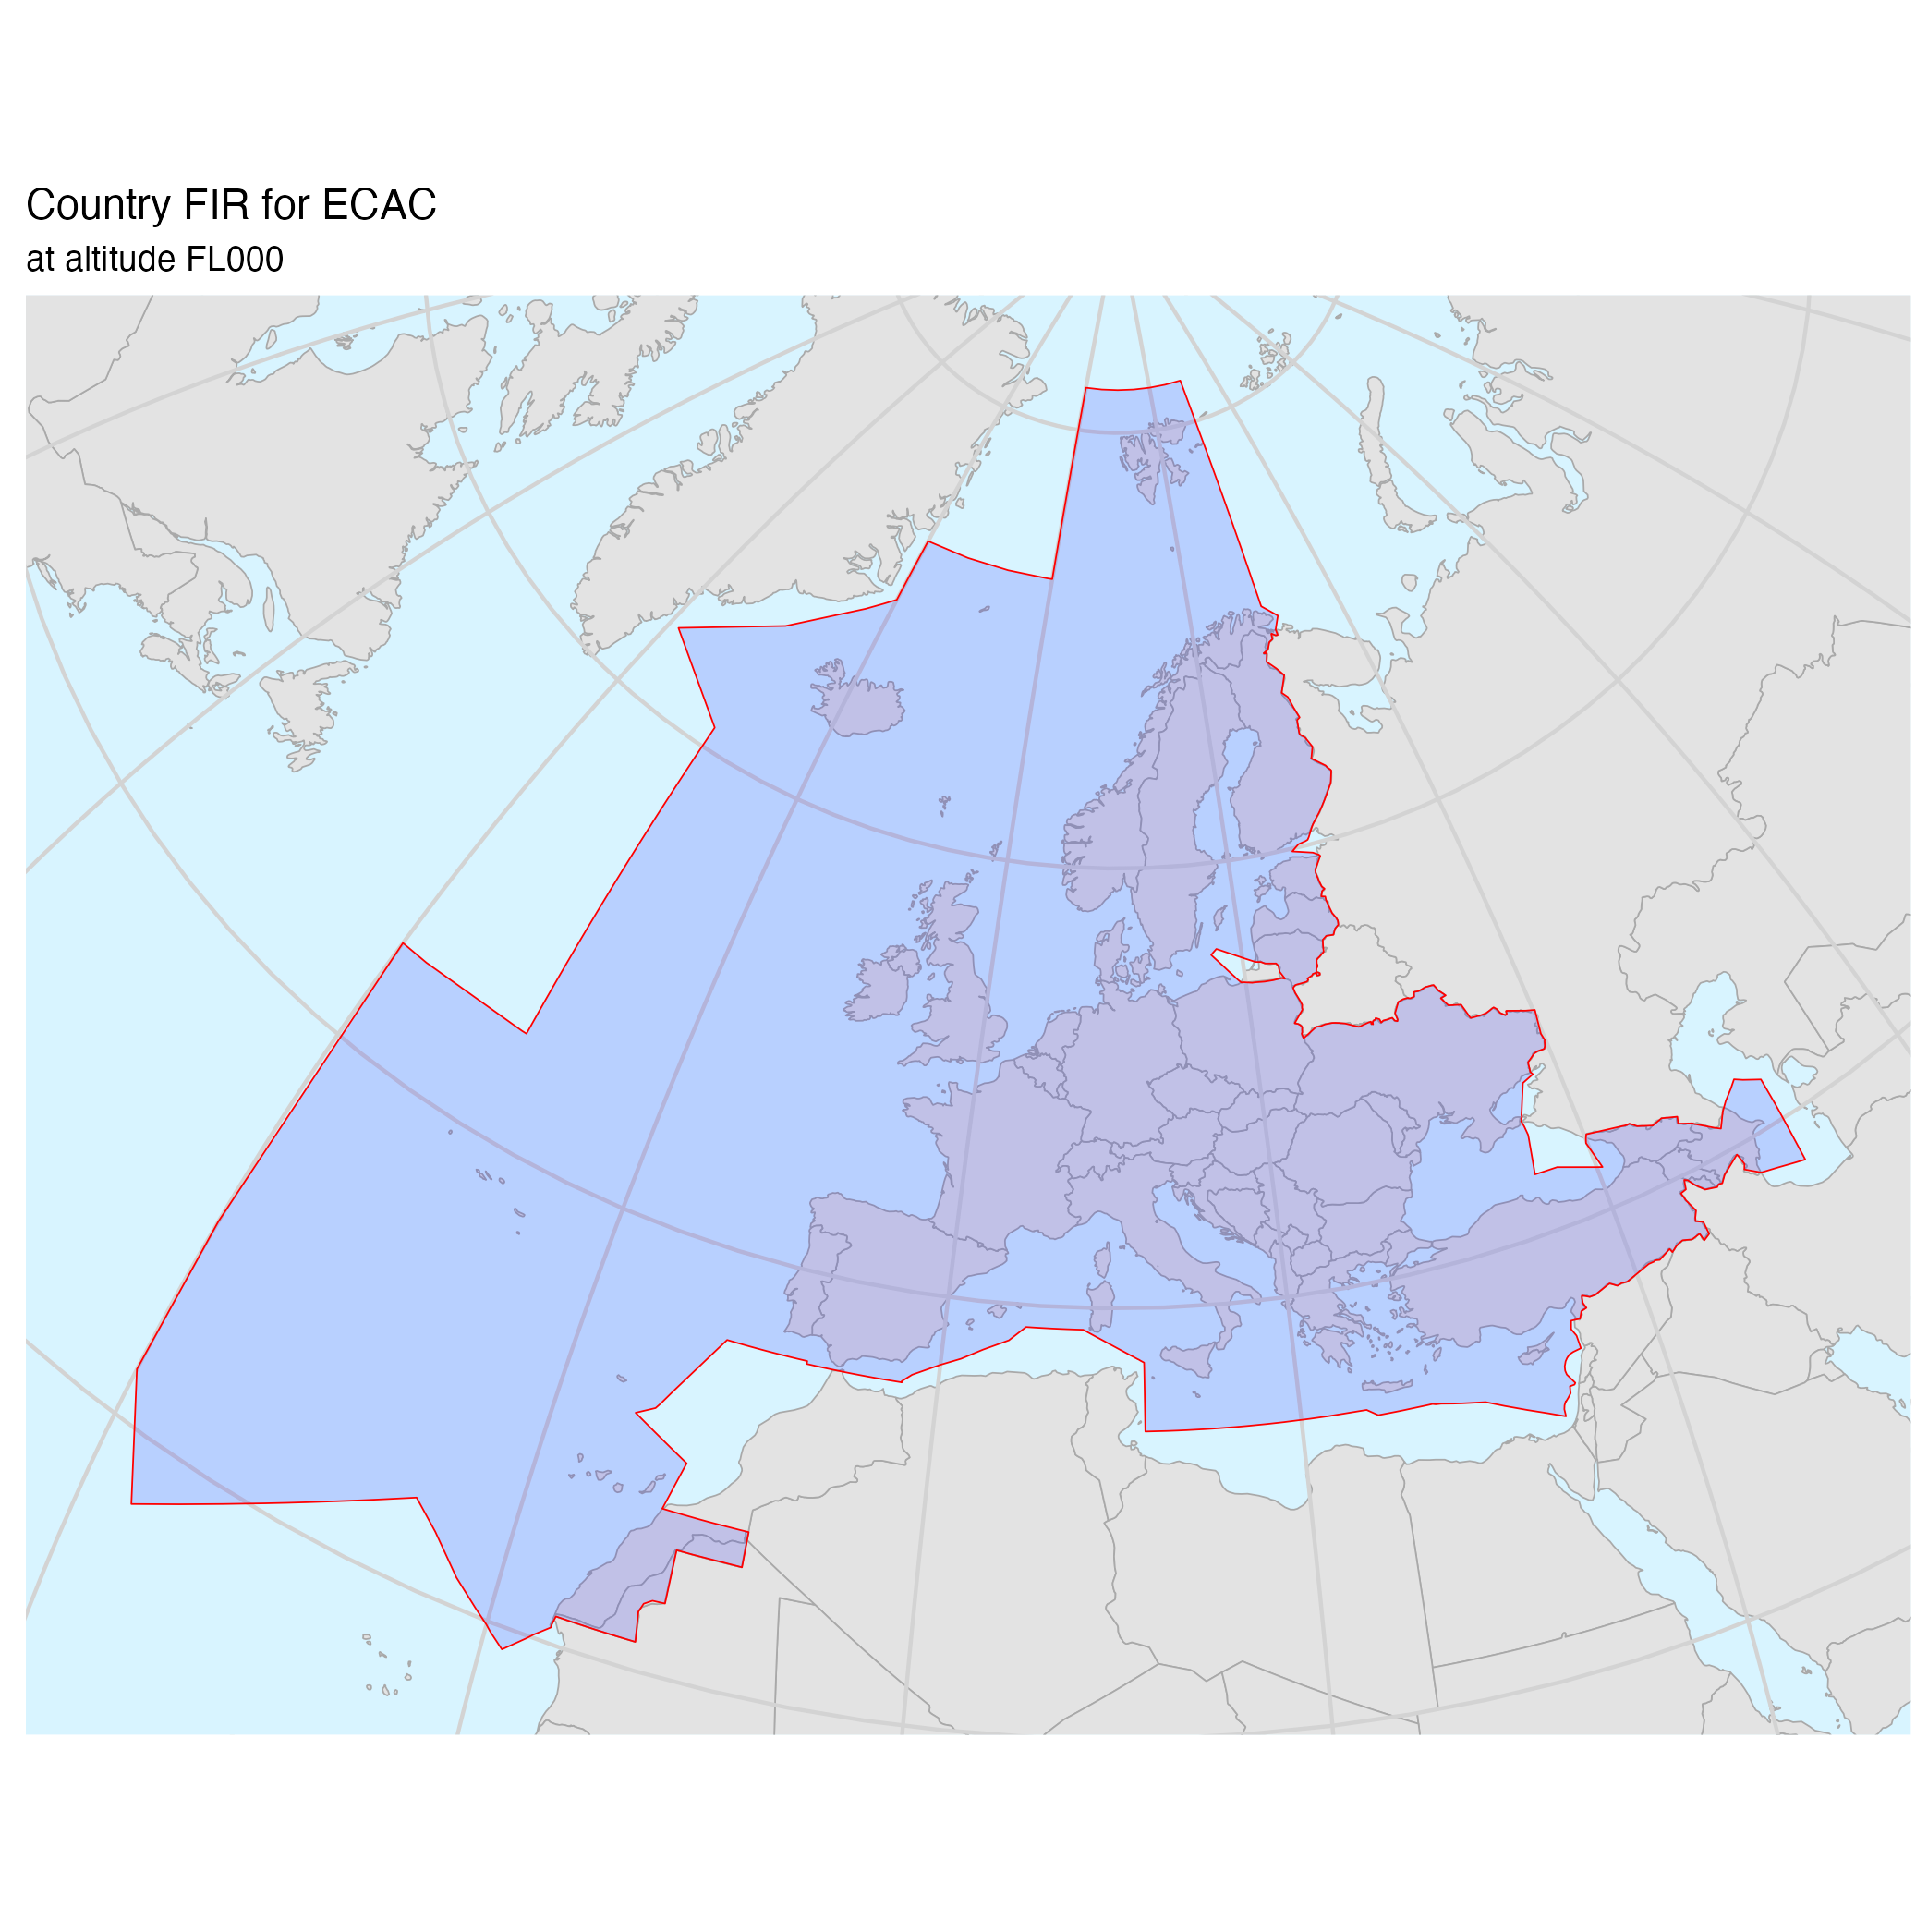
\includegraphics{./figures/ecac_airspace_fir.png}

}

\caption{\label{fig-ecac-airspace-fir}Airspace controlled by ECAC Member
States}

\end{figure}

\part{Traffic and capacity}

\hypertarget{sec-air-traffic-statistics-and-forecasts}{%
\chapter{Air traffic statistics and
forecasts}\label{sec-air-traffic-statistics-and-forecasts}}

\hypertarget{eurocontrol-recommended-value}{%
\section{EUROCONTROL recommended
value}\label{eurocontrol-recommended-value}}

The Statistics and Forecasts (STATFOR) service produces flights and
service units forecasts of future network traffic with a view to help
planners understand and manage risks, identify bottlenecks and
anticipate the needs of airspace users.

\hypertarget{medium-term-forecasts-7-year-timespan}{%
\subsection{Medium-term forecasts (7-year
timespan)}\label{medium-term-forecasts-7-year-timespan}}

The 7-year forecasts give a comprehensive picture of anticipated air
traffic development in Europe for the next seven years. They combine
flight statistics with economic growth and models of other industry
drivers, including costs, airport capacity, passenger numbers, load
factors and aircraft size. Using high and low growth scenarios, they
present a likely range for growth, to help planners manage risks. They
are published biannually, in spring and autumn, covering flights, en
route and terminal service units.

\begin{figure}

{\centering 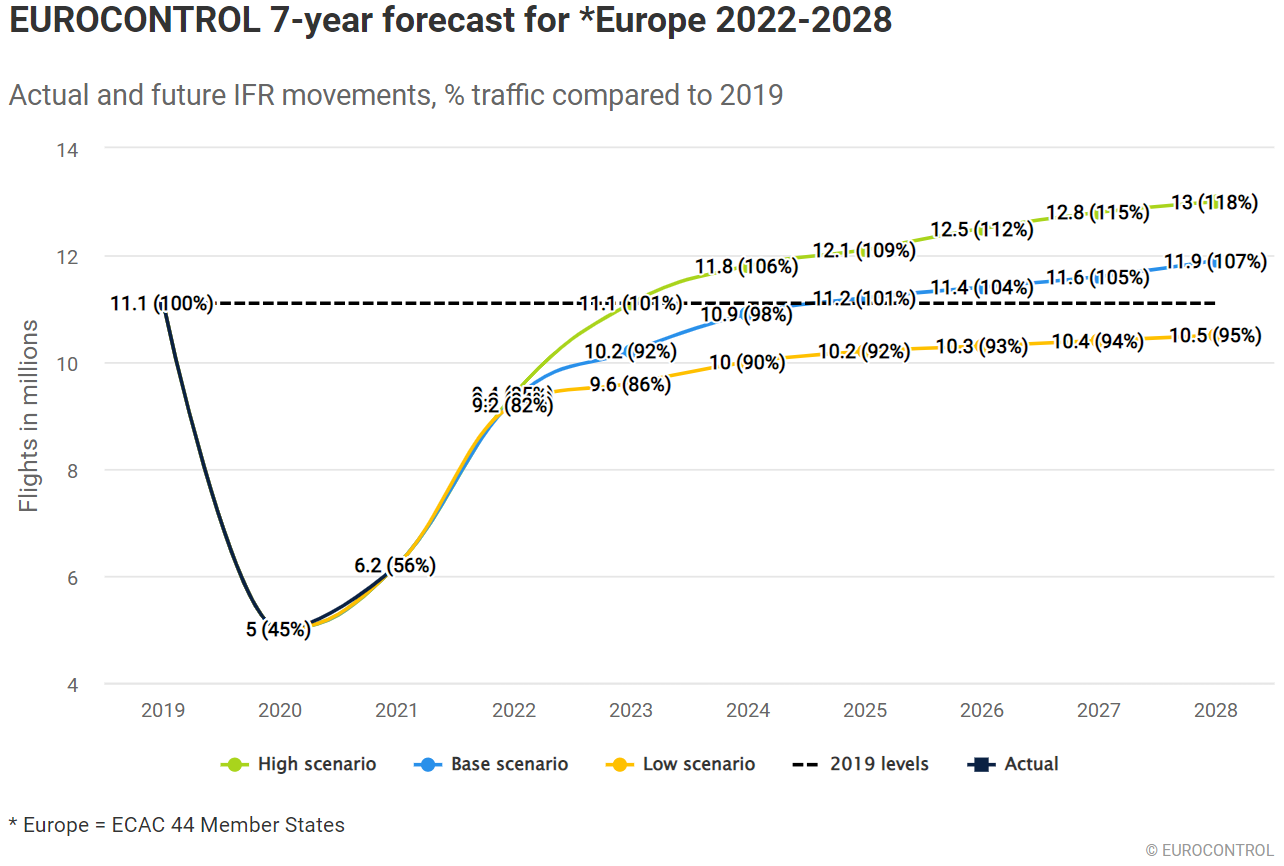
\includegraphics{./figures/forecast_2022-2028.png}

}

\caption{\label{fig-forecast-2022-2028-plot}EUROCONTROL 7-year forecast
2022-2028 (October 2022 release)
\protect\hyperlink{ref-statfor:7year_forecast:2022-2028}{{[}4{]}}}

\end{figure}

The above graph shows the traffic forecast taking account of the impact
of the COVID-19 pandemic. In the base scenario, IFR flights are expected
to get back to 2019 levels by 2025.

Traffic statistics and forecasts can be obtained directly from the
STATFOR Interactive Dashboard
(SID)\protect\hyperlink{ref-ectrl:statfor:sid}{{[}5{]}}.

\hypertarget{long-term-forecasts-20-to-30-year-timespan}{%
\subsection{Long-term forecasts (20 to 30-year
timespan)}\label{long-term-forecasts-20-to-30-year-timespan}}

Twenty/thirty-year forecasts: These forecasts look at a range of
distinct possible scenarios for how the air traffic industry might look
in 20-30 years' time. This allows a range of \emph{what if?} questions
to be explored, for factors inside the industry (e.g.~the growth of
small business jets, or of point-to-point traffic) or outside the
industry (e.g.~the price of oil or environmental constraints).
Twenty/thirty-year forecasts are usually published every two to three
years. In April 2022, EUROCONTROL published its first EUROCONTROL
Aviation Outlook (EAO) looking out to 2050, much further than previous
forecasts. This forecast estimates a future number of flights and CO2
emissions per scenario, in line with aviation's objective of achieving
net-zero CO2 emissions by that date.

\begin{figure}

{\centering 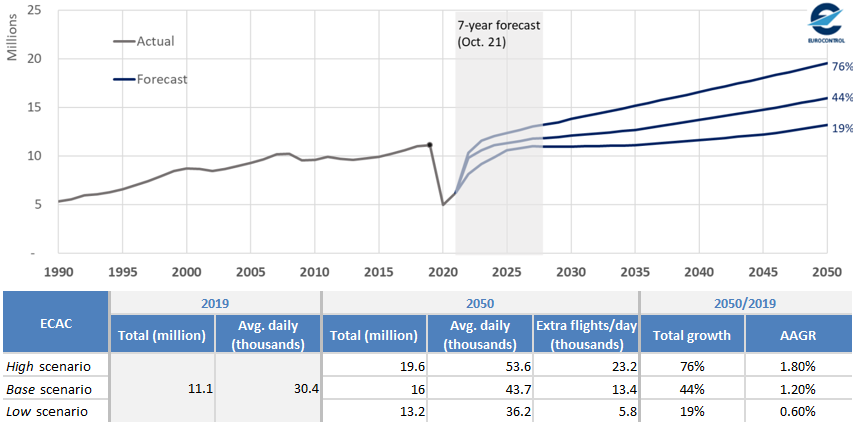
\includegraphics{./figures/eao_2050_flights_base_scenario.png}

}

\caption{\label{fig-Forecast-2050-plot}Flight forecast for Europe, with
total growth between 2019 and 2050}

\end{figure}

In the most-likely Base scenario, the forecast is for 16 million flights
in Europe in 2050, 44\% more than in 2019 -- average growth of 1.2\% per
year.

\begin{figure}

{\centering 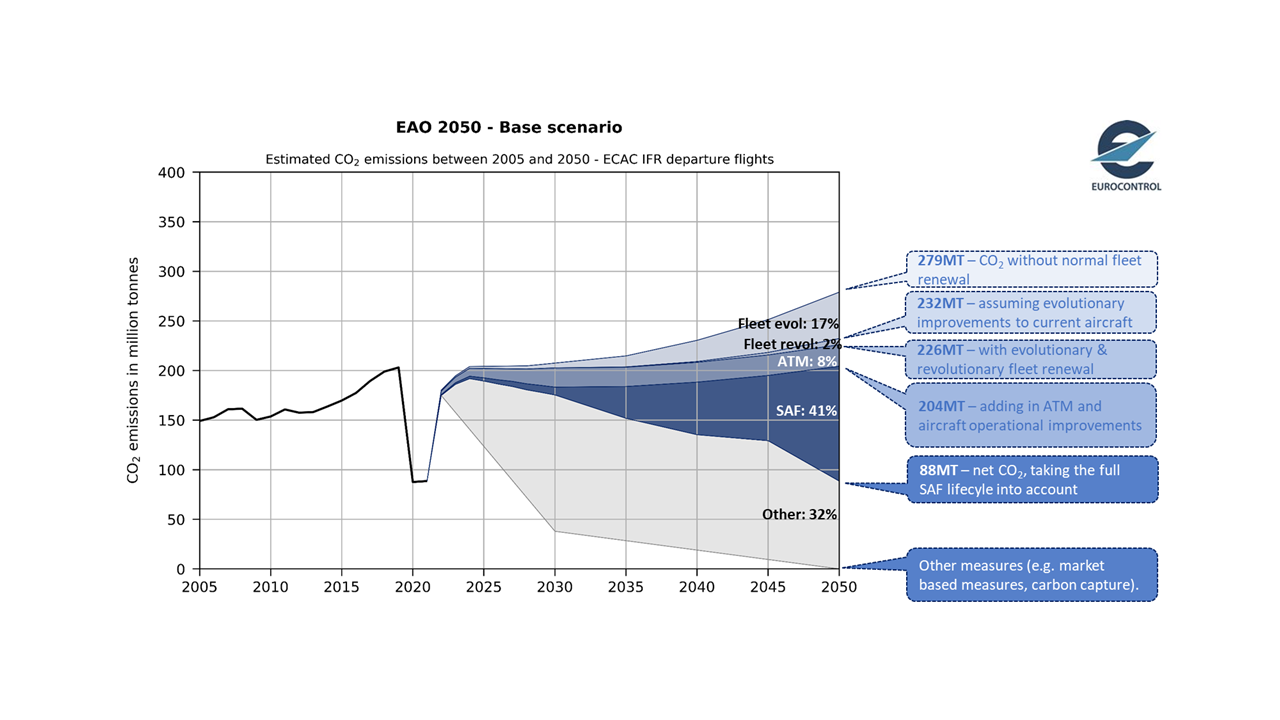
\includegraphics{./figures/eao_2050_base_scenario.png}

}

\caption{\label{fig-co2-emissions-plot}Estimated CO2 emissions between
2005 and 2050 \protect\hyperlink{ref-aviation:outlook2022}{{[}6{]}}}

\end{figure}

The graph in Figure~\ref{fig-co2-emissions-plot} estimates that by 2050,
CO2 emissions, net of SAF, fleet and operational improvements, are
reduced by about 41\% compared to 2005 in the Base scenario.

\hypertarget{service-units-forecasts}{%
\subsection{Service units forecasts}\label{service-units-forecasts}}

Service Units are billed to airlines for the provision of air-traffic
services. They are of two types:

\begin{itemize}
\item
  En-route service units (TSU) that are taxed for the provision of
  en-route air traffic control and are a function of the weight and the
  distance flown within each state over which the concerned aircraft
  flies.
\item
  Terminal Navigation Service Units (TNSU) are taxed for the provision
  of ground services to the airlines for each departure at a given
  airport. They are a function of the weight of the considered aircraft.
\end{itemize}

EUROCONTROL produces a 7-year forecast of Service Units that builds on
the 7-year IFR movements forecast, to which forecasts of the aircraft
weights and distances are added. This Service Units forecast is provided
as a service to states that are part of the Central Route Charges Office
(CRCO) to help them set-up their en-route units rates, if needed. The
Forecast of Service Units in general serves also as a benchmark for the
European Commission to assess the financial aspects of the performance
plans of the states that are bound by the performance and Charging
Scheme according to EU regulations (EU) N°390/201, N°391/2013.

\begin{figure}

{\centering 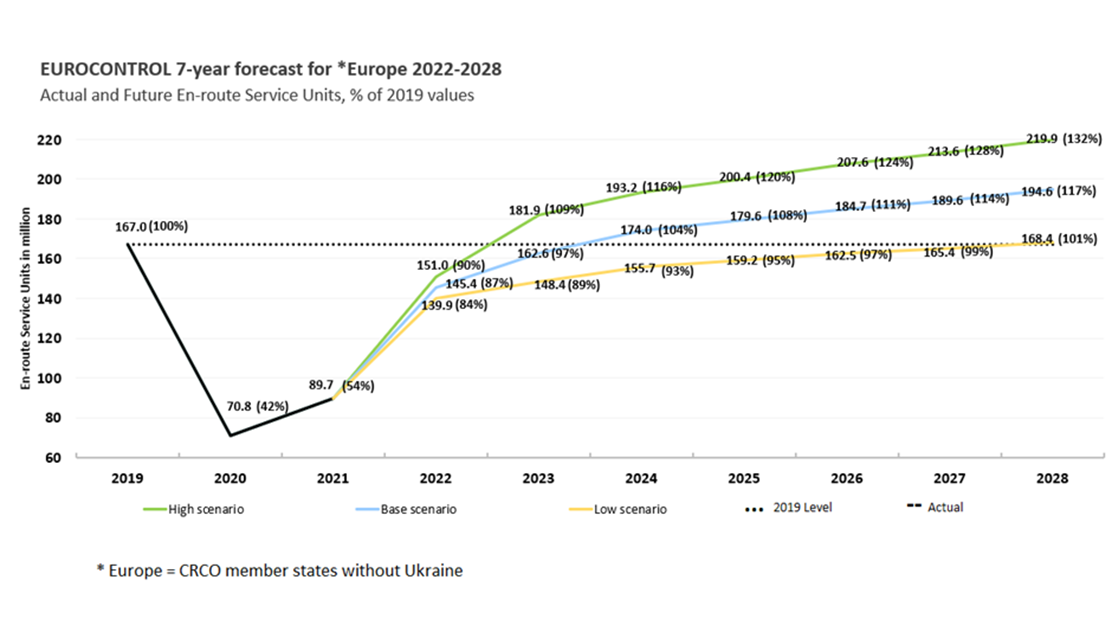
\includegraphics{./figures/forecast_service_units.png}

}

\caption{\label{fig-forecast-service-units-plot}En-route Service Units
7-year Forecast 2022-2028
\protect\hyperlink{ref-statfor:7year_forecast:2022-2028}{{[}4{]}}}

\end{figure}

The above graph (status: October 2022) shows the en-route service units
forecast taking account of the impact of the COVID-19 pandemic.

\hypertarget{when-to-use-the-inputs}{%
\section{When to use the inputs?}\label{when-to-use-the-inputs}}

The objective of STATFOR is to provide statistics and forecasts on IFR
flight movements and service units in Europe (ECAC) and to monitor and
analyse the evolution of the air transport industry.

\hypertarget{related-inputs}{%
\section{Related inputs}\label{related-inputs}}

\begin{itemize}
\tightlist
\item
  Chapter~\ref{sec-medium-term-capacity-planning}
  \protect\hyperlink{sec-medium-term-capacity-planning}{Medium-term
  capacity planning}
\item
  Chapter~\ref{sec-air-traffic-delay}
  \protect\hyperlink{sec-air-traffic-delay}{Air traffic delay}
\item
  Chapter~\ref{sec-cost-of-delay}
  \protect\hyperlink{sec-cost-of-delay}{Cost of delay}
\end{itemize}

\hypertarget{references-1}{%
\section{References}\label{references-1}}

\hypertarget{sec-medium-term-capacity-planning}{%
\chapter{Medium-term capacity
planning}\label{sec-medium-term-capacity-planning}}

\hypertarget{eurocontrol-recommended-sources}{%
\section{EUROCONTROL recommended
sources}\label{eurocontrol-recommended-sources}}

In this document, capacity planning represents the systematic
determination of resource requirements for the projected output over a
specific period of time. It is a dynamic activity that relies on
constantly changing data on the ATM network use, capacity forecasts,
etc.

Given this, below are presented the sources that are recommended to
consult in order to obtain relevant up to date information on capacity
planning.

\begin{itemize}
\item
  \textbf{\emph{EUROCONTROL European Network Operations Plan 2022-2026
  \protect\hyperlink{ref-ectrl:nop:2022}{{[}7{]}}}}

  The European Network Operations Plan (NOP) provides a short- to
  medium-term outlook of the expected ATM network operations and
  performance at network and local level.

  It provides a detailed overview of capacity and flight efficiency
  enhancement measures planned at network level and by each Area Control
  Centre (ACC), a description of the airport performance assessment and
  improvement measures planned at airports generating a high level of
  delay, operational actions planned to be taken by the Network Manager
  and other stakeholders that would respond to the performance targets.
  Furthermore, it provides an assessment of the expected impact from
  these measures on the network.
\item
  \textbf{\emph{EUROCONTROL European Network Operations Plan (NOP) -
  Rolling Seasonal Plann
  \protect\hyperlink{ref-ectrl:nop:rsp}{{[}8{]}}}}

  The European NOP Rolling Seasonal Plan is updated every Friday,
  focusing on the planning of the next six weeks and on the management
  of the execution and implementation of the 5-years NOP. Its aim is to
  facilitate ANSPs and airports planning to match traffic demand in a
  safe, efficient and coordinated manner by providing them with a
  consolidated European network view of the evolution of air traffic.

  More information about network performance (and access to dashboards
  and the archive) can be found at the
  \href{https://www.eurocontrol.int/network-performance}{Network
  Performance page}.
\item
  \textbf{\emph{European ATM Master Plan - implementation plan -- level
  3 \protect\hyperlink{ref-ectrl:mp:ip}{{[}9{]}} and European ATM Master
  Plan -- implementation report -- level 3
  \protect\hyperlink{ref-ectrl:mp:ir}{{[}10{]}}}}

  The
  \href{https://www.eurocontrol.int/portal/european-atm-master-plan-portal}{\textbf{European
  ATM Master Plan}} is the main planning tool for setting ATM
  priorities, ensuring that the SESAR target concept becomes a reality.
  It is an evolving roadmap and the result of collaboration between all
  ATM stakeholders. The Master Plan provides a high-level view of what
  needs to be done in order to deliver a high-performing ATM system,
  while also explaining why and by when. It sets the framework for the
  development activities carried out by the SESAR Joint Undertaking
  (SJU) and deployed by stakeholders in partnership with the SESAR
  Deployment Manager (SDM).

  The \textbf{European ATM Master Plan - implementation plan -- level 3}
  is produced annually and provides the framework for the commonly
  agreed actions to be taken by ECAC stakeholders, in the context of the
  implementation of the SESAR Programme.

  These actions are consolidated in implementation objectives,
  addressing elements in SESAR which have reached the necessary
  operational and technical maturity and for which stakeholders have
  expressed an interest in their operational introduction. They provide
  all civil and military implementing parties (ANSPs, airport operators,
  airspace users and regulators) with a basis for short- to medium-term
  implementation planning.

  The \textbf{European ATM Master Plan - implementation report -- level
  3} maps the evolution of the Master Plan implementation on the four
  phases of the SESAR vision, as defined in the 2020 edition of the
  Executive view of the Master Plan, for the delivery of a Digital
  European Sky.

  The Implementation Objectives constitute the backbone of the Level 3
  and provide all civil and military implementing parties with a basis
  for short- to medium-term implementation planning. It also serves as a
  reference for States/National Supervisory Authorities (NSAs) to fulfil
  their roles regarding the supervision of safe and efficient provision
  of air navigation services as well as the timely implementation of
  SESAR.
\item
  \textbf{\emph{Local Single Sky ImPlementatiom (LSSIP) documents}}
  \protect\hyperlink{ref-ectrl:lssip}{{[}11{]}}

  The Local Single Sky ImPlementation (LSSIP) documents give a
  comprehensive overview of all ATM information for each of the ECAC
  Member States. They also show the ATM capacity forecasts and planning
  targets from NOP. The documents reflect progress made and detail the
  plans for each State for the next five to seven years.

  LSSIP documents, one for each State, are derived from the European
  Single Sky Implementation (ESSIP) (also known as Master Plan Level 3)
  objectives, and stakeholder lines of action cascade down into the
  States.
\end{itemize}

\hypertarget{related-inputs-1}{%
\section{Related inputs}\label{related-inputs-1}}

\begin{itemize}
\item
  Chapter~\ref{sec-air-traffic-statistics-and-forecasts}
  \protect\hyperlink{sec-air-traffic-statistics-and-forecasts}{Air
  traffic statistics and forecasts}
\item
  Chapter~\ref{sec-air-traffic-delay}
  \protect\hyperlink{sec-air-traffic-delay}{Air traffic delay}
\end{itemize}

\hypertarget{references-2}{%
\section{References}\label{references-2}}

\hypertarget{sec-number-of-ifr-flights}{%
\chapter{Number of IFR flights}\label{sec-number-of-ifr-flights}}

\hypertarget{eurocontrol-recommended-values}{%
\section{EUROCONTROL recommended
values}\label{eurocontrol-recommended-values}}

This section presents the evolution of flight movements in Europe (ECAC
area) by flight flow, market segment and aircraft type.

\hypertarget{evolution-of-flights-per-flow-in-2021-compared-to-2019}{%
\subsection{Evolution of flights per flow in 2021 compared to
2019}\label{evolution-of-flights-per-flow-in-2021-compared-to-2019}}

\hypertarget{tbl-ifr-flights-month}{}
\setlength{\LTpost}{0mm}
\begin{longtable}{llllllrc}
\caption{\label{tbl-ifr-flights-month}Evolution of IFR flights in Europe (ECAC) 2019 vs 2021 }\tabularnewline

\toprule
 & \multicolumn{4}{c}{DAIO} & \multicolumn{2}{c}{Total} &  \\ 
\cmidrule(lr){2-5} \cmidrule(lr){6-7}
Month & Departure & Arrival & Internal & Overflight & 2021 & 2019 & 2021 traffic as \% of 2019 \\ 
\midrule
January & $34,972$ & $35,151$ & $206,217$ & $8,984$ & $285,324$ & $787,503$ & $36\%$ \\ 
February & $30,885$ & $30,871$ & $180,689$ & $7,469$ & $249,914$ & $737,763$ & $34\%$ \\ 
March & $37,184$ & $37,174$ & $223,117$ & $9,606$ & $307,081$ & $846,442$ & $36\%$ \\ 
April & $37,685$ & $37,729$ & $241,842$ & $10,136$ & $327,392$ & $906,539$ & $36\%$ \\ 
May & $38,615$ & $38,847$ & $291,508$ & $11,444$ & $380,414$ & $985,862$ & $39\%$ \\ 
June & $45,275$ & $45,437$ & $415,450$ & $12,667$ & $518,829$ & $1,038,128$ & $50\%$ \\ 
July & $62,163$ & $62,118$ & $574,282$ & $13,735$ & $712,298$ & $1,092,562$ & $65\%$ \\ 
August & $64,666$ & $64,778$ & $619,233$ & $14,469$ & $763,146$ & $1,080,554$ & $71\%$ \\ 
September & $61,857$ & $61,777$ & $591,118$ & $13,570$ & $728,322$ & $1,034,322$ & $70\%$ \\ 
October & $64,303$ & $64,142$ & $575,242$ & $15,193$ & $718,880$ & $980,049$ & $73\%$ \\ 
November & $59,573$ & $59,498$ & $483,850$ & $15,986$ & $618,907$ & $801,961$ & $77\%$ \\ 
December & $59,797$ & $59,552$ & $485,033$ & $15,863$ & $620,245$ & $793,617$ & $78\%$ \\ 
Total & $596,975$ & $597,074$ & $4,887,581$ & $149,122$ & $6,230,752$ & $11,085,302$ & $56\%$ \\ 
\bottomrule
\end{longtable}
\begin{minipage}{\linewidth}
\emph{Source: \href{https://www.eurocontrol.int/dashboard/statfor-interactive-dashboard}{STATFOR Interactive Dashboard}}\\
\end{minipage}

Please note that the comparison between 2021 and 2019 in
Table~\ref{tbl-ifr-flights-month} is due to the fact that 2019 is the
last year where the traffic levels were not affected by the COVID-19
pandemic, allowing for a more realistic comparison of the flight levels.

\hypertarget{flights-by-market-segment-in-europe-ecac-in-2021-compared-to-2019}{%
\subsection{Flights by market segment in Europe (ECAC) in 2021 compared
to
2019}\label{flights-by-market-segment-in-europe-ecac-in-2021-compared-to-2019}}

\hypertarget{tbl-flights-per-market-segment}{}
\setlength{\LTpost}{0mm}
\begin{longtable}{llclclc}
\caption{\label{tbl-flights-per-market-segment}Flights by market segment in Europe (ECAC) 2019-2021 }\tabularnewline

\toprule
Market segment & 2019 & Share of Total 2019 & 2020 & Share of Total 2020 & 2021 & Share of Total 2021 \\ 
\midrule
Mainline & $3,991,685$ & $36\%$ & $1,479,557$ & $30\%$ & $1,816,909$ & $29\%$ \\ 
Lowcost & $3,493,913$ & $32\%$ & $1,243,422$ & $25\%$ & $1,610,239$ & $26\%$ \\ 
Regional Aircraft & $1,643,854$ & $15\%$ & $746,765$ & $15\%$ & $861,587$ & $14\%$ \\ 
Business Aviation & $683,473$ & $6\%$ & $513,628$ & $10\%$ & $709,398$ & $11\%$ \\ 
All-Cargo & $368,362$ & $3\%$ & $389,914$ & $8\%$ & $419,824$ & $7\%$ \\ 
Other Types & $372,796$ & $3\%$ & $309,283$ & $6\%$ & $363,712$ & $6\%$ \\ 
Charter & $382,218$ & $3\%$ & $162,798$ & $3\%$ & $303,384$ & $5\%$ \\ 
Military & $149,001$ & $1\%$ & $133,711$ & $3\%$ & $145,699$ & $2\%$ \\ 
Total & $11,085,302$ & $100\%$ & $4,979,078$ & $100\%$ & $6,230,752$ & $100\%$ \\ 
\bottomrule
\end{longtable}
\begin{minipage}{\linewidth}
\emph{Source: \href{https://www.eurocontrol.int/dashboard/statfor-interactive-dashboard}{STATFOR Interactive Dashboard}}\\
\end{minipage}

EUROCONTROL market segments were updated in 2022 and saw the
``Traditional Scheduled'' segment split into ``Mainline'' and
``Regional'' according to EUROCONTROL Market Segment Rules
\protect\hyperlink{ref-ectl:market:seg:2022}{{[}12{]}}.

In 2021 the total number of flights went up 25.1\% compared to 2020, but
was at 56.2\% of 2019 flight levels (pre-COVID-19). Compared with 2019,
only two segments increased in 2021 and they were All-Cargo (+13.9\%)
and Business Aviation (+3.8\%). The Mainline (-54.5\%), Low-Cost
(-53.9\%) and Regional (-47.6\%) segments were the most affected, along
with the Charter segment which went down by -20.6\% in 2021 (vs 2019).

\hypertarget{top-20-number-of-flights-by-civil-aviation-aircraft-in-europe-ecac-in-2021}{%
\subsection{Top 20 number of flights by civil aviation aircraft in
Europe (ECAC) in
2021}\label{top-20-number-of-flights-by-civil-aviation-aircraft-in-europe-ecac-in-2021}}

\hypertarget{tbl-flights-per-aircraft-type}{}
\setlength{\LTpost}{0mm}
\begin{longtable}{llcc}
\caption{\label{tbl-flights-per-aircraft-type}Top 20 flights by aircraft type in Europe (ECAC) in 2021 }\tabularnewline

\toprule
Aircraft Type & Flights & Proportion & Cumulative \\ 
\midrule
B738 & $1,098,879$ & $19\%$ & $19\%$ \\ 
A320 & $760,204$ & $13\%$ & $32\%$ \\ 
A319 & $312,864$ & $5\%$ & $38\%$ \\ 
A20N & $310,527$ & $5\%$ & $43\%$ \\ 
A321 & $193,590$ & $3\%$ & $47\%$ \\ 
A21N & $150,955$ & $3\%$ & $49\%$ \\ 
B77W & $132,040$ & $2\%$ & $51\%$ \\ 
E190 & $131,891$ & $2\%$ & $54\%$ \\ 
AT76 & $109,491$ & $2\%$ & $56\%$ \\ 
B789 & $98,893$ & $2\%$ & $57\%$ \\ 
AT75 & $85,711$ & $1\%$ & $59\%$ \\ 
A333 & $82,982$ & $1\%$ & $60\%$ \\ 
DH8D & $81,496$ & $1\%$ & $62\%$ \\ 
E195 & $76,625$ & $1\%$ & $63\%$ \\ 
B734 & $76,322$ & $1\%$ & $64\%$ \\ 
B77L & $65,577$ & $1\%$ & $66\%$ \\ 
B38M & $63,990$ & $1\%$ & $67\%$ \\ 
CRJ9 & $63,696$ & $1\%$ & $68\%$ \\ 
B737 & $62,673$ & $1\%$ & $69\%$ \\ 
DH8A & $62,082$ & $1\%$ & $70\%$ \\ 
Other types & $1,730,263$ & $30\%$ & $100\%$ \\ 
Total & $5,750,751$ & $100\%$ & NA \\ 
\bottomrule
\end{longtable}
\begin{minipage}{\linewidth}
\emph{Source: \href{https://www.eurocontrol.int/forecasting}{EUROCONTROL STATFOR}}\\
\end{minipage}

In 2021 there were 301 different civil aircraft types operating IFR
flights in Europe. About 70\% of the flights were carried out by the 20
aircraft types listed in Table~\ref{tbl-flights-per-aircraft-type}.
Please note that the values presented in
Table~\ref{tbl-flights-per-aircraft-type} focuses on the civil aviation
flights (i.e.~excluding the military and other categories), resulting in
a difference in the total flights as compared with
Table~\ref{tbl-flights-per-market-segment} and
Table~\ref{tbl-ifr-flights-month}.

\hypertarget{daily-average-of-ifr-flights-2016-to-2021}{%
\subsection{Daily average of IFR flights, 2016 to
2021}\label{daily-average-of-ifr-flights-2016-to-2021}}

Figure~\ref{fig-average-daily-ifr-flights-plot} shows the daily average
number of IFR flights \textbf{EU-wide} between 2016 and 2021.

\begin{figure}

{\centering 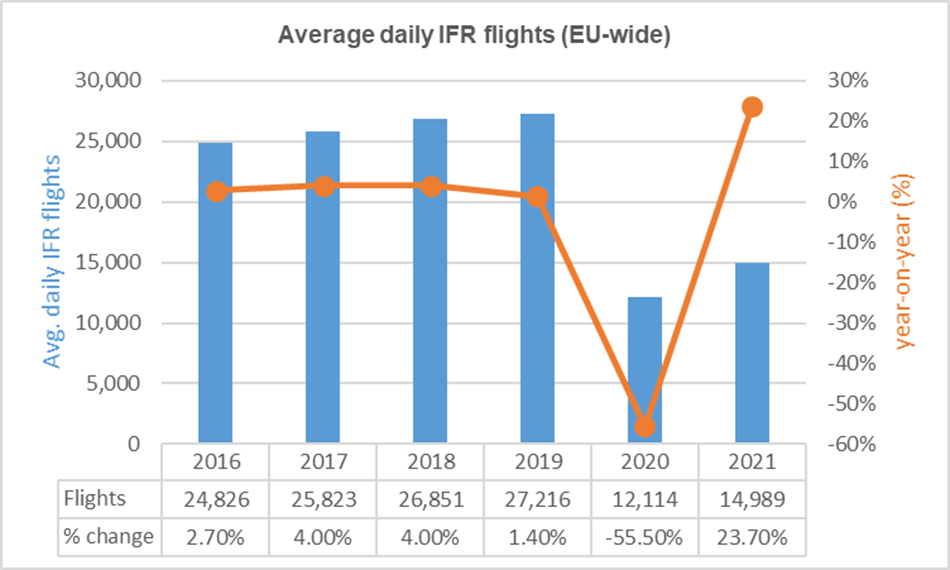
\includegraphics{./figures/average_daily_flights.png}

}

\caption{\label{fig-average-daily-ifr-flights-plot}Daily average numbers
of IFR flights \protect\hyperlink{ref-prb:dashboard:2022}{{[}13{]}}}

\end{figure}

\hypertarget{when-to-use-the-input}{%
\section{When to use the input?}\label{when-to-use-the-input}}

This input is recommended to be used in situations where an overview of
the historical evolution in the number of flights is required, namely
grouped according to different criteria.

\hypertarget{related-inputs-2}{%
\section{Related inputs}\label{related-inputs-2}}

\begin{itemize}
\tightlist
\item
  Chapter~\ref{sec-ifr-flight-information-per-market-segment}
  \protect\hyperlink{sec-ifr-flight-information-per-market-segment}{IFR
  flight information per operator segment}
\item
  Chapter~\ref{sec-fleet-age} \protect\hyperlink{sec-fleet-age}{Fleet
  age}
\item
  Chapter~\ref{sec-fleet-size} \protect\hyperlink{sec-fleet-size}{Fleet
  size}
\item
  Chapter~\ref{sec-fleet-cns-capability}
  \protect\hyperlink{sec-fleet-cns-capability}{Fleet CNS capability}
\end{itemize}

\hypertarget{references-3}{%
\section{References}\label{references-3}}

\hypertarget{sec-air-traffic-delay}{%
\chapter{Air traffic delay}\label{sec-air-traffic-delay}}

\hypertarget{eurocontrol-recommended-values-1}{%
\section{EUROCONTROL recommended
values}\label{eurocontrol-recommended-values-1}}

The sections below present the evolution in reported delays taking two
perspectives:

\begin{enumerate}
\def\labelenumi{\arabic{enumi}.}
\item
  The view of airlines and passengers considering all causes of delay
\item
  A zoom-in to the view of the Network Manager focusing on Air Traffic
  Flow Management (ATFM) delays
\end{enumerate}

\hypertarget{all-causes-of-delay}{%
\subsection{All causes of delay}\label{all-causes-of-delay}}

Figure~\ref{fig-all-causes-delay} presents an \textbf{overview of all
causes of delay reported by the airlines} in 2020 and 2021. The figures
presented are estimated by the EUROCONTROL
\href{https://www.eurocontrol.int/network-performance}{Central Office of
Delay Analysis (CODA)}, and are calculated based on the comparison of
the scheduled and actual flight timings
\protect\hyperlink{ref-coda2021}{{[}14{]}}. They can be used in studies
that look into the different causes of flight delay experienced by
passengers and airlines.

\begin{figure}

{\centering 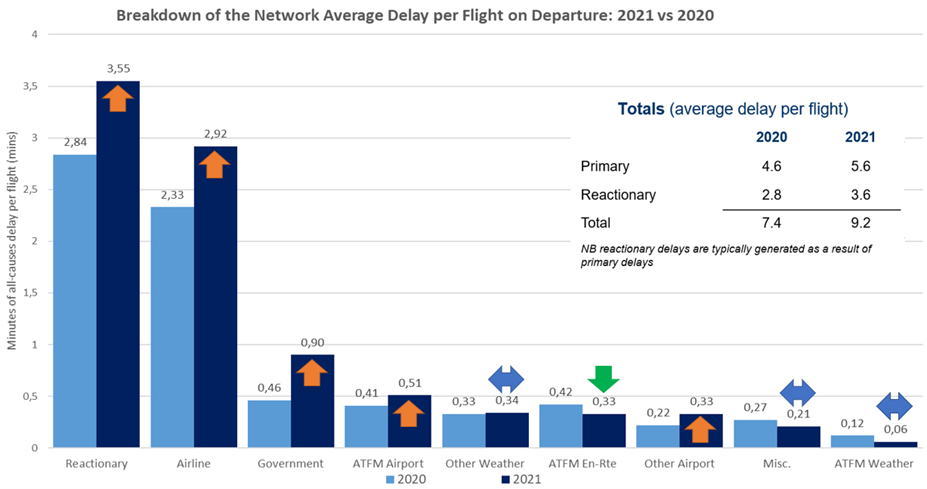
\includegraphics{./figures/delay_causes.png}

}

\caption{\label{fig-all-causes-delay}Breakdown of the network average
delay per flight on departure: 2021 vs 2020
\protect\hyperlink{ref-coda2021}{{[}14{]}}}

\end{figure}

The ATFM delay constitutes only a fraction of primary delay from all
causes, and around half of all delay is reactionary (i.e., delay caused
by late arrival of aircraft, crew, passengers or baggage from previous
journeys) rather than primary (i.e., delay other than reactionary).

\hypertarget{atfm-delay}{%
\subsection{ATFM delay}\label{atfm-delay}}

Looking specifically into \textbf{ATFM delay},
Figure~\ref{fig-atfm-delay} shows the daily traffic and traffic flow
delay per flight (en-route and at airport) for the period 2012-2021. The
figures presented are calculated by the Network Manager based on the
flight plans and include the planned ATFM delays due to the restrictions
that may be applied in the airspace
\protect\hyperlink{ref-nm2022}{{[}15{]}}.

\begin{figure}

{\centering \includegraphics{./figures/atfm_delay.png}

}

\caption{\label{fig-atfm-delay}Average daily traffic and ATFM delay per
flight 2012-2022 \protect\hyperlink{ref-nm2022}{{[}15{]}}}

\end{figure}

\hypertarget{when-to-use-the-input-1}{%
\section{When to use the input?}\label{when-to-use-the-input-1}}

We recommend using all causes of delay provided by CODA when analysing
the impacts on airlines or on passengers/society (e.g., an airline
upgrading the avionics in their aircraft; airport expansion, etc.). On
the other hand, ATFM delay is recommended to be used when analysing
projects aiming at improving flow management.

Furthermore, since primary delay shows the delay that is due to direct
triggers, it is recommended to be used when analysing updates that would
impact the non-reactionary delays.

\hypertarget{comment}{%
\section{Comment}\label{comment}}

Looking at both figures above, it can be observed that the ATFM delay,
both at the airport and en-route, is higher when looking at the numbers
provided by the airlines rather than that observed by the Network
Manager. This occurs because the delay numbers provided by the Network
Manager account for the so-called planned delay due to restrictions in
the airspace, while the numbers provided by the airlines cover the total
delay they attribute to ATFM, whether they come from the restrictions or
any other planned ATFM delays

Another important point to take into consideration when analysing the
recommended values is the impact of COVID-19 pandemic. Both, the
all-causes delay and the ATFM delay were impacted by the significant
reduction in air traffic in 2020 and 2021, resulting in a strong drop in
the total delay duration. Thus, when looking into these numbers it is
equally important to consider the situation prior to 2020. For the
All-causes delay this information can be found in the previous editions
of CODA Digest, available in EUROCONTROL library
\protect\hyperlink{ref-ectllibrary}{{[}16{]}}.

\hypertarget{related-inputs-3}{%
\section{Related inputs}\label{related-inputs-3}}

\begin{itemize}
\tightlist
\item
  Chapter~\ref{sec-air-traffic-statistics-and-forecasts}
  \protect\hyperlink{sec-air-traffic-statistics-and-forecasts}{Air
  traffic statistics and forecast}
\item
  Chapter~\ref{sec-cost-of-delay}
  \protect\hyperlink{sec-cost-of-delay}{Cost of delay}
\end{itemize}

\hypertarget{references-4}{%
\section{References}\label{references-4}}

\hypertarget{sec-transit-time}{%
\chapter{Transit time}\label{sec-transit-time}}

\hypertarget{eurocontrol-recommended-values-2}{%
\section{EUROCONTROL Recommended
Values}\label{eurocontrol-recommended-values-2}}

The transit time in an ANSP represents the \textbf{average time flown by
aircraft controlled in this airspace over a year}.
Table~\ref{tbl-transit-time} provides an overview of the average transit
time (expressed in minutes) per ANSP in 2019.

The data that was used to build this table can be accessed on
\href{https://ansperformance.eu/data/}{AIU portal}. You can find there
data for more recent years.

\hypertarget{tbl-transit-time}{}
\setlength{\LTpost}{0mm}
\begin{longtable}{llc}
\caption{\label{tbl-transit-time}Average transit time per country }\tabularnewline

\toprule
ANSP & State & Transit time (minutes) \\ 
\midrule
Albcontrol & Albania & 13 \\ 
ANS CR & Czech Republic & 20 \\ 
ANS Finland & Finland & 28 \\ 
ARMATS & Armenia & 16 \\ 
Austro Control & Austria & 19 \\ 
AVINOR (Continental) & Norway & 37 \\ 
BULATSA & Bulgaria & 20 \\ 
Croatia Control & Croatia & 22 \\ 
DCAC Cyprus & Cyprus & 29 \\ 
DFS & Germany & 30 \\ 
DHMI & Türkiye & 59 \\ 
DSNA & France & 45 \\ 
EANS & Estonia & 20 \\ 
ENAIRE & Spain & 46 \\ 
ENAV & Italy & 39 \\ 
HCAA & Greece & 42 \\ 
HungaroControl & Hungary & 17 \\ 
IAA & Ireland & 30 \\ 
LFV & Sweden & 35 \\ 
LGS & Latvia & 18 \\ 
LPS & Slovakia & 12 \\ 
LVNL & Netherlands & 17 \\ 
MATS & Malta & 41 \\ 
M-NAV & North Macedonia & 10 \\ 
MOLDATSA & Republic of Moldova & 14 \\ 
MUAC & NA & 22 \\ 
NATS (Continental) & United Kingdom & 37 \\ 
NAV Portugal (Continental) & Portugal & 40 \\ 
NAVIAIR & Denmark & 20 \\ 
Oro Navigacija & Lithuania & 16 \\ 
PANSA & Poland & 34 \\ 
ROMATSA & Romania & 32 \\ 
SAKAERONAVIGATSIA & Georgia & 22 \\ 
skeyes & Belgium & 11 \\ 
Skyguide & Switzerland & 17 \\ 
Slovenia Control & Slovenia & 11 \\ 
SMATSA & Serbia \& Montenegro & 23 \\ 
UkSATSE & Ukraine & 39 \\ 
\bottomrule
\end{longtable}
\begin{minipage}{\linewidth}
\emph{Source: \href{https://ansperformance.eu/data/}{EUROCONTROL Aviation Intelligence Unit}}\\
\end{minipage}

\hypertarget{description}{%
\section{Description}\label{description}}

This metric is the ratio between the total flight hours controlled and
the IFR flights controlled, where:

\begin{itemize}
\item
  Total IFR flight-hours controlled is the sum of the flight-hours
  controlled over the year by the ANSP. For a given flight the
  flight-hours controlled are computed using information available in
  the Network Manager database as the difference between the exit time
  and the entry time in the controlled airspace
\item
  IFR movements controlled is the number of flights that have been
  controlled over the year by the ANSP
\end{itemize}

In \textbf{?@fig-transit-time}, the range of transit time values for the
vast majority of ANSPs in Europe can be observed (Note: the scope is
limited to the 38 ANSPs reporting to the
\href{https://ansperformance.eu/about/prc/}{Performance Review
Commission}). The European average in terms of flight time is 31 minutes
per ANSP. A difference of 49 minutes between the highest (DHMI Türkiye)
and the lowest (M-NAV North Macedonia) transit time can also be observed
-- this represents a ratio of almost 6 or a Standard Deviation of around
12.

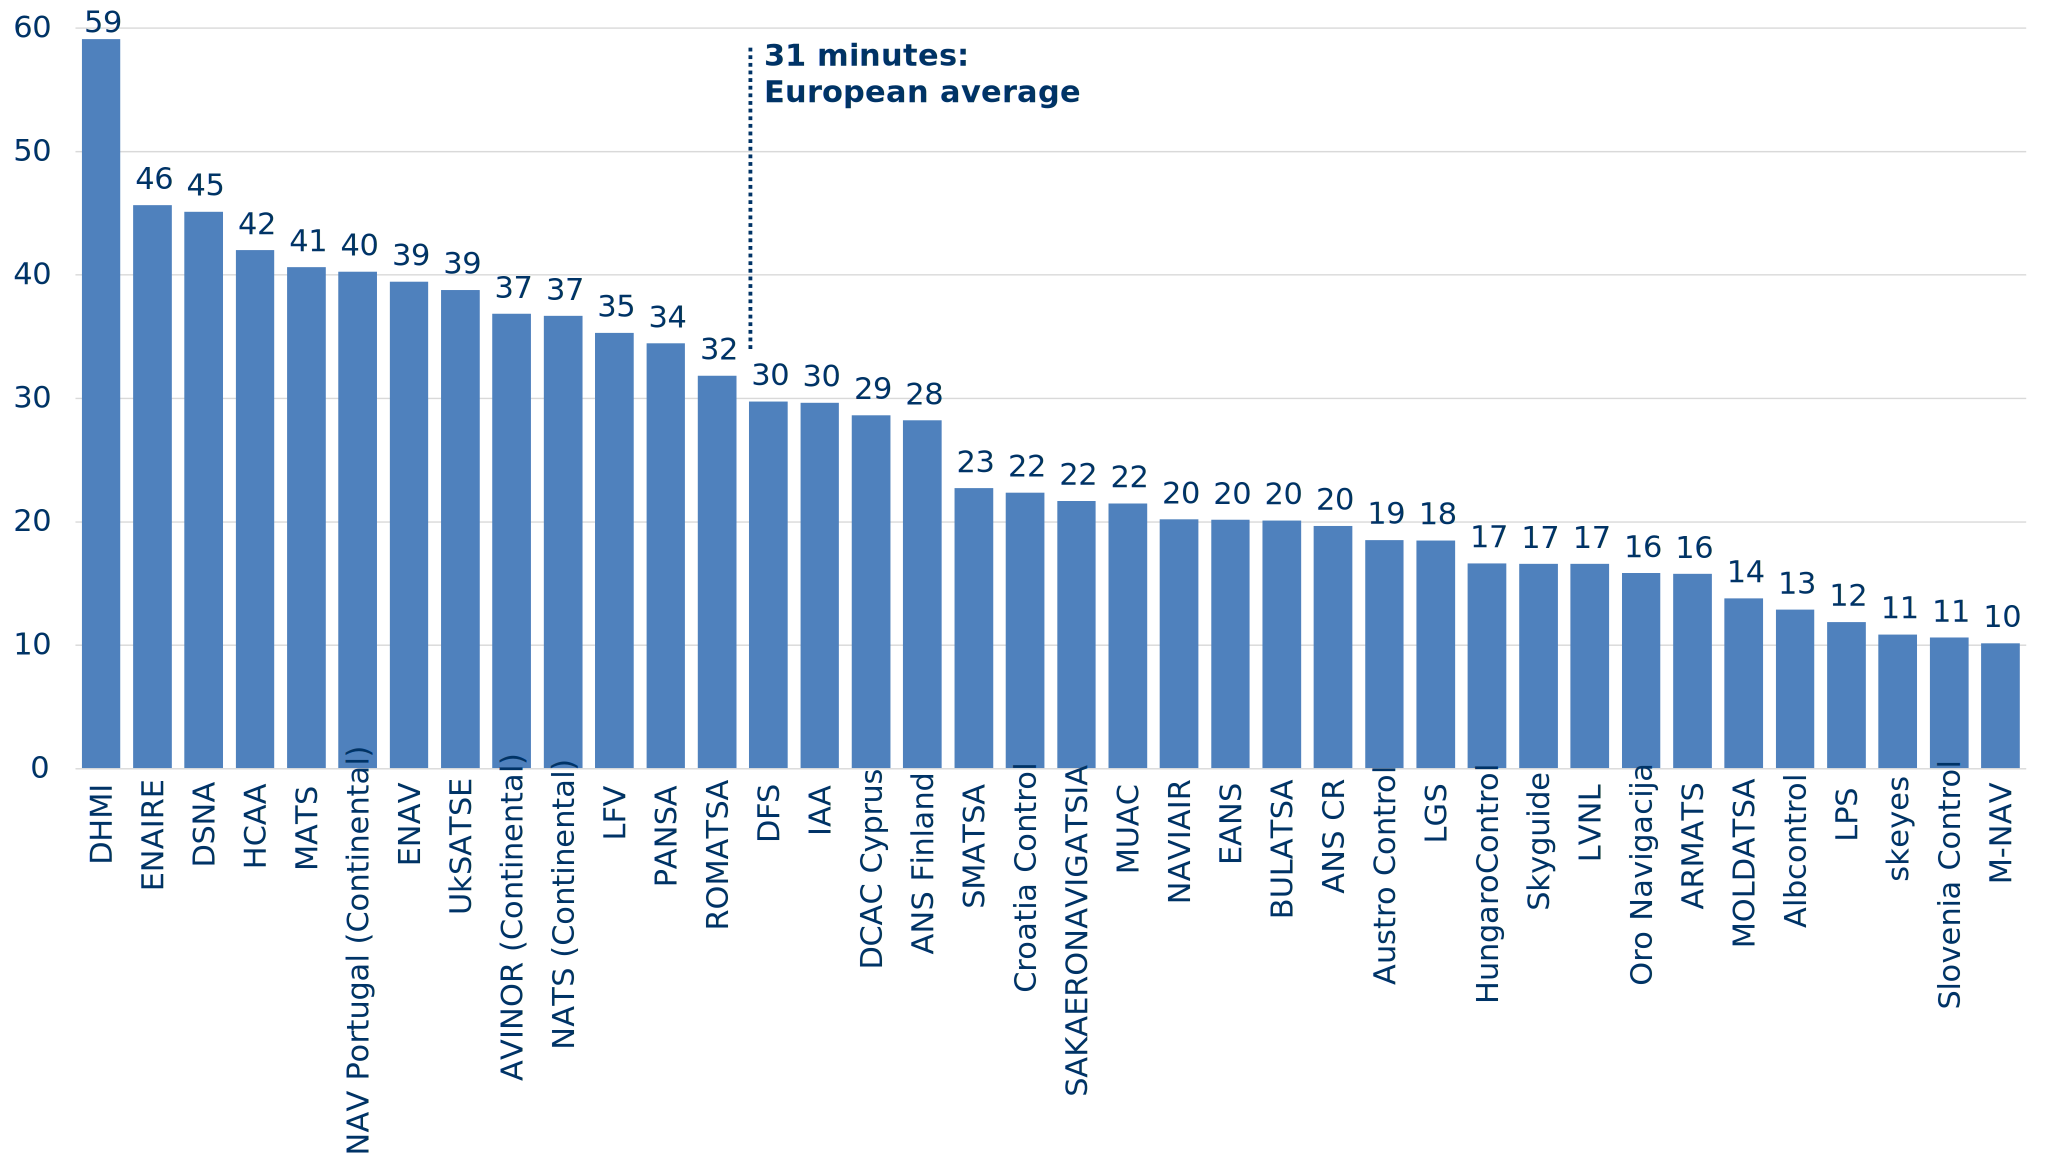
\includegraphics{./figures/transit_time.svg} \emph{Source: EUROCONTROL}

\hypertarget{when-to-use-the-input-2}{%
\section{When to use the input?}\label{when-to-use-the-input-2}}

This input is recommended for those projects where the flying time in a
giver country or a set of countries is key to the assessment. As an
example, it has previously been used for several CNS related studies, in
particular when studying the cost of communication services that depend
on connection times.

\hypertarget{comments}{%
\section{Comments}\label{comments}}

The data was recorded by the Network Manager (NM) for the 38 ANSPs that
were part of the ACE Report in 2019
\protect\hyperlink{ref-ace2019}{{[}17{]}}. For a few ANSPs, the data
reported show slight differences with the NM records, as ANSPs tend to
communicate their own traffic data. The differences are explained by the
different counting methodology in IFR airport movements for training
flights.

\hypertarget{related-inputs-4}{%
\section{Related inputs}\label{related-inputs-4}}

\begin{itemize}
\tightlist
\item
  Chapter~\ref{sec-medium-term-capacity-planning}
  \protect\hyperlink{sec-medium-term-capacity-planning}{Medium-term
  capacity planning}
\end{itemize}

\hypertarget{references-5}{%
\section{References}\label{references-5}}

\part{Environment}

\hypertarget{sec-rate-of-fuel-burn}{%
\chapter{Rate of fuel burn}\label{sec-rate-of-fuel-burn}}

This chapter is being updated.

For the latest officially published version, please refer to
\href{https://www.eurocontrol.int/sites/default/files/2021-03/eurocontrol-standard-inputs-economic-analysis-ed-9.pdf}{EUROCONTROL
Standard Inputs for Economic Analyses - Edition 9}

\hypertarget{sec-amount-of-emissions-released-by-fuel-burn}{%
\chapter{Amount of emissions released by fuel
burn}\label{sec-amount-of-emissions-released-by-fuel-burn}}

\hypertarget{eurocontrol-recommended-values-3}{%
\section{EUROCONTROL recommended
values}\label{eurocontrol-recommended-values-3}}

This input represents the amount of emissions produced by combustion of
aviation fuel, focusing on the main types of pollutants.

\hypertarget{tbl-emissions-per-kg-fuel}{}
\begin{longtable}{lc}
\caption{\label{tbl-emissions-per-kg-fuel}Emissions per kg of fuel burnt }\tabularnewline

\toprule
Pollutant & Amount of emissions (kg) \\ 
\midrule
CO2 & 3.15000 \\ 
H2O & 1.23700 \\ 
SO2 & 0.00084 \\ 
\bottomrule
\end{longtable}

\emph{Source:
\href{https://www.eurocontrol.int/publication/european-aviation-fuel-burn-and-emissions-inventory-system-feis-european-environment}{EUROCONTROL
(2018). European Aviation Fuel Burn and Emissions Inventory System for
the European Environment Agency}}

\hypertarget{when-to-use-the-input-3}{%
\section{When to use the input?}\label{when-to-use-the-input-3}}

This input is recommended for a wide use in assessments that focus on
the assessment of environmental impact from the burning of fuel at any
stage of the flight.

\hypertarget{comments-1}{%
\section{Comments}\label{comments-1}}

The Committee on Aviation Environmental Protection (CAEP), a technical
committee of the ICAO Council, recommends the use a conversion factor of
\textbf{3.16 g of CO2 per gram of Jet A.} The 3.16 value can be found in
ICAO Doc 9889, 1st edition, 2011, and other documents.

However, in Europe, as early as 2009, Commission Decision 2009/339/EC
indicated an \textbf{emission factor of 3.15 for the mass conversion
from Jet A to CO\textsubscript{2}} for the period after January 2021.

In view of the above, emission factor 3.15 should continue to be used in
SESAR 2020, for the sake of internal consistency within the program,
unless the EU ETS decides to move to 3.16.

Factor 3.16 should be used when the evaluation concerns comparisons with
studies carried out within the ICAO framework or using the factor
recommended by ICAO, in order to ensure external consistency.

\hypertarget{related-inputs-5}{%
\section{Related inputs}\label{related-inputs-5}}

\begin{itemize}
\item
  Chapter~\ref{sec-rate-of-fuel-burn}
  \protect\hyperlink{sec-rate-of-fuel-burn}{Rate of fuel burn}
\item
  Chapter~\ref{sec-cost-of-emissions}
  \protect\hyperlink{sec-cost-of-emissions}{Cost of emissions}
\item
  Chapter~\ref{sec-ifr-flight-information-per-market-segment}
  \protect\hyperlink{sec-ifr-flight-information-per-market-segment}{IFR
  flight information per market segment}
\end{itemize}

\hypertarget{references-6}{%
\section{References}\label{references-6}}

{[}\protect\hyperlink{ref-eaer2022}{{[}18{]}}{]}\protect\hyperlink{ref-eea:2019}{{[}19{]}}\protect\hyperlink{ref-easaICAOAircraftEngine}{{[}20{]}}

\hypertarget{sec-cost-of-emissions}{%
\chapter{Cost of emissions}\label{sec-cost-of-emissions}}

\hypertarget{eurocontrol-recommended-values-4}{%
\section{EUROCONTROL recommended
values}\label{eurocontrol-recommended-values-4}}

The data provided in the following sub-sections shows an estimation of
the cost of CO\textsubscript{2} and other aircraft pollutants released
by the combustion of aviation fuel.

\hypertarget{air-pollution}{%
\subsection{Air pollution}\label{air-pollution}}

According to the Handbook on the external costs of transport
\protect\hyperlink{ref-ecdgmove2019}{{[}21{]}}, for air pollution costs,
the marginal costs are virtually equal to the average costs. This is due
to the fact that the dose-response relationships between the emissions
of air pollutants and health effects are nearly linear.

\hypertarget{tbl-marginal-pollution-cost}{}
\setlength{\LTpost}{0mm}
\begin{longtable}{lcclccc}
\caption{\label{tbl-marginal-pollution-cost}Marginal air pollution costs of aviation }\tabularnewline

\toprule
Type of flight & Distance (km) & Emissions class & Example of aircraft type & Cost per LTO & Cost per pax km (€-cent) & Cost per pax \\ 
\midrule
Short-haul & 500 & Low & Bombardier CRJ900 & $\text{EUR}120.00$ & $\text{EUR}0.33$ & $\text{EUR}1.68$ \\ 
NA & 500 & High & Embraer 170 & $\text{EUR}162.00$ & $\text{EUR}0.36$ & $\text{EUR}1.80$ \\ 
Medium-haul & 1500 & Low & Airbus 320 & $\text{EUR}196.00$ & $\text{EUR}0.08$ & $\text{EUR}1.32$ \\ 
NA & 1500 & High & Boeing 737 & $\text{EUR}219.00$ & $\text{EUR}0.13$ & $\text{EUR}1.87$ \\ 
NA & 3000 & Low & Airbus 320 & $\text{EUR}260.00$ & $\text{EUR}0.06$ & $\text{EUR}1.74$ \\ 
NA & 3000 & High & Boeing 737 & $\text{EUR}290.00$ & $\text{EUR}0.08$ & $\text{EUR}2.48$ \\ 
Long-haul & 5000 & Low & Airbus 340 & $\text{EUR}595.00$ & $\text{EUR}0.04$ & $\text{EUR}2.01$ \\ 
NA & 5000 & High & Boeing 777 & $\text{EUR}987.00$ & $\text{EUR}0.05$ & $\text{EUR}2.28$ \\ 
NA & 15000 & Low & Airbus 340 & $\text{EUR}843.00$ & $\text{EUR}0.02$ & $\text{EUR}2.86$ \\ 
NA & 15000 & High & Boeing 777 & $\text{EUR}1,397.00$ & $\text{EUR}0.02$ & $\text{EUR}3.22$ \\ 
\bottomrule
\end{longtable}
\begin{minipage}{\linewidth}
\emph{Source: \href{https://data.europa.eu/doi/10.2832/51388}{European Commission (2019), Handbook on the external costs of transport}}\\
\end{minipage}

\hypertarget{climate-change}{%
\subsection{Climate change}\label{climate-change}}

One of the approaches to monetise the climate change costs is to
estimate the CO\textsubscript{2} cost avoidance, in compliance with the
provisions of Paris Climate Agreement. The table below provides an
estimate of CO2 equivalent cost avoidance for short and medium term. It
shows a low, medium and high estimate of these values. The values were
adjusted to 2022 prices based on inflation.

\hypertarget{tbl-climate-change-cost}{}
\setlength{\LTpost}{0mm}
\begin{longtable}{lccc}
\caption{\label{tbl-climate-change-cost}Climate change avoidance costs in € per tonne of CO2 equivalent }\tabularnewline

\toprule
  & Low & Medium & High \\ 
\midrule
Short and medium run (up to 2030) & $\text{EUR}71.00$ & $\text{EUR}119.00$ & $\text{EUR}224.00$ \\ 
Long run (from 2040 to 2060) & $\text{EUR}185.00$ & $\text{EUR}319.00$ & $\text{EUR}590.00$ \\ 
\bottomrule
\end{longtable}
\begin{minipage}{\linewidth}
\emph{Source: \href{https://data.europa.eu/doi/10.2832/51388}{European Commission (2019), Handbook on the external costs of transport}}\\
\end{minipage}

\hypertarget{other-possible-values}{%
\subsection{Other possible values}\label{other-possible-values}}

The well-to-tank emissions costs represent the costs linked to the
production of all different type of energy sources, which leads to
emissions and other externalities. It includes the extraction of energy,
processing, transport and transmission, building of energy plants, etc.
These emissions are part of the most relevant emissions when it comes to
transportation.

Table~\ref{tbl-wtt-costs} presents the estimated cost of well-to-tank
emissions from aviation based on an analysis of 33 selected EU airports.
They are expressed in 2022 prices, adjusted from 2019 according to the
indexation.

\hypertarget{tbl-wtt-costs}{}
\setlength{\LTpost}{0mm}
\begin{longtable}{lccc}
\caption{\label{tbl-wtt-costs}Total and average well-to-tank costs for aviation for 33 selected EU
airports }\tabularnewline

\toprule
  & Total cost (bn €) & €-cents per pkm & €-cents per pax \\ 
\midrule
Short-haul (< 1,500 km) & $\text{EUR}1.1$ & $\text{EUR}1.2$ & $\text{EUR}6.6$ \\ 
Medium-haul (1,500 km > 5,000 km) & $\text{EUR}2.4$ & $\text{EUR}0.8$ & $\text{EUR}14.4$ \\ 
Long-haul (> 5,000 km) & $\text{EUR}6.6$ & $\text{EUR}1.0$ & $\text{EUR}80.6$ \\ 
\bottomrule
\end{longtable}
\begin{minipage}{\linewidth}
\emph{Source: \href{https://data.europa.eu/doi/10.2832/51388}{European Commission (2019), Handbook on the external costs of transport}}\\
\end{minipage}

\textbf{?@tbl-wtt-pullution-costs} presents the damage cost factors used
for calculation of the emissions impacts. The prices are expressed in €
per kg and were adjusted to 2022 prices from 2016.

\hypertarget{tbl-wtt-pollution-costs}{}
\begin{longtable}{lcccc}
\caption{\label{tbl-wtt-pollution-costs}Well-to-tank air pollution costs. Damage cost estimates for EU27+UK }\tabularnewline

\toprule
  & NOx & NMVOC & SO2 & PM2.5 (exhaust) \\ 
\midrule
EU27+UK & $\text{EUR}12.9$ & $\text{EUR}1.4$ & $\text{EUR}12.9$ & $\text{EUR}23.0$ \\ 
\bottomrule
\end{longtable}

\hypertarget{further-reading}{%
\section{Further reading}\label{further-reading}}

Below are listed some sources that may be interesting to consult in the
frame of this topic:

\begin{itemize}
\item
  \href{https://www.eurocontrol.int/publication/european-aviation-environmental-report-2022}{EUROCONTROL
  (2022), European Environmental Report}
\item
  \href{https://ec.europa.eu/clima/policies/ets/auctioning_en}{European
  Commission Climate Action}
\item
  \href{https://uk-air.defra.gov.uk/library/reports?report_id=1006}{UK
  Department for Environment, Food and Rural Affairs (DEFRA) (2020), Air
  quality damage cost update 2020}
\end{itemize}

\hypertarget{related-inputs-6}{%
\section{Related inputs}\label{related-inputs-6}}

Chapter~\ref{sec-amount-of-emissions-released-by-fuel-burn}
\protect\hyperlink{sec-amount-of-emissions-released-by-fuel-burn}{Amount
of emissions released by fuel burn}

Chapter~\ref{sec-rate-of-fuel-burn}
\protect\hyperlink{ec-rate-of-fuel-burn}{Rate of fuel burn}

\hypertarget{references-7}{%
\section{References}\label{references-7}}

\hypertarget{sec-cost-of-noise}{%
\chapter{Cost of noise}\label{sec-cost-of-noise}}

This chapter is being updated.

For the latest officially published version, please refer to
\href{https://www.eurocontrol.int/sites/default/files/2021-03/eurocontrol-standard-inputs-economic-analysis-ed-9.pdf}{EUROCONTROL
Standard Inputs for Economic Analyses - Edition 9}

\hypertarget{sec-shadow-cost-of-carbon}{%
\chapter{Shadow cost of carbon}\label{sec-shadow-cost-of-carbon}}

\hypertarget{eurocontrol-recommended-values-5}{%
\section{EUROCONTROL recommended
values}\label{eurocontrol-recommended-values-5}}

The shadow cost of carbon is the cost of carbon required to drive the
economy to meet the 1.5°C global temperature target set by the
Intergovernmental Panel on Climate Change (IPCC). The values have been
estimated based on the data provided by the European Investment Bank in
their 2021-2025 roadmap \protect\hyperlink{ref-eib2020}{{[}22{]}} and
represent the cost in euros per tonne of CO2 equivalent.

The input is an adjustment of the EIB recommended values to reflect the
most realistic cost of meeting the
\href{https://unfccc.int/process-and-meetings/the-paris-agreement/the-paris-agreement}{UN
Paris agreement} to limit global warming well below 2 degrees Celsius,
ideally 1.5 -- compared to pre-industrial levels
\protect\hyperlink{ref-ipcc2018}{{[}23{]}}. Please note this input does
not refer to the traditional \emph{market price} but to the \emph{shadow
cost of carbon}, i.e.~considering externalities and future policies. The
original EIB proposed inputs are expressed in 2016 prices
\protect\hyperlink{ref-eib2020}{{[}22{]}} and have been adjusted to 2021
price levels using the values provided in
Table~\ref{tbl-inflation-table}.

\begin{figure}

{\centering 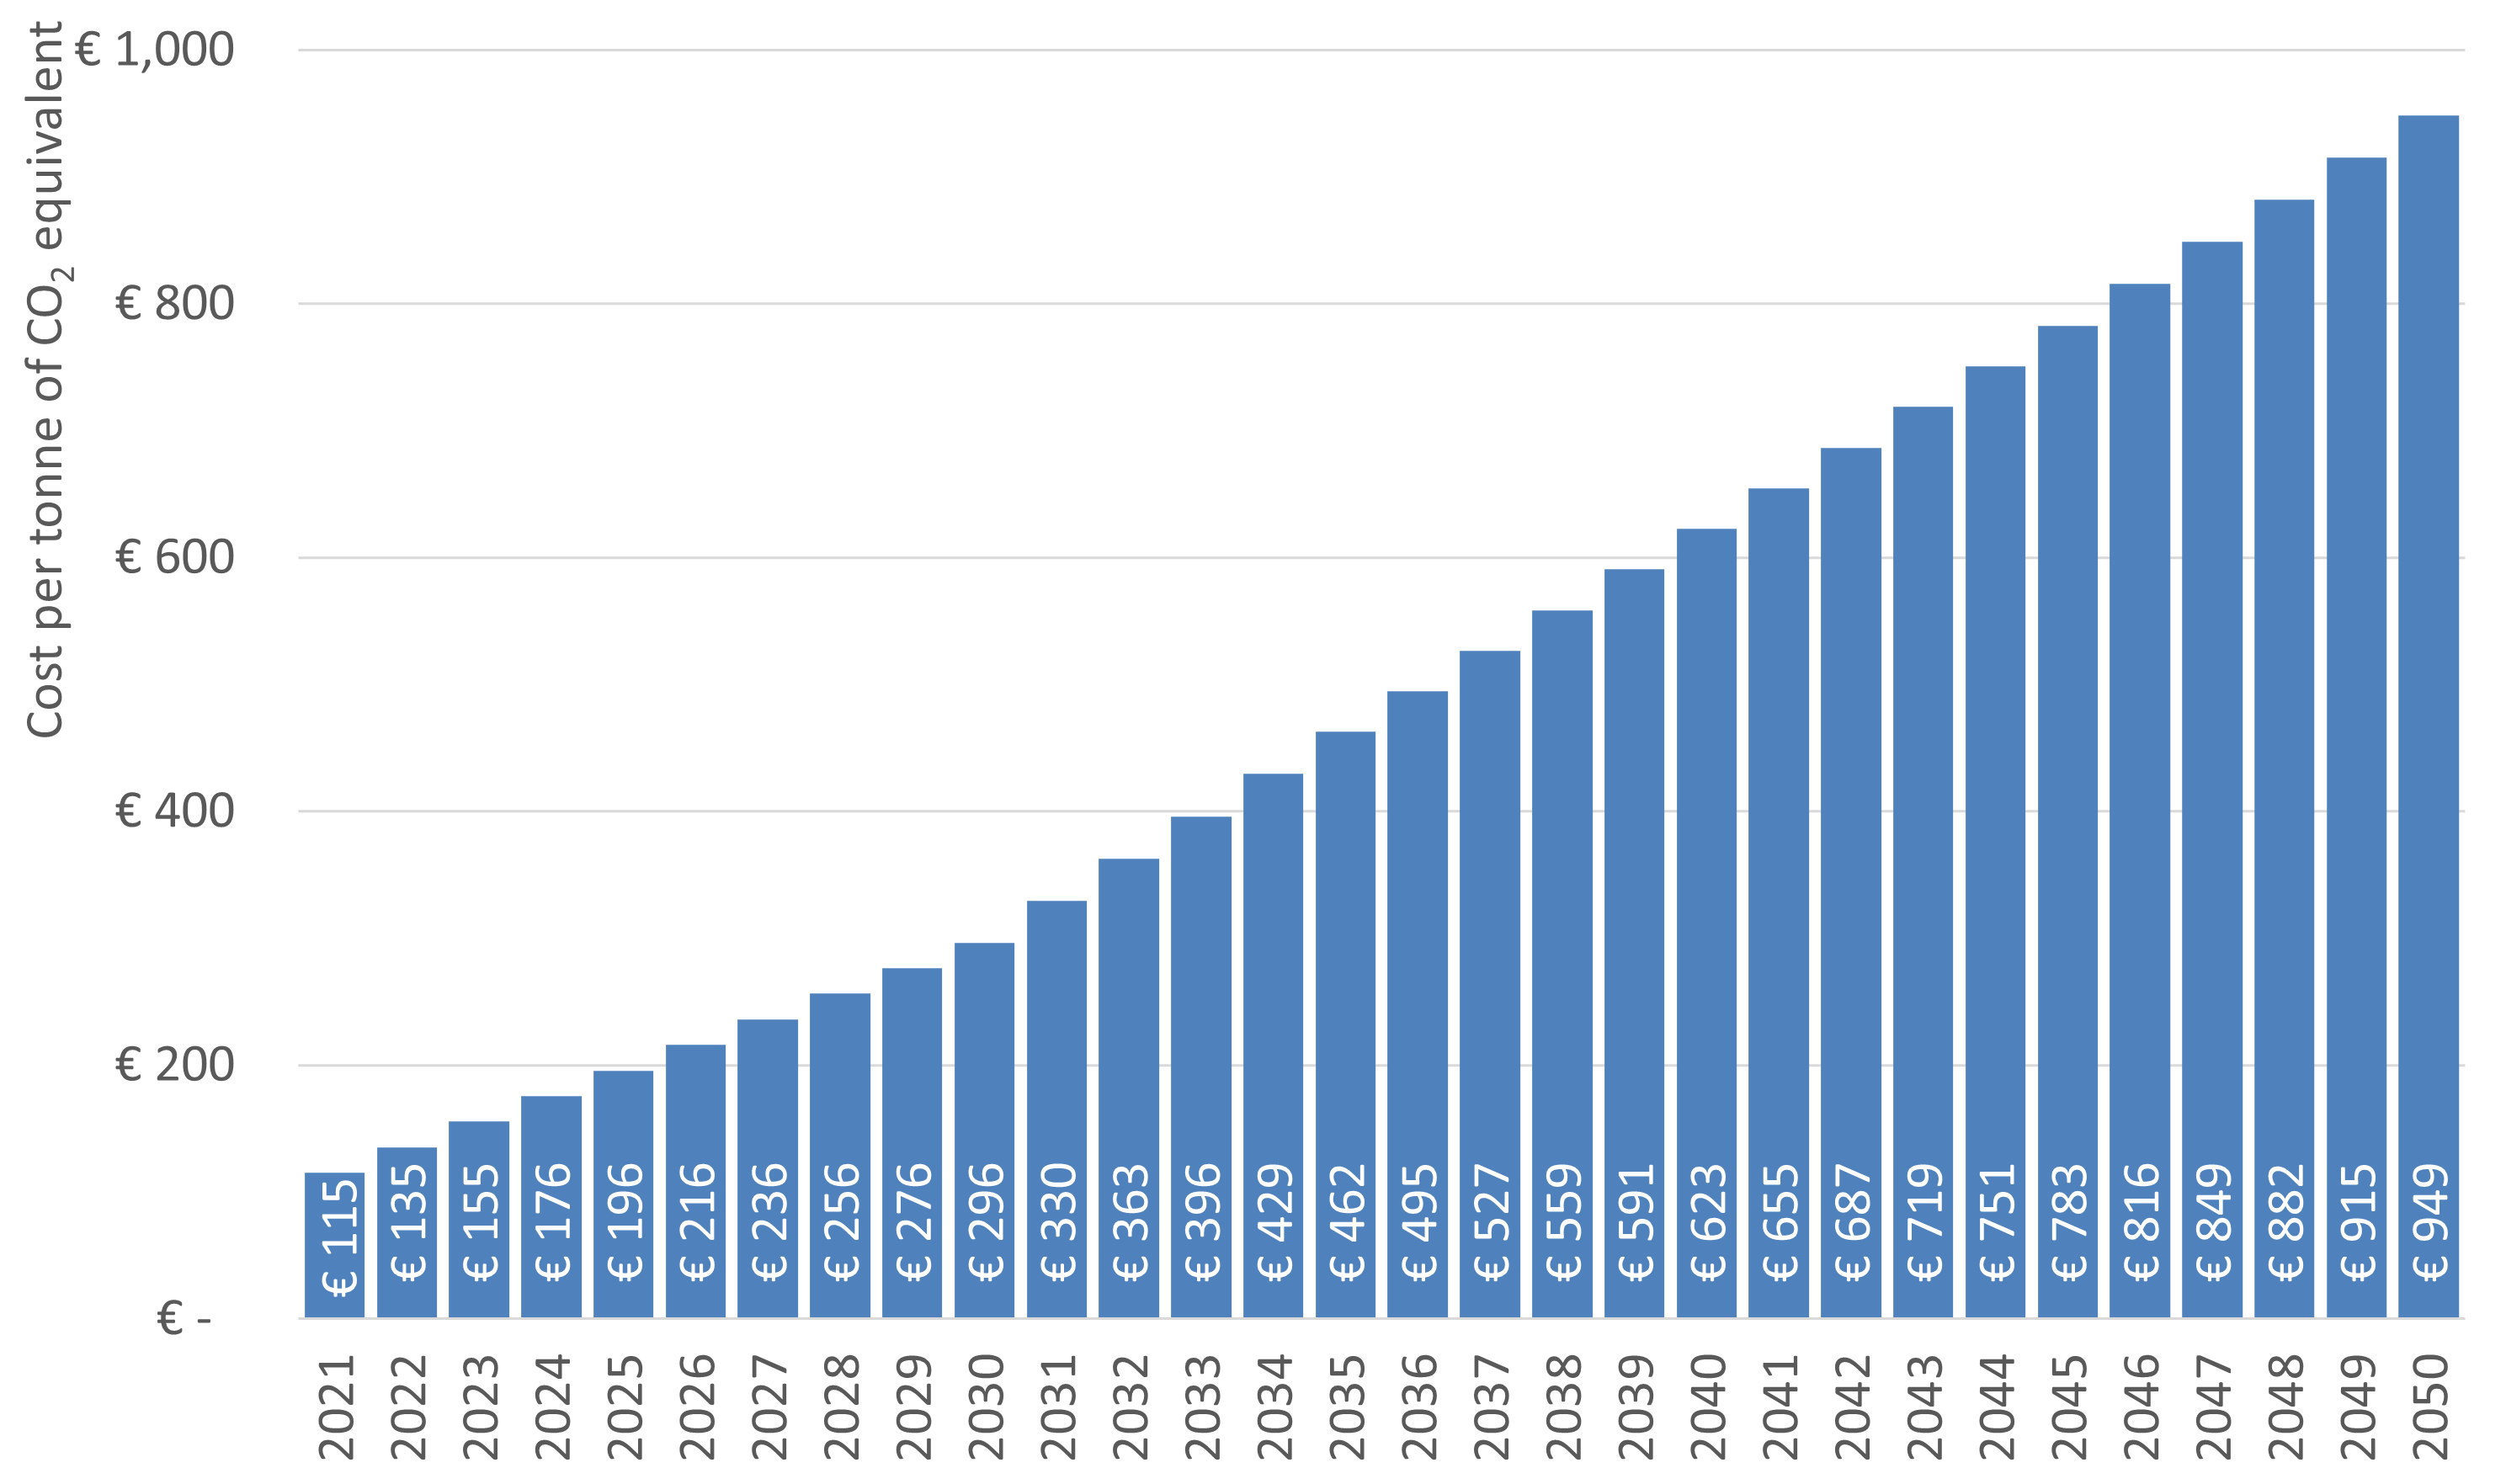
\includegraphics{./figures/cost_of_carbon.png}

}

\caption{\label{fig-cost-of-carbon}Forecast shadow cost of carbon for
EU27 in 2021 prices}

\end{figure}

\hypertarget{when-to-use-the-input-4}{%
\section{When to use the input?}\label{when-to-use-the-input-4}}

This input is recommended for projects where the full socio-economic
value of the initiative is studied, particularly involving the
environmental assessment.

\hypertarget{comments-2}{%
\section{Comments}\label{comments-2}}

In Economic Analyses the concept of `shadow cost' is often used when
working with an abstract commodity or intangible asset. Typically, two
elements are reflected in the `shadow cost':

\begin{itemize}
\tightlist
\item
  The cost of negative externalities such as pollution in this case
\item
  The shadow cost involves the consideration of future policies
\end{itemize}

Shadow costs are inexact by definition, as they are based on
assumptions, but their usefulness resides in that they help to
understand the full socio-economic merits of a project. Please note that
the shadow cost of carbon does not constitute in any way an optimal
value for any policy instrument.

\hypertarget{related-inputs-7}{%
\section{Related inputs}\label{related-inputs-7}}

\begin{itemize}
\tightlist
\item
  Chapter~\ref{sec-cost-of-emissions}
  \protect\hyperlink{sec-cost-of-emissions}{Cost of emissions}
\item
  Chapter~\ref{sec-rate-of-fuel-burn}
  \protect\hyperlink{sec-rate-of-fuel-burn}{Rate of fuel burn}
\item
  Chapter~\ref{sec-amount-of-emissions-released-by-fuel-burn}
  \protect\hyperlink{sec-amount-of-emissions-released-by-fuel-burn}{Amount
  of emissions released by fuel burn}
\item
  Chapter~\ref{sec-proportion-of-saf}
  \protect\hyperlink{sec-proportion-of-saf}{Proportion of SAF}
\end{itemize}

\hypertarget{references-8}{%
\section{References}\label{references-8}}

\hypertarget{sec-proportion-of-saf}{%
\chapter{Proportion of Sustainable Aviation
Fuel}\label{sec-proportion-of-saf}}

\hypertarget{eurocontrol-recommended-values-6}{%
\section{EUROCONTROL recommended
values}\label{eurocontrol-recommended-values-6}}

This input represents the expected evolution in the proportion of
Sustainable Aviation Fuel (SAF) in the total fuel blend between 2023 and
2050. The evolution is estimated according to three scenarios:

\begin{itemize}
\item
  \textbf{Base scenario}, where a moderate traffic growth and uptake of
  SAF is assumed, in line with \emph{ReFuelEU Aviation}
  \protect\hyperlink{ref-easa:Fit55ReFuelEU}{{[}24{]}} obligations .
\item
  \textbf{High scenario}, assumed that the high availability of SAF will
  foster the quicker adoption of these fuels than outlined in the
  current regulatory requirements.
\item
  \textbf{Low scenario}, which assumes an uptake of SAF slower that
  outlined by existing regulation.
\end{itemize}

\hypertarget{tbl-saf-blend}{}
\begin{longtable}{rrrr}
\caption{\label{tbl-saf-blend}Forecast evolution of SAF blend 2023-2050 }\tabularnewline

\toprule
Year & High scenario & Base scenario & Low scenario \\ 
\midrule
$2023$ & $1.4\%$ & $1.0\%$ & $0.8\%$ \\ 
$2024$ & $2.1\%$ & $1.5\%$ & $1.2\%$ \\ 
$2025$ & $2.8\%$ & $2.0\%$ & $1.6\%$ \\ 
$2026$ & $4.2\%$ & $2.6\%$ & $2.1\%$ \\ 
$2027$ & $5.7\%$ & $3.2\%$ & $2.6\%$ \\ 
$2028$ & $7.1\%$ & $3.8\%$ & $3.0\%$ \\ 
$2029$ & $8.6\%$ & $4.4\%$ & $3.5\%$ \\ 
$2030$ & $10.0\%$ & $5.0\%$ & $4.0\%$ \\ 
$2035$ & $29.6\%$ & $20.0\%$ & $16.0\%$ \\ 
$2040$ & $49.1\%$ & $32.0\%$ & $25.6\%$ \\ 
$2045$ & $68.7\%$ & $38.0\%$ & $30.4\%$ \\ 
$2050$ & $88.2\%$ & $63.0\%$ & $50.4\%$ \\ 
\bottomrule
\end{longtable}

\emph{Source: EUROCONTROL (2022), Objective Skygreen 2022-2030. The
economics of aviation decarbonisation towards the 2030 Green Deal
milestone} \protect\hyperlink{ref-skygreen2022}{{[}25{]}}

\hypertarget{description-1}{%
\section{Description}\label{description-1}}

Table~\ref{tbl-saf-blend} shows the forecast SAF blending percentage
over total jet fuel for years 2023 to 2050. The values are provided
based on the 3 forecast scenarios proposed by EUROCONTROL Aviation
Outlook \protect\hyperlink{ref-aviation:outlook2022}{{[}6{]}}.

The percentages of SAF are based on:

\begin{itemize}
\tightlist
\item
  The series starting with a projection of the 2022 actual SAF blending.
\item
  A linear interpolation, until in 2030 the required 5\% of the ReFuelEU
  Aviation proposal is met, followed by the same linear growth until
  2050.
\end{itemize}

Other underlying assumptions worth mentioning are:

\begin{itemize}
\tightlist
\item
  The regulation imposes obligations only on the fuel suppliers, not on
  the airlines.
\item
  Objective Skygreen 2022-2030
  \protect\hyperlink{ref-skygreen2022}{{[}25{]}} assumes that the SAF
  blending percentages apply to all the airports within the Network
  Manager area (see Figure~\ref{fig-ecac-airspace-fir}).
\end{itemize}

The figure below depicts the expected SAF blending percentages. Points
are the yearly percentages expected and the dotted line is a trend line
adjustment.

\begin{figure}

{\centering 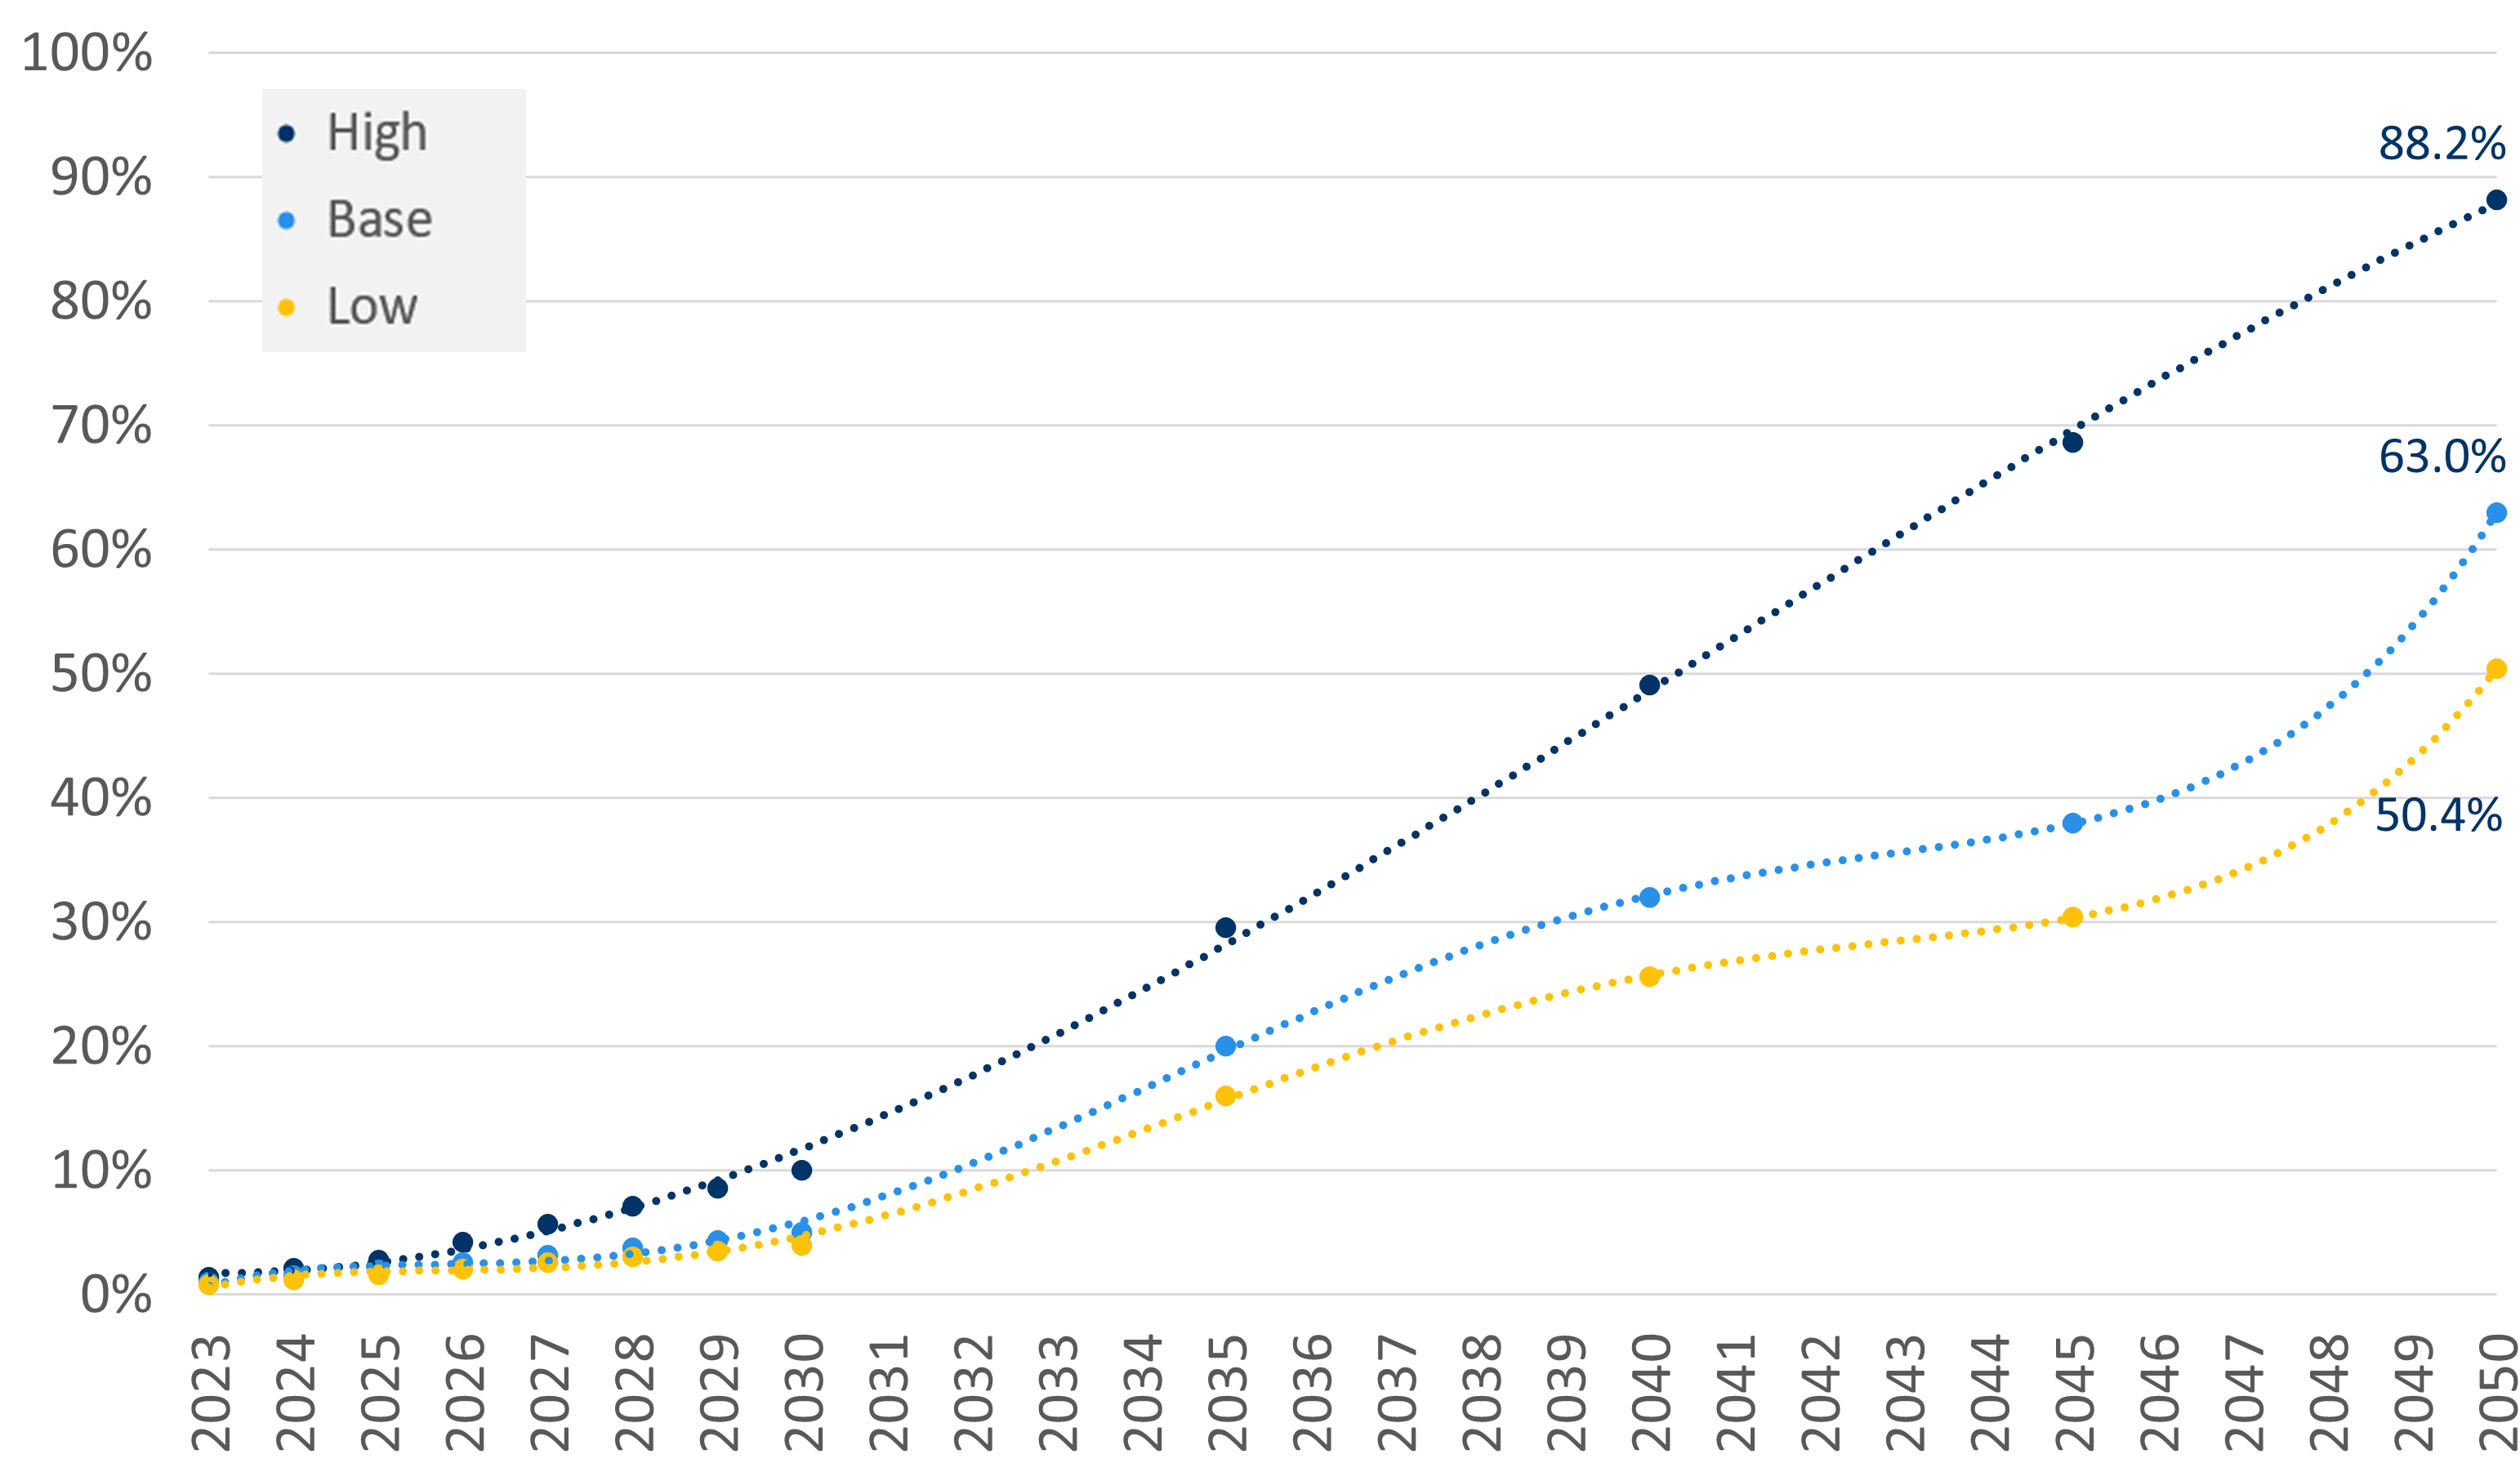
\includegraphics{./figures/saf_blend.png}

}

\caption{\label{fig-saf-blend}Forecast evolution of SAF proportion
2023-2050 \protect\hyperlink{ref-skygreen2022}{{[}25{]}}}

\end{figure}

\hypertarget{when-to-use-the-input-5}{%
\section{When to use the input?}\label{when-to-use-the-input-5}}

This input is recommended to be used when dealing with environmentally
related assessments. This data has previously been used for the traffic
forecast in EUROCONTROL Aviation Outlook 2050
\protect\hyperlink{ref-aviation:outlook2022}{{[}6{]}} and for the
Objective Skygreen study \protect\hyperlink{ref-skygreen2022}{{[}25{]}},
guiding on long-term aviation sustainability.

\hypertarget{comments-3}{%
\section{Comments}\label{comments-3}}

Non-conventional fuels -- SAF are non-fossil derived -- can be used in
aviation if blended with conventional kerosene. Many experts agree that
this is the most promising option to reduce aviation emissions in the
short to medium term.

The ReFuelEU Aviation initiative -- put forward by the European
Commission in the Fit for 55 package -- imposes a mandate on fuel
suppliers to provide SAF in jet fuel available in EU airports. The
proposal defines a series of percentages of SAF blending that will have
to be met at specific years.

For further research, please visit the work of the EUROCONTROL Aviation
Sustainability Unit \protect\hyperlink{ref-ectl:asu}{{[}26{]}}.

\hypertarget{related-inputs-8}{%
\section{Related inputs}\label{related-inputs-8}}

\begin{itemize}
\tightlist
\item
  Chapter~\ref{sec-rate-of-fuel-burn}
  \protect\hyperlink{sec-rate-of-fuel-burn}{Rate of fuel burn}
\item
  Chapter~\ref{sec-amount-of-emissions-released-by-fuel-burn}
  \protect\hyperlink{sec-amount-of-emissions-released-by-fuel-burn}{Amount
  of emissions released by fuel burn}
\item
  Chapter~\ref{sec-cost-of-emissions}
  \protect\hyperlink{sec-cost-of-emissions}{Cost of emissions}
\item
  Chapter~\ref{sec-shadow-cost-of-carbon}
  \protect\hyperlink{sec-shadow-cost-of-carbon}{Shadow cost of carbon}
\end{itemize}

\hypertarget{references-9}{%
\section{References}\label{references-9}}

\part{Airspace Users}

\hypertarget{sec-aircraft-operating-costs}{%
\chapter{Aircraft Operating Costs}\label{sec-aircraft-operating-costs}}

This chapter is being updated.

For the latest officially published version, please refer to
\href{https://www.eurocontrol.int/sites/default/files/2021-03/eurocontrol-standard-inputs-economic-analysis-ed-9.pdf}{EUROCONTROL
Standard Inputs for Economic Analyses - Edition 9}

\hypertarget{sec-average-number-of-passengers}{%
\chapter{Average number of
passengers}\label{sec-average-number-of-passengers}}

\hypertarget{eurocontrol-recommended-values-7}{%
\section{EUROCONTROL recommended
values}\label{eurocontrol-recommended-values-7}}

Figure~\ref{fig-number-of-passengers} presents an overview of the total
and average number of passengers per flight in ECAC
\protect\hyperlink{ref-ectrl:statfor:sid}{{[}5{]}}.

\begin{figure}

{\centering \includegraphics{./figures/number_passengers.png}

}

\caption{\label{fig-number-of-passengers}Number of passengers per flight
in ECAC 2012-2021 \protect\hyperlink{ref-ectrl:statfor:sid}{{[}5{]}}}

\end{figure}

\hypertarget{when-to-use-the-input-6}{%
\section{When to use the input?}\label{when-to-use-the-input-6}}

This input is suitable to be used in any analysis that requires
historical data on the number of passengers per flight and/or per
movement.

\hypertarget{comment-1}{%
\section{Comment}\label{comment-1}}

The Eurostat air transport domain contains national and international
intra- and extra-EU data. This provides air transport data for
passengers (in numbers of passengers) and for freight and mail (in
thousands of tonnes), as well as air traffic data for airports, airlines
and aircraft. Data are transmitted to Eurostat by the Member States of
the European Union as well as the candidate countries Iceland, Norway
and Switzerland. The air transport data have been calculated using data
collected at airports.

The average number of passengers per movement\footnote{A movement is
  either a take-off or a landing at an airport.} for a given year is
obtained by dividing the number of `departing passengers on board' by
the number of `departing flights for that year'.

\hypertarget{related-inputs-9}{%
\section{Related inputs}\label{related-inputs-9}}

\begin{itemize}
\tightlist
\item
  Chapter~\ref{sec-number-of-ifr-flights}
  \protect\hyperlink{sec-number-of-ifr-flights}{Number of IFR flights}
\end{itemize}

\hypertarget{references-10}{%
\section{References}\label{references-10}}

\hypertarget{sec-cancellation-cost}{%
\chapter{Cancellation Cost}\label{sec-cancellation-cost}}

This chapter is being updated.

For the latest officially published version, please refer to
\href{https://www.eurocontrol.int/sites/default/files/2021-03/eurocontrol-standard-inputs-economic-analysis-ed-9.pdf}{EUROCONTROL
Standard Inputs for Economic Analyses - Edition 9}

\hypertarget{sec-operational-cancellation-rate}{%
\chapter{Operational Cancellation
Rate}\label{sec-operational-cancellation-rate}}

This chapter is being updated.

For the latest officially published version, please refer to
\href{https://www.eurocontrol.int/sites/default/files/2021-03/eurocontrol-standard-inputs-economic-analysis-ed-9.pdf}{EUROCONTROL
Standard Inputs for Economic Analyses - Edition 9}

\hypertarget{sec-cost-of-delay}{%
\chapter{Cost of Delay}\label{sec-cost-of-delay}}

This chapter is being updated.

For the latest officially published version, please refer to
\href{https://www.eurocontrol.int/sites/default/files/2021-03/eurocontrol-standard-inputs-economic-analysis-ed-9.pdf}{EUROCONTROL
Standard Inputs for Economic Analyses - Edition 9}

\hypertarget{sec-cost-of-diversions}{%
\chapter{Cost of diversion}\label{sec-cost-of-diversions}}

This chapter is being updated.

For the latest officially published version, please refer to
\href{https://www.eurocontrol.int/sites/default/files/2021-03/eurocontrol-standard-inputs-economic-analysis-ed-9.pdf}{EUROCONTROL
Standard Inputs for Economic Analyses - Edition 9}

\hypertarget{sec-turnaround-time}{%
\chapter{Turnaround time}\label{sec-turnaround-time}}

This chapter is being updated.

For the latest officially published version, please refer to
\href{https://www.eurocontrol.int/sites/default/files/2021-03/eurocontrol-standard-inputs-economic-analysis-ed-9.pdf}{EUROCONTROL
Standard Inputs for Economic Analyses - Edition 9}

\hypertarget{sec-if-average-flight-distance-and-flight-duration}{%
\chapter{IFR average flight distance and flight
duration}\label{sec-if-average-flight-distance-and-flight-duration}}

\hypertarget{eurocontrol-recommended-values-8}{%
\section{EUROCONTROL recommended
values}\label{eurocontrol-recommended-values-8}}

The table below presents an overview of the average flight distance in
ECAC region, as well as the average flight time in the same region for
the period 2017-2021.

The data below was obtained by dividing the total distance actually
flown and the total yearly IFR flight hours respectively by the yearly
number of IFR flights in the ECAC airspace.

Please note that the numbers for 2020 and 2021 are considerably lower
due to the effect of pandemic.

\hypertarget{tbl-avg-flight-distance-duration}{}
\setlength{\LTpost}{0mm}
\begin{longtable}{rrrr}
\caption{\label{tbl-avg-flight-distance-duration}Average IFR flight distance and duration in ECAC }\tabularnewline

\toprule
Year & Distance in km & Distance in NM & Flight time in min \\ 
\midrule
2017 & $1,197$ & 646 & 98.4 \\ 
2018 & $1,209$ & 653 & 100.1 \\ 
2019 & $1,220$ & 659 & 101.3 \\ 
2020 & $510$ & 275 & 97.5 \\ 
2021 & $661$ & 357 & 100.0 \\ 
\bottomrule
\end{longtable}
\begin{minipage}{\linewidth}
\emph{Source: \href{https://www.eurocontrol.int/publication/performance-review-report-prr-2021}{EUROCONTROL (2022) Performance Review Report (PRR) 2021}; \href{https://www.eurocontrol.int/publication/performance-review-report-prr-2020}{EUROCONTROL (2022) Performance Review Report (PRR) 2020}; \href{https://ext.eurocontrol.int/analytics/saw.dll?Dashboard}{STATFOR Interactive Dashboard}}\\
\end{minipage}

With regard to flight distance,
Figure~\ref{fig-traffic-demand-distribution} illustrates that nearly
90\% of IFR flight distances for flights arriving or departing within
the Network Manager area (excl. overflights) are less than 1,000NM long.

\begin{figure}

{\centering 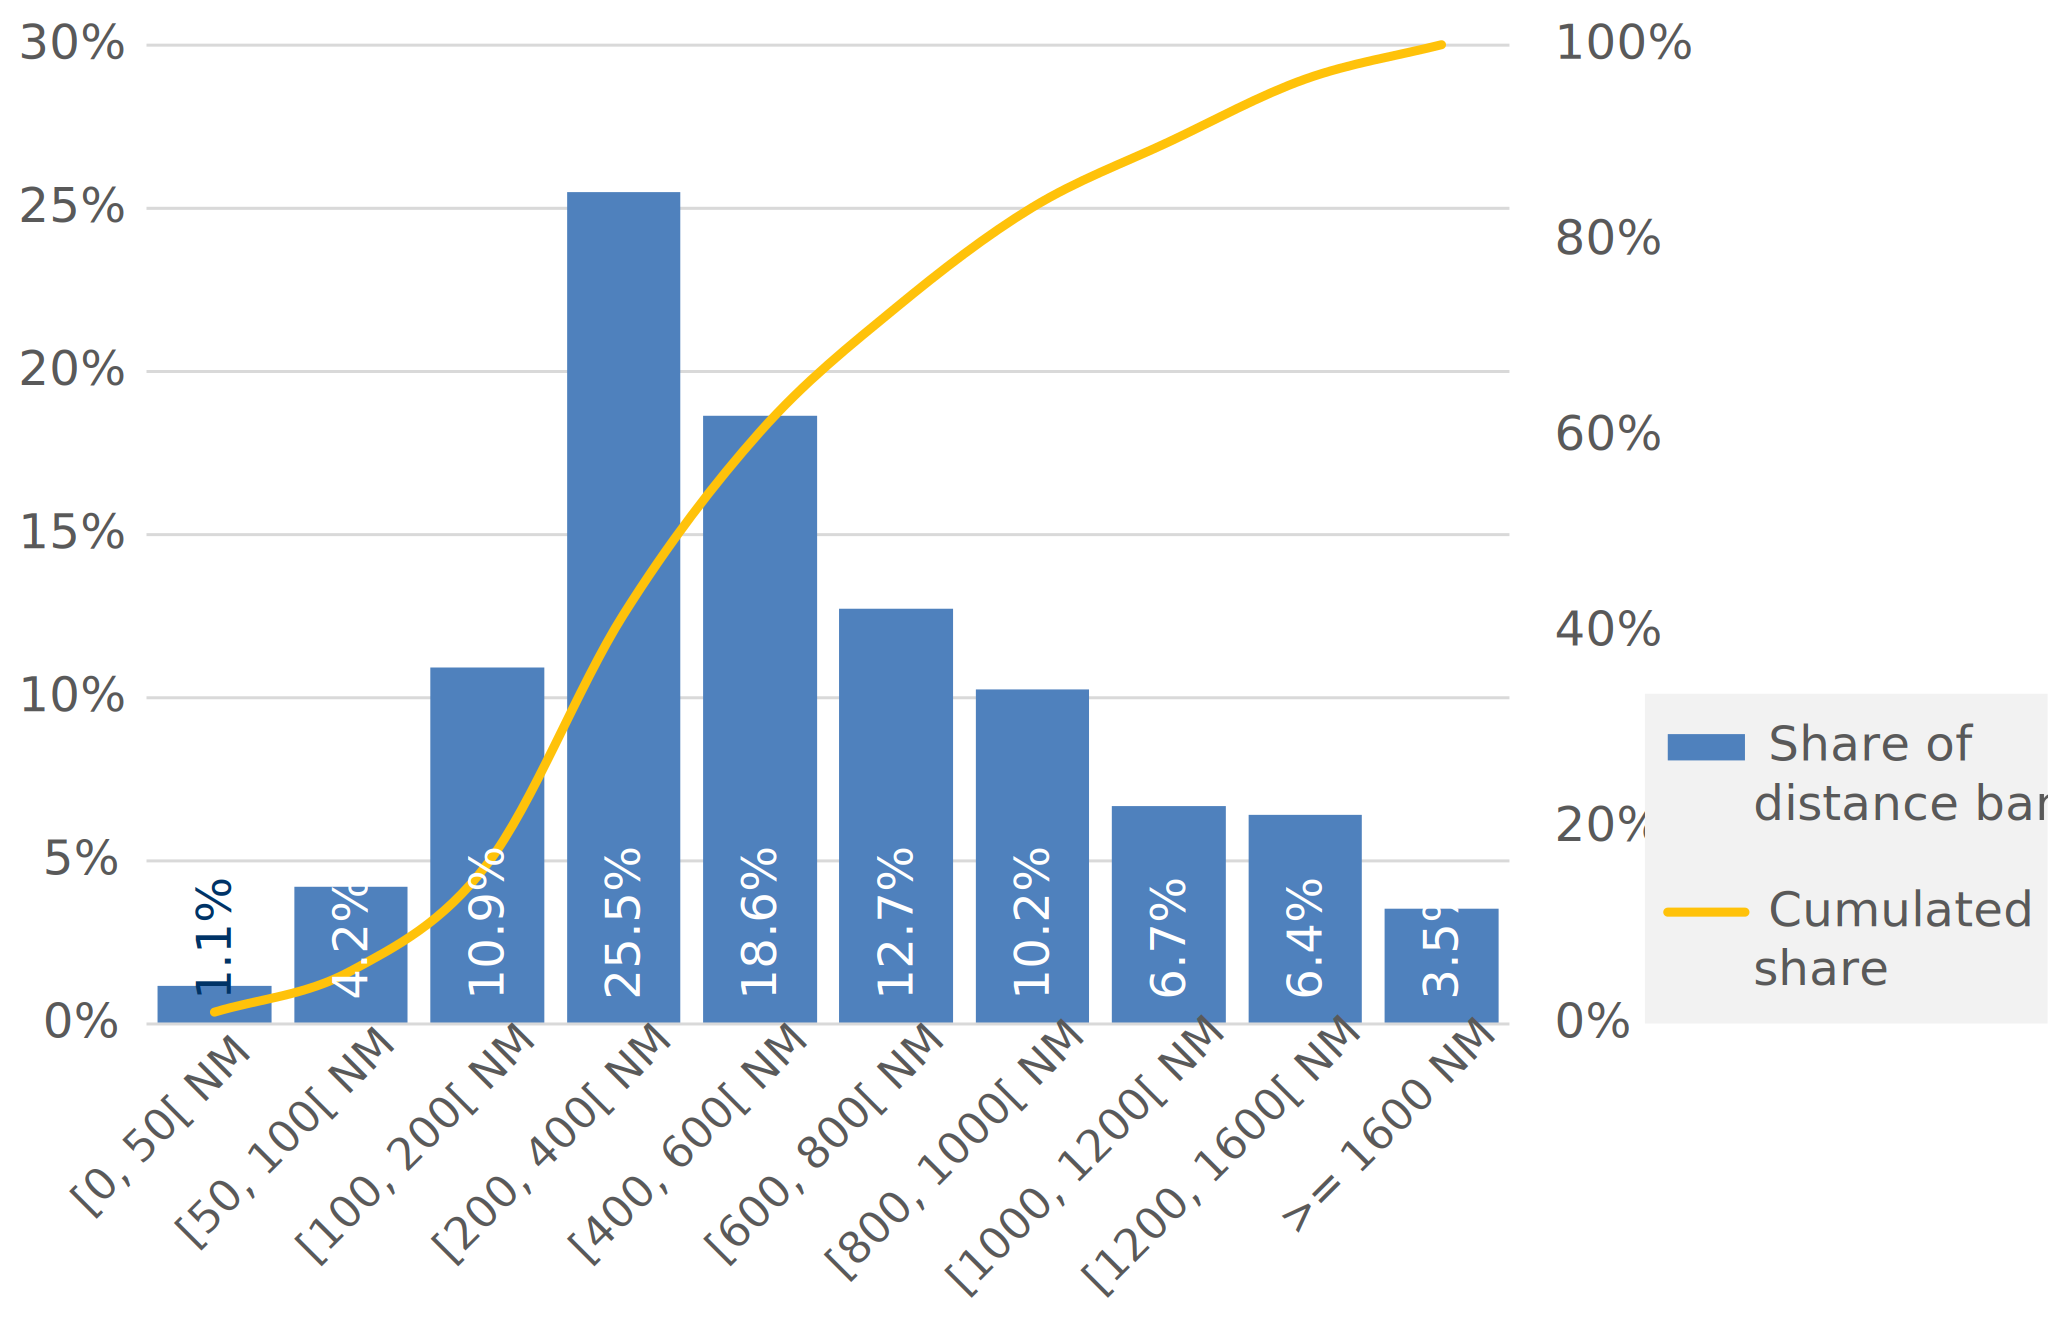
\includegraphics{./figures/traffic_demand_distribution.svg}

}

\caption{\label{fig-traffic-demand-distribution}Distribution of traffic
demand per distance band in 2022 within the EUROCONTROL Network Manager
area}

\end{figure}

\hypertarget{related-inputs-10}{%
\section{Related inputs}\label{related-inputs-10}}

\begin{itemize}
\tightlist
\item
  Chapter~\ref{sec-ifr-flight-information-per-market-segment}
  \protect\hyperlink{sec-ifr-flight-information-per-market-segment}{IFR
  flight information per market segment}
\item
  Chapter~\ref{sec-distance-flown-by-charging-zone}
  \protect\hyperlink{sec-distance-flown-by-charging-zone}{DIstance flown
  by charging zone}
\item
  Chapter~\ref{sec-taxiing-times}
  \protect\hyperlink{sec-taxiing-time}{Taxiing time}
\end{itemize}

\hypertarget{sec-ifr-flight-information-per-market-segment}{%
\chapter{IFR flight information per market
segment}\label{sec-ifr-flight-information-per-market-segment}}

This chapter is being updated.

For the latest officially published version, please refer to
\href{https://www.eurocontrol.int/sites/default/files/2021-03/eurocontrol-standard-inputs-economic-analysis-ed-9.pdf}{EUROCONTROL
Standard Inputs for Economic Analyses - Edition 9}

\hypertarget{sec-distance-flown-by-charging-zone}{%
\chapter{Distance flown by charging
zone}\label{sec-distance-flown-by-charging-zone}}

This value presents the number of kilometers flown by charging zone.

\hypertarget{tbl-distance-per-charging-zone}{}
\setlength{\LTpost}{0mm}
\begin{longtable}{lrrrrrrrrr}
\caption{\label{tbl-distance-per-charging-zone}Distance flown per charging zone in million km }\tabularnewline

\toprule
Charging zone & 2014 & 2015 & 2016 & 2017 & 2018 & 2019 & 2020 & 2021 & 2022 \\ 
\midrule
Albania & $33$ & $34$ & $31$ & $32$ & $34$ & $36$ & $16$ & $24$ & $38$ \\ 
Armenia & $9$ & $7$ & $7$ & $10$ & $13$ & $12$ & $3$ & $5$ & $11$ \\ 
Austria & $202$ & $204$ & $204$ & $219$ & $235$ & $244$ & $109$ & $135$ & $232$ \\ 
Belgium-Luxembourg & $175$ & $181$ & $183$ & $189$ & $193$ & $187$ & $75$ & $82$ & $149$ \\ 
Bosnia and Herzegovina & $59$ & $64$ & $63$ & $74$ & $79$ & $88$ & $41$ & $55$ & $90$ \\ 
Bulgaria & $174$ & $201$ & $205$ & $208$ & $233$ & $236$ & $101$ & $139$ & $231$ \\ 
Croatia & $131$ & $133$ & $131$ & $134$ & $148$ & $161$ & $66$ & $110$ & $164$ \\ 
Cyprus & $104$ & $109$ & $109$ & $123$ & $136$ & $146$ & $56$ & $84$ & $122$ \\ 
Czech Republic & $167$ & $177$ & $189$ & $193$ & $208$ & $204$ & $78$ & $90$ & $128$ \\ 
Denmark & $120$ & $123$ & $125$ & $127$ & $130$ & $133$ & $52$ & $56$ & $99$ \\ 
Finland & $58$ & $55$ & $54$ & $59$ & $65$ & $68$ & $31$ & $32$ & $46$ \\ 
France & $1,489$ & $1,514$ & $1,594$ & $1,673$ & $1,714$ & $1,729$ & $689$ & $902$ & $1,506$ \\ 
Georgia & $40$ & $41$ & $41$ & $42$ & $42$ & $37$ & $20$ & $23$ & $41$ \\ 
Germany & $990$ & $994$ & $1,029$ & $1,087$ & $1,130$ & $1,137$ & $505$ & $578$ & $951$ \\ 
Greece & $332$ & $344$ & $328$ & $364$ & $401$ & $426$ & $182$ & $275$ & $447$ \\ 
Hungary & $158$ & $173$ & $178$ & $189$ & $207$ & $202$ & $89$ & $114$ & $201$ \\ 
Ireland & $197$ & $209$ & $224$ & $224$ & $226$ & $228$ & $95$ & $115$ & $209$ \\ 
Italy & $671$ & $660$ & $671$ & $697$ & $753$ & $796$ & $321$ & $467$ & $757$ \\ 
Latvia & $54$ & $55$ & $54$ & $59$ & $63$ & $64$ & $27$ & $33$ & $34$ \\ 
Lithuania & $36$ & $35$ & $36$ & $39$ & $44$ & $45$ & $22$ & $31$ & $29$ \\ 
Malta & $41$ & $46$ & $49$ & $50$ & $52$ & $57$ & $23$ & $28$ & $38$ \\ 
Moldova & $9$ & $6$ & $5$ & $6$ & $7$ & $7$ & $3$ & $4$ & $2$ \\ 
Netherlands & $202$ & $213$ & $226$ & $232$ & $242$ & $240$ & $101$ & $106$ & $188$ \\ 
North Macedonia & $19$ & $20$ & $19$ & $23$ & $26$ & $30$ & $12$ & $20$ & $31$ \\ 
Norway & $172$ & $173$ & $181$ & $182$ & $183$ & $177$ & $94$ & $108$ & $158$ \\ 
Poland & $289$ & $288$ & $306$ & $316$ & $344$ & $360$ & $148$ & $183$ & $237$ \\ 
Portugal Lisboa & $216$ & $226$ & $252$ & $272$ & $277$ & $287$ & $112$ & $144$ & $266$ \\ 
Portugal Santa Maria & $196$ & $217$ & $236$ & $251$ & $259$ & $260$ & $117$ & $143$ & $243$ \\ 
Romania & $251$ & $266$ & $257$ & $274$ & $298$ & $299$ & $126$ & $175$ & $276$ \\ 
Serbia / Montenegro / KFOR & $133$ & $149$ & $158$ & $166$ & $186$ & $195$ & $83$ & $113$ & $194$ \\ 
Slovak Republic & $72$ & $72$ & $76$ & $79$ & $86$ & $86$ & $31$ & $41$ & $65$ \\ 
Slovenia & $37$ & $37$ & $39$ & $41$ & $44$ & $48$ & $20$ & $28$ & $45$ \\ 
Spain-Canarias & $101$ & $98$ & $106$ & $114$ & $124$ & $131$ & $356$ & $73$ & $124$ \\ 
Spain-Continental & $707$ & $725$ & $780$ & $835$ & $881$ & $909$ & $57$ & $512$ & $875$ \\ 
Sweden & $257$ & $258$ & $261$ & $276$ & $287$ & $283$ & $120$ & $129$ & $199$ \\ 
Switzerland & $120$ & $121$ & $124$ & $134$ & $144$ & $144$ & $54$ & $75$ & $127$ \\ 
Turkey & $789$ & $856$ & $853$ & $933$ & $1,021$ & $1,036$ & $460$ & $658$ & $938$ \\ 
United Kingdom & $706$ & $720$ & $768$ & $821$ & $838$ & $852$ & $335$ & $360$ & $719$ \\ 
Subtotal & $9,516$ & $9,805$ & $10,153$ & $10,748$ & $11,352$ & $11,582$ & $4,829$ & $6,250$ & $10,208$ \\ 
Estonia* & NA & NA & NA & $41$ & $56$ & $55$ & $23$ & $26$ & $29$ \\ 
Ukraine* & NA & NA & NA & NA & NA & NA & NA & NA & $12$ \\ 
Ukraine South* & NA & NA & NA & NA & NA & NA & NA & NA & $2$ \\ 
Total & $9,516$ & $9,805$ & $10,153$ & $10,789$ & $11,407$ & $11,636$ & $4,853$ & $6,279$ & $10,239$ \\ 
\bottomrule
\end{longtable}
\begin{minipage}{\linewidth}
\emph{Source:EUROCONTROL Central Route Charges Office -- Draft Internal data for 2022 and \href{https://www.eurocontrol.int/publication/report-operation-route-charges-system-2021}{Report on the Operation of the Route Charges System in 2021}}\\
\end{minipage}

Please note that data for Estonia and Ukraine is not available from the
beginning because these countries integrated in April 2017 and November
2021 respectively.

For the most updated information, the
\href{https://www.eurocontrol.int/ServiceUnits/Dashboard/EnRouteMainDashboard.html}{Aviation
Intelligence En Route Dashboard} can be accessed.

\hypertarget{description-2}{%
\section{Description}\label{description-2}}

The Report on the Operation of the Route Charges System is published by
the CRCO on an annual basis and provides data on traffic volumes and ATM
costs for the States for which the CRCO collects en route and terminal
charges.

Table~\ref{tbl-distance-per-charging-zone} sets out the number of
millions of kilometers recorded in the airspace of the Contracting
States from 2014 to 2022 for the calculation of route charges (great
circle distance after deduction of 20 km for departing and arriving
flights) as well as the average annual variation observed during the
same period.

Information on the various different charges levied by the CRCO, in
particular the charge calculation methods, the basic billing documents,
the methods of payment and the submission of claims is described in
\href{https://www.eurocontrol.int/publication/customer-guide-route-charges}{Customer
Guide to Charges}.

\hypertarget{related-inputs-11}{%
\section{Related inputs}\label{related-inputs-11}}

\begin{itemize}
\item
  Chapter~\ref{sec-if-average-flight-distance-and-flight-duration}
  \protect\hyperlink{sec-if-average-flight-distance-and-flight-duration}{IFR
  average flight distance and flight duration}
\item
  Chapter~\ref{sec-en-route-ans-costs}
  \protect\hyperlink{sec-en-route-ans-costs}{En-route ANS costs}
\item
  Chapter~\ref{sec-route-charge-share-per-market-segment}
  \protect\hyperlink{sec-route-charge-share-per-market-segment}{Route
  charge share per market segment}
\end{itemize}

\hypertarget{sec-load-factor-cargo}{%
\chapter{Load factor -- cargo}\label{sec-load-factor-cargo}}

This chapter is being updated.

For the latest officially published version, please refer to
\href{https://www.eurocontrol.int/sites/default/files/2021-03/eurocontrol-standard-inputs-economic-analysis-ed-9.pdf}{EUROCONTROL
Standard Inputs for Economic Analyses - Edition 9}

\hypertarget{sec-load-factor-passengers}{%
\chapter{Load factor -- passengers}\label{sec-load-factor-passengers}}

This chapter is being updated.

For the latest officially published version, please refer to
\href{https://www.eurocontrol.int/sites/default/files/2021-03/eurocontrol-standard-inputs-economic-analysis-ed-9.pdf}{EUROCONTROL
Standard Inputs for Economic Analyses - Edition 9}

\hypertarget{sec-cost-of-aviation-fuel}{%
\chapter{Cost of aviation fuel}\label{sec-cost-of-aviation-fuel}}

\hypertarget{eurocontrol-recommended-sources-1}{%
\section{EUROCONTROL recommended
sources}\label{eurocontrol-recommended-sources-1}}

The source recommended to consult for the latest data on the cost of
aviation fuel is
\href{https://eurocontrol.sharepoint.com/sites/ECTL-Business_Cases/Shared\%20Documents/Standard_Inputs/1.\%20NEW_2022/Values/Cost\%20of\%20aviation\%20fuel/IATA\%20Jet\%20Fuel\%20Price\%20Monitor}{IATA
Jet Fuel Price Monitor}.

On its website, IATA provides jet fuel prices for the major regions of
the world, together with analysis and commentary. The values are based
on \href{http://www.platts.com/}{Platts Energy Market Data}.

When estimating the jet fuel price, consideration should be given to the
selection of the geographical area, and hence currency, as a change in
oil price can have a different effect on the jet fuel price owing to
currency fluctuations, e.g.~the downturn in the euro in 2015.

The `spread' between the aviation fuel price and the underlying oil
price covers the cost of refining, but it can vary significantly with
time depending on underlying demand (e.g.~from consumers needing a
similar fraction to aviation), and on supply problems (such as a
breakdown at a refinery or increasing local prices relative to oil).

\hypertarget{other-possible-sources}{%
\section{Other possible sources}\label{other-possible-sources}}

Other sources that may be interesting to consult to estimate the price
of jet fuel include:

\begin{itemize}
\item
  \href{https://www.iata.org/en/publications/economics/?Search=\&EconomicsL1=149\&EconomicsL2=150\#searchForm}{IATA
  Airline Industry Economic Performance Report and Tables}
\item
  \href{http://www.eia.gov/forecasts/aeo/}{US Energy Information
  Administration (2022), Annual Energy Outlook 2022}
\end{itemize}

\hypertarget{sec-value-of-an-average-passenger-flight}{%
\chapter{Value of an average passenger
flight}\label{sec-value-of-an-average-passenger-flight}}

\hypertarget{eurocontrol-recommended-values-9}{%
\section{EUROCONTROL recommended
values}\label{eurocontrol-recommended-values-9}}

This value represents the monetised benefits of an average passenger
flight in the EU27. The values were adjusted to 2022 price levels based
on inflation.

\hypertarget{tbl-value-of-passenger-flight}{}
\setlength{\LTpost}{0mm}
\begin{longtable}{lrr}
\caption{\label{tbl-value-of-passenger-flight}Value of an average passenger flight }\tabularnewline

\toprule
  & International flight & Domestic flight \\ 
\midrule
Consumer benefits per flight & $\text{EUR}27,636$ & $\text{EUR}5,070$ \\ 
Airline benefits per flight (excl. fuel and labour) & $\text{EUR}829$ & $\text{EUR}149$ \\ 
Other producer benefits per flight (excl. fuel and labour) & $\text{EUR}1,493$ & $\text{EUR}739$ \\ 
\bottomrule
\end{longtable}
\begin{minipage}{\linewidth}
\emph{Source: \href{https://www.iata.org/en/iata-repository/publications/economic-reports/value-of-an-average-passenger-flight-in-eu-27/}{IATA (2013). Economic Briefing - The value of an average passenger flight in the EU27}}\\
\end{minipage}

\textbf{Consumer benefits} are the benefits for passengers, calculated
based on the difference between the consumer's willingness to pay (or
the gross consumer benefit) and the price paid.

\textbf{Producer benefits} are assessed from the investors' perspective,
relying on profitability measures such as return on invested capital
(ROIC). ROIC is calculated before payments of debt interest and shows
the earnings available to pay both debt and equity investors.
Furthermore, the calculation excludes fuel and labour related benefits.
The estimated profits of the fuel supply chain round € 11-35 billion per
year globally. The vast majority of these profits are allocated with the
crude oil suppliers.

\textbf{Wider economic benefits} represent those that go beyond the
direct impact on the users, such as any spillover effects from in
increased competition and more efficient movement of capital and labour.

One of the largest economic benefits of increased connectivity comes
from its impact on the long term productivity of the wider economy.
There are several approaches which may be used to quantify this benefit.
One conservative approach which has been developed, on the basis of the
statistical relationship between air connectivity and labour
productivity, yields an estimate that a \textbf{10\% rise in
connectivity, relative to a country's GDP, will boost labour
productivity levels by 0.07\%.}

\hypertarget{when-to-use-the-input-7}{%
\section{When to use the input?}\label{when-to-use-the-input-7}}

The use of these values depends on the scope and the viewpoint of the
analysis. For example, an assessment from the point of view of airlines
will focus on the benefits that an additional flight brings to airlines,
whereas an analysis from the perspective of a government or the European
Commission should also include an assessment of benefits for consumers
and the wider economy.

Note also that these values reflect the market conditions and the
passenger demand at the time of the study. For example, changes in
passengers' income, changes in their preferences for air transport or
changes in airlines' market structure can affect these values.

\hypertarget{sec-fleet-age}{%
\chapter{Fleet age}\label{sec-fleet-age}}

This chapter is being updated.

For the latest officially published version, please refer to
\href{https://www.eurocontrol.int/sites/default/files/2021-03/eurocontrol-standard-inputs-economic-analysis-ed-9.pdf}{EUROCONTROL
Standard Inputs for Economic Analyses - Edition 9}

\hypertarget{sec-fleet-size}{%
\chapter{Fleet size}\label{sec-fleet-size}}

This chapter is being updated.

For the latest officially published version, please refer to
\href{https://www.eurocontrol.int/sites/default/files/2021-03/eurocontrol-standard-inputs-economic-analysis-ed-9.pdf}{EUROCONTROL
Standard Inputs for Economic Analyses - Edition 9}

\hypertarget{sec-fleet-cns-capability}{%
\chapter{Fleet CNS capability}\label{sec-fleet-cns-capability}}

This chapter is being updated.

For the latest officially published version, please refer to
\href{https://www.eurocontrol.int/sites/default/files/2021-03/eurocontrol-standard-inputs-economic-analysis-ed-9.pdf}{EUROCONTROL
Standard Inputs for Economic Analyses - Edition 9}

\part{ATM}

\hypertarget{sec-en-route-ans-costs}{%
\chapter{En-route ANS costs}\label{sec-en-route-ans-costs}}

\hypertarget{eurocontrol-recommended-values-10}{%
\section{EUROCONTROL recommended
values}\label{eurocontrol-recommended-values-10}}

This input represents the costs of Air Navigation Services (ANS) in
en-route airspace that is under the control of States/ANSPs.

Table~\ref{tbl-ans-costs} shows the \textbf{real en-route ANS cost per
TSU for EUROCONTROL area.} The values refer to 2020 and are presented
\textbf{in million euros}.

\hypertarget{tbl-ans-costs}{}
\setlength{\LTpost}{0mm}
\begin{longtable}{lrrrrrr}
\caption{\label{tbl-ans-costs}En-route ANS costs }\tabularnewline

\toprule
  & 2015 & 2016 & 2017 & 2018 & 2019 & 2020 \\ 
\midrule
SES states (EU27+3)\textsuperscript{1} & $\text{EUR}6,225$ & $\text{EUR}6,201$ & $\text{EUR}6,167$ & $\text{EUR}6,235$ & $\text{EUR}6,307$ & $\text{EUR}6,136$ \\ 
Other 10 States in the Route Charges System\textsuperscript{2} & $\text{EUR}1,247$ & $\text{EUR}1,287$ & $\text{EUR}1,282$ & $\text{EUR}1,348$ & $\text{EUR}1,380$ & $\text{EUR}1,412$ \\ 
Total en-route ANS costs & $\text{EUR}7,472$ & $\text{EUR}7,488$ & $\text{EUR}7,449$ & $\text{EUR}7,583$ & $\text{EUR}7,687$ & $\text{EUR}7,548$ \\ 
SES states (EU27+3) & 105 & 109 & 115 & 122 & 125 & 53 \\ 
Other 9 States in the Route Charges System & 29 & 30 & 33 & 35 & 36 & 16 \\ 
Total en-route service units (million TSU) & 134 & 139 & 148 & 157 & 161 & 69 \\ 
SES states (EU27+3) & $\text{EUR}59$ & $\text{EUR}57$ & $\text{EUR}54$ & $\text{EUR}51$ & $\text{EUR}50$ & $\text{EUR}117$ \\ 
Other 9 States in the Route Charges System & $\text{EUR}43$ & $\text{EUR}43$ & $\text{EUR}39$ & $\text{EUR}38$ & $\text{EUR}38$ & $\text{EUR}90$ \\ 
Total en-route ANS costs per TSU & $\text{EUR}102$ & $\text{EUR}100$ & $\text{EUR}93$ & $\text{EUR}90$ & $\text{EUR}88$ & $\text{EUR}206$ \\ 
\bottomrule
\end{longtable}
\begin{minipage}{\linewidth}
\textsuperscript{1}SES States refer  to  EU27  plus  Switzerland and Norway\\
\textsuperscript{2}The 10 States refer to those that are not bound by SES regulation, but which were part of the EUROCONTROL Multilateral Route Charges System in 2020 (i.e. Albania, Armenia, Bosnia‐Herzegovina, Georgia, Moldova, North Macedonia, Serbia, Montenegro, United Kingdom and Türkiye)\\
\emph{Source: \href{https://www.eurocontrol.int/publication/performance-review-report-prr-202}{EUROCONTROL (2022), Perofrmance Review Report}}\\
\end{minipage}

\hypertarget{description-3}{%
\section{Description}\label{description-3}}

ANS en-route costs per Service Unit (TSU) in the above Value are
measured on the basis of the total actual and determined en-route ANS
costs (in real terms) divided by the number of en-route Service Units. A
Service Unit, used for the calculation of route charges, multiplies the
Aircraft Weight factor by the Distance factor.

\begin{tcolorbox}[enhanced jigsaw, colframe=quarto-callout-note-color-frame, colback=white, toptitle=1mm, coltitle=black, leftrule=.75mm, title=\textcolor{quarto-callout-note-color}{\faInfo}\hspace{0.5em}{Note}, left=2mm, rightrule=.15mm, bottomtitle=1mm, breakable, titlerule=0mm, arc=.35mm, colbacktitle=quarto-callout-note-color!10!white, bottomrule=.15mm, opacityback=0, opacitybacktitle=0.6, toprule=.15mm]

Please note the difference between
\href{https://ansperformance.eu/acronym/su/}{Total Service Units (TSU)}
and \href{https://ansperformance.eu/acronym/tnsu/}{Terminal Service
Units (TNSU)}.

\end{tcolorbox}

\begin{tcolorbox}[enhanced jigsaw, colframe=quarto-callout-note-color-frame, colback=white, toptitle=1mm, coltitle=black, leftrule=.75mm, title=\textcolor{quarto-callout-note-color}{\faInfo}\hspace{0.5em}{Note}, left=2mm, rightrule=.15mm, bottomtitle=1mm, breakable, titlerule=0mm, arc=.35mm, colbacktitle=quarto-callout-note-color!10!white, bottomrule=.15mm, opacityback=0, opacitybacktitle=0.6, toprule=.15mm]

The unit rate of charge is the charge in euros applied by a Charging
Zone to a flight operated by an aircraft of 50 metric tonnes (weight
factor of 1.00) and flying 100 kilometres (distance factor of 1.00) in
the charge area of that State.

Further information on calculating unit rates can be found on
\href{https://www.eurocontrol.int/publication/customer-guide-route-charges}{customer
guide to charges website}

\end{tcolorbox}

The en-route ANS determined costs for a reference period of five years
are costs pre determined by the SES States as referred to in Article
15(2)(a) of
\href{http://eur\%20lex.europa.eu/LexUriServ/LexUriServ.do?uri=CONSLEG:2004R0550:20091204:EN:PDF}{Regulation
(EC) No 550/2004}\\
for providing air navigation services. These include amounts for
interests on debt, return on equity, depreciation of assets, as well as
staff costs and non staff operating costs for maintenance, operations,
management and administration. These costs are determined on a national
level and comprise the costs of several entities (the National
Supervisory Authority, Air Navigation Service Provider(s), the MET
service provider and the State's contribution to EUROCONTROL budget).

\hypertarget{other-sources}{%
\section{Other sources}\label{other-sources}}

Other source could be the EUROCONTROL Central Route Charges Office. At
the time of writing this update of the EUROCONTROL Standard Inputs for
Economic Analyses, the most recent published version is the
\href{https://www.eurocontrol.int/publication/report-operation-route-charges-system-2021}{2021
Report on the Operation of the Route Charges System}. Please, check
regularly the
\href{https://www.eurocontrol.int/library/search?f\%5B0\%5D=activity\%3A768\&f\%5B1\%5D=topic\%3A1159\&f\%5B2\%5D=activity\%3A768\&f\%5B3\%5D=topic\%3A1159}{CRCO
full list of reports on the operation of the route charges system} for
the latest information.

The CRCO calculates route charges using flight messages sent by the
Contracting States' Route Charges Offices (CRCOs) and additional flight
information made available via the EUROCONTROL Network Management
Directorate (NMD). The CRCO bills aircraft operators on a monthly basis,
collects charges and disburses the amounts collected to the States every
week.

\hypertarget{comment-2}{%
\section{Comment}\label{comment-2}}

Terminal ANS costs and ANSP gate to gate economic performance are
described separately in chapter 6 of the EUROCONTROL Performance Review
Report \protect\hyperlink{ref-ectrlprr2022}{{[}27{]}}.

\hypertarget{related-inputs-12}{%
\section{Related inputs}\label{related-inputs-12}}

\begin{itemize}
\tightlist
\item
  Chapter~\ref{sec-distance-flown-by-charging-zone}
  \protect\hyperlink{sec-distance-flown-by-charging-zone}{Distance flown
  by charging zone}
\end{itemize}

\hypertarget{references-11}{%
\section{References}\label{references-11}}

\hypertarget{sec-route-charge-share-per-market-segment}{%
\chapter{Route charge share per market
segment}\label{sec-route-charge-share-per-market-segment}}

This chapter is being updated.

For the latest officially published version, please refer to
\href{https://www.eurocontrol.int/sites/default/files/2021-03/eurocontrol-standard-inputs-economic-analysis-ed-9.pdf}{EUROCONTROL
Standard Inputs for Economic Analyses - Edition 9}

\hypertarget{sec-ansp-employment-cost}{%
\chapter{ANSP Employment Costs}\label{sec-ansp-employment-cost}}

\hypertarget{eurocontrol-recommended-values-11}{%
\section{EUROCONTROL recommended
values}\label{eurocontrol-recommended-values-11}}

In this section are considered ANSPs' average annual employment costs
for one Full Time Equivalent (FTE) in euros by category of staff. The
table below shows the recommended values in 2020.

\hypertarget{tbl-ansp-employment-cost-general}{}
\setlength{\LTpost}{0mm}
\begin{longtable}{lrr}
\caption{\label{tbl-ansp-employment-cost-general}Average yearly ANSPs employment costs }\tabularnewline

\toprule
Staff function & EUROCONTROL area & SES area \\ 
\midrule
ATCOs in OPS & $\text{EUR}151,000$ & $\text{EUR}155,000$ \\ 
Support Staff & $\text{EUR}74,000$ & $\text{EUR}78,000$ \\ 
Average all staff & $\text{EUR}99,000$ & $\text{EUR}103,000$ \\ 
\bottomrule
\end{longtable}
\begin{minipage}{\linewidth}
\emph{Source: \href{https://ansperformance.eu/publications/prc/ace/}{EUROCONTROL (2022), ATM cost-effectiveness (ACE) benchmarking report for 2020 with 2021-2024 outlook}}\\
\end{minipage}

\hypertarget{description-4}{%
\section{Description}\label{description-4}}

One full-time equivalent (FTE) is the equivalent of a single person
carrying out a particular job or activity working on a full-time basis
during a year. A part-time employee working half-time would be counted
as 0.5 FTEs. A full-time ATCO working two thirds of her time on duty in
ops and one third of her time on teaching at a training academy would be
counted as a 0.67 FTE ATCO in ops and a 0.33 FTE ATCO on other duties.

Employment costs comprise gross wages and salaries, payment for
overtime, employer contributions to social security schemes and taxes,
pension contributions and other benefits. For a study on employment
costs, the categories of staff working in an ANSP have been divided into
two:

\begin{itemize}
\item
  \textbf{ATCOs in ops:} ATCOs participating in an activity which is
  either directly related to the control of traffic or where there is a
  necessary requirement for ATCOs to be able to control traffic
\item
  \textbf{Support staff or non-ATCO in ops:} this category includes all
  other staff. It includes ATCOs on other duties (participating in an
  activity outside ops, such as special projects, teaching at a training
  academy, providing instruction in a simulator, working in a full-time
  management position, etc.), trainees, ATC assistants, technical and
  operational support staff, administration staff, and others
\end{itemize}

The following table gives an overview of individual ANSPs and average
European system FTE costs for the two categories. The values were
calculated based on information extracted from EUROCONTROL ACE
Report\protect\hyperlink{ref-ace2020}{{[}28{]}}.

\hypertarget{tbl-ansp-employment-cost-detailed}{}
\begin{longtable}{llrrr}
\caption{\label{tbl-ansp-employment-cost-detailed}Individual ANSP and average European system FTE costs }\tabularnewline

\toprule
ANSP & State & ATCO in ops & Support staff & All staff \\ 
\midrule
Albcontrol & Albania & $\text{EUR}28,518$ & $\text{EUR}13,527$ & $\text{EUR}16,167$ \\ 
ANS CR & Czech Republic & $\text{EUR}134,614$ & $\text{EUR}53,925$ & $\text{EUR}71,273$ \\ 
ARMATS & Armenia & $\text{EUR}23,268$ & $\text{EUR}13,417$ & $\text{EUR}15,796$ \\ 
Austro Control & Austria & $\text{EUR}203,531$ & $\text{EUR}108,390$ & $\text{EUR}139,951$ \\ 
Avinor (Continental) & Norway & $\text{EUR}189,000$ & $\text{EUR}98,725$ & $\text{EUR}134,857$ \\ 
BULATSA & Bulgaria & $\text{EUR}100,669$ & $\text{EUR}44,450$ & $\text{EUR}58,723$ \\ 
Croatia Control & Croatia & $\text{EUR}127,817$ & $\text{EUR}62,620$ & $\text{EUR}84,970$ \\ 
DCAC Cyprus & Cyprus & $\text{EUR}95,163$ & $\text{EUR}60,238$ & $\text{EUR}76,030$ \\ 
DFS & Germany & $\text{EUR}251,567$ & $\text{EUR}102,683$ & $\text{EUR}151,485$ \\ 
DHMI & Turkey & $\text{EUR}56,915$ & $\text{EUR}16,146$ & $\text{EUR}25,685$ \\ 
DSNA & France & $\text{EUR}134,859$ & $\text{EUR}100,783$ & $\text{EUR}113,243$ \\ 
EANS & Estonia & $\text{EUR}119,983$ & $\text{EUR}46,356$ & $\text{EUR}70,898$ \\ 
ENAIRE & Spain & $\text{EUR}188,964$ & $\text{EUR}95,189$ & $\text{EUR}135,096$ \\ 
ENAV & Italy & $\text{EUR}147,111$ & $\text{EUR}94,598$ & $\text{EUR}119,925$ \\ 
Fintraffic ANS & Findland & $\text{EUR}124,857$ & $\text{EUR}83,327$ & $\text{EUR}102,773$ \\ 
HCAA & Greece & $\text{EUR}73,272$ & $\text{EUR}50,605$ & $\text{EUR}57,347$ \\ 
HungaroControl & Hungary & $\text{EUR}125,358$ & $\text{EUR}42,347$ & $\text{EUR}61,446$ \\ 
IAA & Ireland & $\text{EUR}152,829$ & $\text{EUR}115,258$ & $\text{EUR}134,963$ \\ 
LFV & Sweden & $\text{EUR}316,662$ & $\text{EUR}149,023$ & $\text{EUR}225,364$ \\ 
LGS & Latvia & $\text{EUR}69,452$ & $\text{EUR}31,223$ & $\text{EUR}39,265$ \\ 
LPS & Slovak Republic & $\text{EUR}125,745$ & $\text{EUR}41,917$ & $\text{EUR}59,439$ \\ 
LVNL & Netherlands & $\text{EUR}171,593$ & $\text{EUR}132,778$ & $\text{EUR}140,021$ \\ 
MATS & Malta & $\text{EUR}103,766$ & $\text{EUR}53,389$ & $\text{EUR}68,188$ \\ 
M-NAV & North Macedonia & $\text{EUR}66,000$ & $\text{EUR}28,367$ & $\text{EUR}36,507$ \\ 
MOLDATSA & Moldova & $\text{EUR}26,954$ & $\text{EUR}13,469$ & $\text{EUR}17,364$ \\ 
MUAC & Maastricht & $\text{EUR}339,376$ & $\text{EUR}182,830$ & $\text{EUR}236,819$ \\ 
NATS (Continental) & UK & $\text{EUR}172,697$ & $\text{EUR}80,436$ & $\text{EUR}108,132$ \\ 
NAV Portugal (Continental) & Portugal & $\text{EUR}274,070$ & $\text{EUR}90,556$ & $\text{EUR}144,058$ \\ 
NAVIAIR & Denmark & $\text{EUR}169,466$ & $\text{EUR}118,676$ & $\text{EUR}133,378$ \\ 
Oro navigacija & Lithuania & $\text{EUR}77,367$ & $\text{EUR}42,270$ & $\text{EUR}52,353$ \\ 
PANSA & Poland & $\text{EUR}114,026$ & $\text{EUR}44,841$ & $\text{EUR}66,301$ \\ 
ROMATSA & Romania & $\text{EUR}120,702$ & $\text{EUR}78,693$ & $\text{EUR}92,429$ \\ 
Sakaeronavigatsia & Giorgia & $\text{EUR}24,412$ & $\text{EUR}13,664$ & $\text{EUR}15,114$ \\ 
Skeyes & Belgium & $\text{EUR}205,341$ & $\text{EUR}143,303$ & $\text{EUR}161,317$ \\ 
Skyguide & Switzerland & $\text{EUR}235,689$ & $\text{EUR}169,382$ & $\text{EUR}182,664$ \\ 
Slovenia Control & Slovenia & $\text{EUR}112,614$ & $\text{EUR}81,471$ & $\text{EUR}93,063$ \\ 
SMATSA & Serbia Montenegro & $\text{EUR}65,393$ & $\text{EUR}48,351$ & $\text{EUR}54,656$ \\ 
UkSATSE & Ukraine & $\text{EUR}30,960$ & $\text{EUR}23,221$ & $\text{EUR}25,039$ \\ 
ECTRL Area (average) & All & $\text{EUR}150,662$ & $\text{EUR}74,360$ & $\text{EUR}98,572$ \\ 
\bottomrule
\end{longtable}

\begin{tcolorbox}[enhanced jigsaw, colframe=quarto-callout-note-color-frame, colback=white, toptitle=1mm, coltitle=black, leftrule=.75mm, title=\textcolor{quarto-callout-note-color}{\faInfo}\hspace{0.5em}{Note}, left=2mm, rightrule=.15mm, bottomtitle=1mm, breakable, titlerule=0mm, arc=.35mm, colbacktitle=quarto-callout-note-color!10!white, bottomrule=.15mm, opacityback=0, opacitybacktitle=0.6, toprule=.15mm]

The employment costs above refer to gate-to-gate cost (i.e.~en route and
terminal costs) and are expressed in 2020 prices.

\end{tcolorbox}

\hypertarget{related-inputs-13}{%
\section{Related inputs}\label{related-inputs-13}}

\begin{itemize}
\tightlist
\item
  Chapter~\ref{sec-atm-cost-effectiveness-indicators}
  \protect\hyperlink{sec-atm-cost-effectiveness-indicators}{ATM
  cost-effectiveness indicators}
\end{itemize}

\hypertarget{references-12}{%
\section{References}\label{references-12}}

\hypertarget{sec-asset-life}{%
\chapter{Asset life}\label{sec-asset-life}}

\hypertarget{eurocontrol-recommended-values-12}{%
\section{EUROCONTROL recommended
values}\label{eurocontrol-recommended-values-12}}

The table below presents the accounting period, in years, for a given
asset used to derive the amortisation of investment expenditure.

\setlength{\LTpost}{0mm}
\begin{longtable}{lc}
\toprule
Asset type & Expected life (years) \\ 
\midrule
Freehold buildings, including related works services & 20–40 \\ 
Furniture and fittings & 10–15 \\ 
Motor vehicles & 4–10 \\ 
Electronic equipment (including telecommunications equipment & 7–15 \\ 
General equipment & 7–10 \\ 
Computer equipment & 3–10 \\ 
Basic software and, if appropriate, application software & 3–8 \\ 
Aircraft & 10–20 \\ 
Leasehold buildings & Over the period of lease–NA \\ 
\bottomrule
\end{longtable}
\begin{minipage}{\linewidth}
\emph{Source: EUROCONTROL (2011), Principles for Establishing the Cost-Base for Route Charges and the Calculation of the Unit Rates}\\
\end{minipage}

Asset life as used in cost-benefit analyses reflects the expected
operating life of the specific equipment concerned, which is also the
basis for calculating depreciation costs which are taken into account to
determine route charges.

The above data provide indicative parameters for classes of equipment
for economic analyses. The actual percentages to be applied in
calculating the depreciation of fixed assets must be determined in
accordance with the expected operating life and the pertinent
\href{https://www.ifrs.org/}{International Financial Reporting
Standards} issued by the
\href{https://www.ifrs.org/groups/international-accounting-standards-board/}{International
Accounting Standards Board}.

\hypertarget{references-13}{%
\section{References}\label{references-13}}

\protect\hyperlink{ref-icao2013}{{[}29{]}}
\protect\hyperlink{ref-ecdgregio2014}{{[}30{]}}
\protect\hyperlink{ref-ecdgregiovademecum2022}{{[}31{]}}

\hypertarget{sec-atm-cost-effectiveness-indicators}{%
\chapter{ATM cost-effectiveness
indicators}\label{sec-atm-cost-effectiveness-indicators}}

\hypertarget{eurocontrol-recommended-values-13}{%
\section{EUROCONTROL recommended
values}\label{eurocontrol-recommended-values-13}}

This section considers some key performance indicators of
cost-effectiveness and productivity for the Air Navigation Services
Providers (ANSP) in the EUROCONTROL area.

The table below shows the trends in European system averages for the
years 2015 through 2020.

\hypertarget{tbl-atm-cost-effectiveness}{}
\setlength{\LTpost}{0mm}
\begin{longtable}{rccc}
\caption{\label{tbl-atm-cost-effectiveness}ANSP cost-effectiveness and productivity indicators }\tabularnewline

\toprule
Year & ATCO-hour productivity\textsuperscript{1} & Employment cost per ATCO hour\textsuperscript{2} & Support staff ratio\textsuperscript{3} \\ 
\midrule
2015 & 0.83 & $\text{EUR}112$ & 3.2 \\ 
2016 & 0.84 & $\text{EUR}113$ & 3.1 \\ 
2017 & 0.88 & $\text{EUR}114$ & 3.1 \\ 
2018 & 0.93 & $\text{EUR}115$ & 3.1 \\ 
2019 & 0.97 & $\text{EUR}118$ & 3.1 \\ 
2020 & 0.47 & $\text{EUR}131$ & 3.2 \\ 
\bottomrule
\end{longtable}
\begin{minipage}{\linewidth}
\textsuperscript{1}Unit: composite flight-hours per ATCO-hour\\
\textsuperscript{2}Unit: euro per ATCO-hour\\
\textsuperscript{3}Unit: gate-to-gate ANS staff to ATCOs in OPS\\
\emph{Source: \href{https://ansperformance.eu/publications/prc/ace/}{EUROCONTROL (2022), ATM cost-effectiveness (ACE) benchmarking report for 2020 with 2021-2024 outlook}}\\
\end{minipage}

\hypertarget{description-5}{%
\section{Description}\label{description-5}}

The ACE benchmarking reports comprise data about and analysis of
cost-effectiveness and productivity for the ANSPs in EUROCONTROL's
Member States. The key performance drivers of cost-effectiveness are:

\begin{itemize}
\item
  Productivity
\item
  Employment costs
\item
  Support costs, comprising costs for non-ATCOs in OPS employment,
  non-staff operating costs, exceptional costs, depreciation and
  capital-related costs
\end{itemize}

The 2020 key performance drivers of financial cost-effectiveness for
each ANSP are summarised in Figure 0.4 of the source document
\protect\hyperlink{ref-ace2020}{{[}28{]}}. There is a wide variation in
each of the components:

\begin{itemize}
\item
  ATCO productivity ranges from 0.08 to 1.29 (figure 2.8 of the source
  document)
\item
  Employment costs per ATCO-hour vary from a minimum of €16 to a maximum
  of €345 per ATCO-hour in purchasing power parity terms (figure 2.10 of
  the source document)
\item
  Support cost ratios as a component of gate-to-gate cost-effectiveness
  vary from 1.9 to 7.9 in 2020 (ratio G2G ANS staff/ATCOs in OPS in
  Annex 5; Table 0.5 of the source document
\end{itemize}

\begin{tcolorbox}[enhanced jigsaw, colframe=quarto-callout-note-color-frame, colback=white, toptitle=1mm, coltitle=black, leftrule=.75mm, title=\textcolor{quarto-callout-note-color}{\faInfo}\hspace{0.5em}{Note}, left=2mm, rightrule=.15mm, bottomtitle=1mm, breakable, titlerule=0mm, arc=.35mm, colbacktitle=quarto-callout-note-color!10!white, bottomrule=.15mm, opacityback=0, opacitybacktitle=0.6, toprule=.15mm]

The employment costs above refer to gate-to-gate cost, i.e.~en route and
terminal costs, and are expressed in nominal prices.

\end{tcolorbox}

\hypertarget{related-inputs-14}{%
\section{Related inputs}\label{related-inputs-14}}

Chapter~\ref{sec-ansp-employment-cost}
\protect\hyperlink{sec-ansp-employment-cost}{ANSP employment cost}

\hypertarget{references-14}{%
\section{References}\label{references-14}}

\hypertarget{sec-atm-operational-units}{%
\chapter{ATM operational units}\label{sec-atm-operational-units}}

\hypertarget{eurocontrol-recommended-values-14}{%
\section{EUROCONTROL recommended
values}\label{eurocontrol-recommended-values-14}}

This value represents the number of ATC units (air traffic centers)
providing ATC services across Europe for the purpose of preventing
collisions between aircraft and on the maneuvering area between aircraft
and obstructions, and expediting and maintaining an orderly flow of air
traffic.

\hypertarget{tbl-atm-op-units}{}
\setlength{\LTpost}{0mm}
\begin{longtable}{rcccccc}
\caption{\label{tbl-atm-op-units}Number of ATM operational units in Europe }\tabularnewline

\toprule
Year & ANSP\textsuperscript{1} & ACC\textsuperscript{2} & APP\textsuperscript{3} & TWR\textsuperscript{4} & AFIS units\textsuperscript{5} & ATC sectors\textsuperscript{6} \\ 
\midrule
2011 & 37 & 63 & 257 & 433 & 73 & 705 \\ 
2012 & 37 & 63 & 260 & 425 & 81 & 716 \\ 
2013 & 37 & 63 & 261 & 422 & 82 & 724 \\ 
2014 & 37 & 63 & 280 & 215 & 128 & 707 \\ 
2015 & 38 & 63 & 276 & 407 & 129 & 719 \\ 
2016 & 38 & 63 & 282 & 409 & 129 & 739 \\ 
2017 & 38 & 63 & 278 & 404 & 128 & 740 \\ 
2018 & 38 & 63 & 277 & 402 & 131 & 733 \\ 
2019 & 38 & 63 & 276 & 406 & 131 & 755 \\ 
2020 & 38 & 63 & 279 & 396 & 130 & 655 \\ 
\bottomrule
\end{longtable}
\begin{minipage}{\linewidth}
\textsuperscript{1}ANSP - Air Navigation Service Provider\\
\textsuperscript{2}ACC - Area Control Centre\\
\textsuperscript{3}APP - Approach Units\\
\textsuperscript{4}TWR - Tower\\
\textsuperscript{5}AFIS - Airport/Aerodrome Flight Information Service\\
\textsuperscript{6}ATC - Air Traffic Control\\
\emph{Source: \href{https://www.eurocontrol.int/ACE/ACE-Home.html}{EUROCONTROL ATM Cost-Effectiveness (ACE) Benchmarking Reports}}\\
\end{minipage}

\hypertarget{when-to-use-this-input}{%
\section{When to use this input?}\label{when-to-use-this-input}}

The values presented above can be used in analyses where the level of
granularity of information per type of provider or per provider is
important. This is typically interesting for studies looking into costs
or benefits per ANSP/ACC/Tower/other.

\hypertarget{comment-3}{%
\section{Comment}\label{comment-3}}

Please note that the analysis presented in ACE Benchmarking reports,
based on which this input was elaborated, excludes elements related to
services provided to military operational air traffic (OAT), oceanic
ANS, and landside airport management operations. It presents a review
and comparison of ATM cost effectiveness for the 38 air navigation
service providers (ANSPs) in Europe, which provide coverage for
EUROCONTROL 41 Member States and 2 Comprehensive Agreement States.

\hypertarget{sec-cns-infrastructure}{%
\chapter{CNS infrastructure}\label{sec-cns-infrastructure}}

This chapter is being updated.

For the latest officially published version, please refer to
\href{https://www.eurocontrol.int/sites/default/files/2021-03/eurocontrol-standard-inputs-economic-analysis-ed-9.pdf}{EUROCONTROL
Standard Inputs for Economic Analyses - Edition 9}

\hypertarget{sec-pbn-and-precision-approach-procedures}{%
\chapter{PBN and precision approach
procedures}\label{sec-pbn-and-precision-approach-procedures}}

This chapter is being updated.

For the latest officially published version, please refer to
\href{https://www.eurocontrol.int/sites/default/files/2021-03/eurocontrol-standard-inputs-economic-analysis-ed-9.pdf}{EUROCONTROL
Standard Inputs for Economic Analyses - Edition 9}

\part{Airports}

\hypertarget{sec-airport-classification}{%
\chapter{Airport classification}\label{sec-airport-classification}}

This chapter is being updated.

For the latest officially published version, please refer to
\href{https://www.eurocontrol.int/sites/default/files/2021-03/eurocontrol-standard-inputs-economic-analysis-ed-9.pdf}{EUROCONTROL
Standard Inputs for Economic Analyses - Edition 9}

\hypertarget{sec-taxiing-times}{%
\chapter{Taxiing time}\label{sec-taxiing-time}}

This chapter is being updated.

For the latest officially published version, please refer to
\href{https://www.eurocontrol.int/sites/default/files/2021-03/eurocontrol-standard-inputs-economic-analysis-ed-9.pdf}{EUROCONTROL
Standard Inputs for Economic Analyses - Edition 9}

\part{Drones}

\hypertarget{sec-investment-in-u-space}{%
\chapter{Investment in U-space}\label{sec-investment-in-u-space}}

This chapter is being updated.

For the latest officially published version, please refer to
\href{https://www.eurocontrol.int/sites/default/files/2021-03/eurocontrol-standard-inputs-economic-analysis-ed-9.pdf}{EUROCONTROL
Standard Inputs for Economic Analyses - Edition 9}

\hypertarget{sec-drone-fleet}{%
\chapter{Drone fleet}\label{sec-drone-fleet}}

This chapter is being updated.

For the latest officially published version, please refer to
\href{https://www.eurocontrol.int/sites/default/files/2021-03/eurocontrol-standard-inputs-economic-analysis-ed-9.pdf}{EUROCONTROL
Standard Inputs for Economic Analyses - Edition 9}

\part{Passengers}

\hypertarget{sec-purpose-of-passenger-travel}{%
\chapter{Purpose of passenger
travel}\label{sec-purpose-of-passenger-travel}}

This chapter is being updated.

For the latest officially published version, please refer to
\href{https://www.eurocontrol.int/sites/default/files/2021-03/eurocontrol-standard-inputs-economic-analysis-ed-9.pdf}{EUROCONTROL
Standard Inputs for Economic Analyses - Edition 9}

\hypertarget{sec-passenger-value-of-time}{%
\chapter{Passenger value of time}\label{sec-passenger-value-of-time}}

\hypertarget{eurocontrol-recommended-values-15}{%
\section{EUROCONTROL recommended
values}\label{eurocontrol-recommended-values-15}}

This input provides an estimation of the average value of passenger time
spent travelling, which might alternatively be spent on other activities
(e.g.~working or leisure). It is essentially the \textbf{opportunity
cost which corresponds to the monetary value associated with a passenger
during a journey.} It shows how much a passenger would be willing to pay
in order to save time during a journey (e.g.~by travelling on a quicker
service or using a faster transport mode), or how much `compensation'
they would accept, directly or indirectly, for lost time lost.

In Table~\ref{tbl-pas-value-of-time} is presented a collection of the
different values that can be used for this purpose. It is to be noted
that, in this section, the value of time is not cited as a function of
delay duration. This is an important consideration when using the value.
In this case, the longer the delay duration, the higher the value.

\hypertarget{tbl-pas-value-of-time}{}
\setlength{\LTpost}{0mm}
\begin{longtable}{lc}
\caption{\label{tbl-pas-value-of-time}Estimated value of travel time }\tabularnewline

\toprule
Travel purpose & Time value (€/hour)\textsuperscript{1} \\ 
\midrule
\multicolumn{2}{l}{United Kingdom} \\ 
\midrule
Leisure & $\text{EUR}8.60$ \\ 
UK business & $\text{EUR}63.80$ \\ 
Foreign business & $\text{EUR}60.70$ \\ 
\midrule
\multicolumn{2}{l}{France} \\ 
\midrule
Personal - holiday & $\text{EUR}59.80$ \\ 
Personal - other & $\text{EUR}61.20$ \\ 
Business & $\text{EUR}83.50$ \\ 
All purpose & $\text{EUR}62.10$ \\ 
\midrule
\multicolumn{2}{l}{EU25 average} \\ 
\midrule
Personal & $\text{EUR}20.47$ \\ 
Business & $\text{EUR}49.98$ \\ 
\bottomrule
\end{longtable}
\begin{minipage}{\linewidth}
\textsuperscript{1}Please note that the values above are adjusted to 2022 prices based on inflation as follows: for United Kingdom adjusted from 2014 prices; for France adjusted from 2015 prices; for EU25 average adjusted from 2002 prices\\
\end{minipage}

\emph{Sources: United
Kingdom\protect\hyperlink{ref-aptcom2014}{{[}32{]}};
France\protect\hyperlink{ref-frminecotra2019}{{[}33{]}}; EU25
average\protect\hyperlink{ref-heatco2006}{{[}34{]}}}

\hypertarget{when-to-use-the-input-8}{%
\section{When to use the input?}\label{when-to-use-the-input-8}}

This input is expected to become useful in any study that looks at the
opportunity cost of the use of air transport, delays, cancellations,
etc. It provides a perspective on the impact that a change in the air
transport can have on the passenger.

\hypertarget{comments-4}{%
\section{Comments}\label{comments-4}}

When looking into the values in the table, a few points regarding the
sources should be taken into consideration:

\begin{itemize}
\item
  The source used for the UK values sets out a methodology for analysis
  which has been undertaken to estimate benefits from reduced delay time
  to airlines and passengers from changes in aviation capacity
  constraints in the UK for 11 airports.
\item
  The values for France rely on a working paper on recommended values
  for calculating the components of a socio-economic net present value,
  which include travel time. The assessment therefore covers social,
  environmental and economic effects.
\item
  Regarding the numbers for EU25, they remain a reference if a European
  value is sought. The objective of the study from which they were
  derived is to propose harmonised guidelines for project assessment for
  transnational projects in Europe. It provides monetary estimates for
  the values of time saved for employer's business and for passenger
  non-work trips (e.g.~commuting, shopping and leisure).
\end{itemize}

\hypertarget{other-values-to-consider}{%
\section{Other values to consider}\label{other-values-to-consider}}

Some additional values are available to EUROCONTROL, which, although not
constituting the perceived key inputs, may be useful for specific
purposes of the user of these inputs. These values are presented below.

\textbf{\emph{Value of time of a business aviation passenger}}

\textbf{€153 per hour.} This value was provided to EUROCONTROL by
airline members of the SESAR CBA team in 2012. This value is, therefore
adjusted form 2011 prices. Rationale: given that typical business jet
passengers are high level executives/CEOs, the passenger cost for lost
time adapted from Eurostat was estimated as being three times the value
of a regular flyer.

\hypertarget{references-15}{%
\section{References}\label{references-15}}

\protect\hyperlink{ref-itf:2019}{{[}35{]}}
\protect\hyperlink{ref-passtimevalue2015}{{[}36{]}}
\protect\hyperlink{ref-leedsuniversity2016}{{[}37{]}}
\protect\hyperlink{ref-leedsuniversity2012}{{[}38{]}}

\part{Safety}

\hypertarget{sec-accident-incident-statistics}{%
\chapter{Accident/Incident
Statistics}\label{sec-accident-incident-statistics}}

\hypertarget{eurocontrol-recommended-values-16}{%
\section{EUROCONTROL recommended
values}\label{eurocontrol-recommended-values-16}}

On this page is presented an overview of the \textbf{main statistics on
accidents and incidents occurring in the aviation domain}, as well as
the related fatalities and injuries. An overview of accidents related to
ATM/ANS is also provided. Each of the sections hereafter looks at a
different aviation segment within EASA Member States.

An \emph{accident} constitutes an occurrence associated with the
operation of an aircraft in which a person is fatally or seriously
injured and/or the aircraft sustains structural damage or is missing.

An \emph{incident} is an occurrence other than an accident, which
affects the safety of the aircraft.

The statistics presented hereafter are derived from EASA Annual Safety
Review, available on
\href{https://www.easa.europa.eu/en/document-library/general-publications?publication_type\%5b144\%5d=144\&page=1}{EASA
website}. Please refer to these documents for further details and
analysis on the data provided.

\hypertarget{commercial-air-transport}{%
\subsection{Commercial air transport}\label{commercial-air-transport}}

In Table~\ref{tbl-statistics-commercial-aircraft} are presented
statistics on the numbers of accidents, incidents, injuries and
fatalities for commercial air transport, which includes airline and
air-taxi passenger and cargo operations of EASA Air Operator Certificate
(AOC) holders with aircraft of a maximum take-off mass above 5,700 kg.

\hypertarget{tbl-statistics-commercial-aircraft}{}
\begin{longtable}{rccccc}
\caption{\label{tbl-statistics-commercial-aircraft}Accident/incident statistics - commercial air transport }\tabularnewline

\toprule
Year & Fatal accidents & Non-fatal accidents & Incidetns & Fatalities & Injuries \\ 
\midrule
2021 & 0 & 12 & 48 & 0 & 6 \\ 
2020 & 0 & 8 & 42 & 0 & 4 \\ 
2019 & 0 & 27 & 117 & 0 & 8 \\ 
2018 & 0 & 14 & 107 & 0 & 5 \\ 
2017 & 0 & 15 & 99 & 0 & 10 \\ 
2016 & 1 & 16 & 106 & 2 & 9 \\ 
2015 & 1 & 24 & 58 & 150 & 11 \\ 
2014 & 1 & 26 & 66 & 116 & 11 \\ 
\bottomrule
\end{longtable}

\hypertarget{non-commercial-complex-business}{%
\subsection{Non-commercial complex
business}\label{non-commercial-complex-business}}

In this section are exposed the numbers related to the safety
performance of complex aircraft operating non-commercial flights that
are registered in EASA Member States.

\hypertarget{tbl-statistics-non-com-business}{}
\begin{longtable}{rccccc}
\caption{\label{tbl-statistics-non-com-business}Accident/incident statistics - non-commercial business aircraft }\tabularnewline

\toprule
Year & Fatal accidents & Non-fatal accidents & Incidetns & Fatalities & Injuries \\ 
\midrule
2021 & 0 & 0 & 0 & 0 & 0 \\ 
2020 & 0 & 0 & 1 & 0 & 0 \\ 
2019 & 0 & 1 & 12 & 0 & 0 \\ 
2018 & 1 & 3 & 7 & 1 & 2 \\ 
2017 & 0 & 0 & 5 & 0 & 0 \\ 
\bottomrule
\end{longtable}

\hypertarget{specialised-operations}{%
\subsection{Specialised operations}\label{specialised-operations}}

This section covers the statistics for specialised operations (SPO)
involving aircraft of all mass categories registered in EASA Member
States.

\hypertarget{tbl-statistics-specialops}{}
\begin{longtable}{rccccc}
\caption{\label{tbl-statistics-specialops}Accident/incident statistics - special operations }\tabularnewline

\toprule
Year & Fatal accidents & Non-fatal accidents & Incidetns & Fatalities & Injuries \\ 
\midrule
2021 & 3 & 8 & 3 & 4 & 1 \\ 
2020 & 3 & 18 & 13 & 4 & 6 \\ 
2019 & 5 & 10 & 6 & 16 & 1 \\ 
2018 & 6 & 13 & 7 & 7 & 4 \\ 
2017 & 3 & 29 & 13 & 4 & 11 \\ 
2016 & 6 & 17 & 5 & 12 & 8 \\ 
2015 & 7 & 22 & 6 & 23 & 15 \\ 
2014 & 5 & 19 & 4 & 15 & 9 \\ 
\bottomrule
\end{longtable}

\hypertarget{non-commercial-aircraft}{%
\subsection{Non-commercial aircraft}\label{non-commercial-aircraft}}

Table~\ref{tbl-statistics-noncommercial} focuses on non-commercial
operations involving aircraft with a maximum take-off mass below 5,700
kg.

\hypertarget{tbl-statistics-noncommercial}{}
\begin{longtable}{rccccc}
\caption{\label{tbl-statistics-noncommercial}Accident/incident statistics - non-commercial aircraft }\tabularnewline

\toprule
Year & Fatal accidents & Non-fatal accidents & Incidetns & Fatalities & Injuries \\ 
\midrule
2021 & 58 & 335 & 186 & 95 & 47 \\ 
2020 & 58 & 412 & 152 & 97 & 48 \\ 
2019 & 37 & 307 & 99 & 70 & 39 \\ 
2018 & 49 & 303 & 87 & 95 & 34 \\ 
2017 & 34 & 321 & 125 & 62 & 45 \\ 
2016 & 46 & 265 & 36 & 78 & 36 \\ 
2015 & 41 & 279 & 18 & 65 & 36 \\ 
2014 & 53 & 368 & 31 & 88 & 111 \\ 
\bottomrule
\end{longtable}

\hypertarget{atm-statistics}{%
\subsection{ATM statistics}\label{atm-statistics}}

Below is presented an overview of accidents and incidents statistics
related to the provision of air traffic management or air navigation
services in EASA Member States.

Accidents and incidents considered in this section are those related to
the provision of services by ATM/ANS providers. These represent
occurrences to which the ATM system may or may not have contributed but
may have played a role in preventing or mitigating similar occurrences
in the future.

The numbers presented hereafter consider occurrences that involve at
least one commercial aircraft (e.g.~fixed-wing aircraft with a maximum
take-off mass of at least 2,250 kg, small (CS-27) or large (CS-29)
helicopters) and that occurred in an EASA Member State.

\hypertarget{tbl-statistics-atm}{}
\begin{longtable}{rccccccc}
\caption{\label{tbl-statistics-atm}Accident/incident statistics - ATM/ANS }\tabularnewline

\toprule
 &  &  &  & \multicolumn{2}{c}{Fatalities} & \multicolumn{2}{c}{Injuries} \\ 
\cmidrule(lr){5-6} \cmidrule(lr){7-8}
Year & Fatal accidents & Non-fatal accidents & Incidetns & ATM-related & ATM contribution & ATM-related & ATM contribution \\ 
\midrule
2021 & 0 & 2 & 13 & 0 & 0 & 3 & 0 \\ 
2020 & 0 & 3 & 20 & 0 & 0 & 2 & 0 \\ 
2019 & 1 & 4 & 44 & 7 & 0 & 6 & 0 \\ 
2018 & 2 & 5 & 42 & 12 & 0 & 3 & 1 \\ 
2017 & 1 & 2 & 26 & 6 & 0 & 2 & 0 \\ 
\bottomrule
\end{longtable}

\hypertarget{when-to-use-the-input-9}{%
\section{When to use the input?}\label{when-to-use-the-input-9}}

This input is recommended to be used in the instances where the safety
is an important factor, namely in terms of accident reduction.

\hypertarget{references-16}{%
\section{References}\label{references-16}}

\protect\hyperlink{ref-ectrl:incident:report}{\textbf{ectrl:incident:report?}}

\protect\hyperlink{ref-iata:safety:report}{{[}39{]}}

\hypertarget{sec-value-of-a-statistical-life}{%
\chapter{Value of a statistical
life}\label{sec-value-of-a-statistical-life}}

\hypertarget{eurocontrol-recommended-values-17}{%
\section{EUROCONTROL recommended
values}\label{eurocontrol-recommended-values-17}}

Value of a Statistical Life (VSL) represents the monetary willingness to
pay for a lower risk of instantaneous premature death. It is often used
as a proxy to monetise the value of a fatality occurring form transport
accidents.

In Europe, based on a study published by the European Commission
\protect\hyperlink{ref-ecdgmove2019}{{[}21{]}} the \textbf{average
statistical value of life for EU27+UK is estimated at € 4.3 million.}
This value is adjusted to 2022 prices from 2016, based on inflation.

It is to note that the value of life differs based on the country,
circumstances, age, profession, education and a number of other
parameters. It also differs for different modes of transport. Thus,
different sources
{[}\protect\hyperlink{ref-easa2013}{{[}40{]}}{]}\protect\hyperlink{ref-ecdgregio2014}{{[}30{]}}\protect\hyperlink{ref-ecbr2021}{{[}41{]}}
propose different values and ways to estimate them, depending on
specific circumstances.

\hypertarget{when-to-use-the-input-10}{%
\section{When to use the input?}\label{when-to-use-the-input-10}}

This input is recommended to be used in studies where the cost of
fatalities resulting from safety accidents in aviation needs to be
monetised. This is a significant part of an economic impact of a
solution, particularly when the solution focuses on safety improvement.

\hypertarget{related-inputs-15}{%
\section{Related inputs}\label{related-inputs-15}}

\begin{itemize}
\item
  Chapter~\ref{sec-value-of-statistical-injury}
  \protect\hyperlink{sec-value-of-statistical-injury}{Value of a
  statistical injury}
\item
  Chapter~\ref{sec-accident-incident-statistics}
  \protect\hyperlink{sec-accident-incident-statistics}{Accident/incident
  statistics}
\end{itemize}

\hypertarget{references-17}{%
\section{References}\label{references-17}}

\hypertarget{sec-value-of-statistical-injury}{%
\chapter{Value of a statistical
injury}\label{sec-value-of-statistical-injury}}

The value of a statistical injury represents the \textbf{monetary value
of an improvement in safety to achieve a risk reduction which would
prevent one statistical injury.} It can be used as a proxy to monetise
the impact of an injury resulting from transport accidents.

Table~\ref{tbl-value-of-injury} shows the estimation of the value of an
injury as a fraction of the value of statistical life, following the
approach and numbers presented in the Handbook on the external costs of
transport . This approach assumes six levels of injury, where MAIS 1 and
MAIS 2 represent slight injury, MAIS 3 through MAIS 5 represent serious
injury and MAIS 6 represents fatality.

Thus, in the table are presented the levels of injury, the share that
the value of injury represents from the value of life and the calculated
cost of injury in euros, based on these percentages and the estimated
value of statistical life as presented in
Chapter~\ref{sec-value-of-a-statistical-life}.

\hypertarget{tbl-value-of-injury}{}
\setlength{\LTpost}{0mm}
\begin{longtable}{lrr}
\caption{\label{tbl-value-of-injury}Estimated value of statistical injury }\tabularnewline

\toprule
Injury category & Share of VSL & Value of injury \\ 
\midrule
MAIS 1 & $0\%$ & $\text{EUR}12,900$ \\ 
MAIS 2 & $4\%$ & $\text{EUR}189,200$ \\ 
MAIS 3 & $10\%$ & $\text{EUR}447,200$ \\ 
MAIS 4 & $26\%$ & $\text{EUR}1,130,900$ \\ 
MAIS 5 & $59\%$ & $\text{EUR}2,541,300$ \\ 
MAIS 6 (fatality) & $100\%$ & $\text{EUR}4,300,000$ \\ 
\bottomrule
\end{longtable}
\begin{minipage}{\linewidth}
\emph{\href{https://op.europa.eu/en/publication-detail/-/publication/9781f65f-8448-11ea-bf12-01aa75ed71a1}{Source: European Commission DG MOVE (2019), Handbook on the external costs of transport}}\\
\end{minipage}

\hypertarget{comments-5}{%
\section{Comments}\label{comments-5}}

The above data should be treated with caution as there may be legal
implications.

\hypertarget{related-inputs-16}{%
\section{Related inputs}\label{related-inputs-16}}

\begin{itemize}
\item
  Chapter~\ref{sec-value-of-a-statistical-life}
  \protect\hyperlink{sec-value-of-a-statistical-life}{Value of a
  statistical life}
\item
  Chapter~\ref{sec-accident-incident-statistics}
  \protect\hyperlink{sec-accident-incident-statistics}{Accident/incident
  statistics}
\end{itemize}

\hypertarget{references-18}{%
\section{References}\label{references-18}}

\protect\hyperlink{ref-ecdgregio2014}{{[}30{]}}
\protect\hyperlink{ref-ecdgmove2019}{{[}21{]}}

\part{Financial values}

\hypertarget{sec-discount-rate}{%
\chapter{Discount rate}\label{sec-discount-rate}}

This chapter is being updated.

For the latest officially published version, please refer to
\href{https://www.eurocontrol.int/sites/default/files/2021-03/eurocontrol-standard-inputs-economic-analysis-ed-9.pdf}{EUROCONTROL
Standard Inputs for Economic Analyses - Edition 9}

\hypertarget{sec-exchange-rate}{%
\chapter{Exchange rate}\label{sec-exchange-rate}}

This chapter is being updated.

For the latest officially published version, please refer to
\href{https://www.eurocontrol.int/sites/default/files/2021-03/eurocontrol-standard-inputs-economic-analysis-ed-9.pdf}{EUROCONTROL
Standard Inputs for Economic Analyses - Edition 9}

\part{General information}

\hypertarget{abbreviations}{%
\chapter*{Abbreviations}\label{abbreviations}}
\addcontentsline{toc}{chapter}{Abbreviations}

\markboth{Abbreviations}{Abbreviations}

This chapter is being updated.

For the latest officially published version, please refer to
\href{https://www.eurocontrol.int/sites/default/files/2021-03/eurocontrol-standard-inputs-economic-analysis-ed-9.pdf}{EUROCONTROL
Standard Inputs for Economic Analyses - Edition 9}

\hypertarget{refs}{}
\begin{CSLReferences}{0}{0}
\leavevmode\vadjust pre{\hypertarget{ref-eurostat:HICP}{}}%
\CSLLeftMargin{{[}1{]} }%
\CSLRightInline{Eurostat, {``Harmonised {Indices} of {Consumer Prices}
({HICP}).''} {[}Online{]}. Available:
\url{https://ec.europa.eu/eurostat/web/hicp}. {[}Accessed: Dec. 12,
2022{]}}

\leavevmode\vadjust pre{\hypertarget{ref-ECB:exchange_rates}{}}%
\CSLLeftMargin{{[}2{]} }%
\CSLRightInline{European Central Bank, {``Euro foreign exchange
reference rates,''} \emph{European Central Bank}. Mar. 2022
{[}Online{]}. Available:
\url{https://www.ecb.europa.eu/stats/policy_and_exchange_rates/euro_reference_exchange_rates/html/index.en.html}.
{[}Accessed: Dec. 12, 2022{]}}

\leavevmode\vadjust pre{\hypertarget{ref-iata:JetFuelPrice}{}}%
\CSLLeftMargin{{[}3{]} }%
\CSLRightInline{IATA, {``Jet {Fuel Price Monitor}.''} {[}Online{]}.
Available:
\url{https://www.iata.org/en/publications/economics/fuel-monitor/}.
{[}Accessed: Dec. 12, 2022{]}}

\leavevmode\vadjust pre{\hypertarget{ref-statfor:7year_forecast:2022-2028}{}}%
\CSLLeftMargin{{[}4{]} }%
\CSLRightInline{STATFOR, {``{EUROCONTROL Forecast Update} 2022-2028.''}
{[}Online{]}. Available:
\url{https://www.eurocontrol.int/publication/eurocontrol-forecast-update-2022-2028}.
{[}Accessed: Dec. 12, 2022{]}}

\leavevmode\vadjust pre{\hypertarget{ref-ectrl:statfor:sid}{}}%
\CSLLeftMargin{{[}5{]} }%
\CSLRightInline{EUROCONTROL STATFOR, {``{STATFOR Interactive
Dashboard}.''} {[}Online{]}. Available:
\url{https://www.eurocontrol.int/dashboard/statfor-interactive-dashboard}}

\leavevmode\vadjust pre{\hypertarget{ref-aviation:outlook2022}{}}%
\CSLLeftMargin{{[}6{]} }%
\CSLRightInline{EUROCONTROL, {``{EUROCONTROL Aviation Outlook} 2050,''}
Apr. 2022 {[}Online{]}. Available:
\url{https://www.eurocontrol.int/publication/eurocontrol-aviation-outlook-2050}}

\leavevmode\vadjust pre{\hypertarget{ref-ectrl:nop:2022}{}}%
\CSLLeftMargin{{[}7{]} }%
\CSLRightInline{EUROCONTROL NMD, {``European {Network Operations Plan}
2022-2026,''} Jul. 2022 {[}Online{]}. Available:
\url{https://www.eurocontrol.int/publication/european-network-operations-plan-2022-2026}}

\leavevmode\vadjust pre{\hypertarget{ref-ectrl:nop:rsp}{}}%
\CSLLeftMargin{{[}8{]} }%
\CSLRightInline{EUROCONTROL NMD, {``European {Network Operations Plan}
2023 {Rolling Seasonal Plan}''} {[}Online{]}. Available:
\url{https://www.eurocontrol.int/publication/european-network-operations-plan-2022-rolling-seasonal-plan}}

\leavevmode\vadjust pre{\hypertarget{ref-ectrl:mp:ip}{}}%
\CSLLeftMargin{{[}9{]} }%
\CSLRightInline{EUROCONTROL, {``European {ATM Master Plan} -
implementation plan - level 3,''} Dec. 2022 {[}Online{]}. Available:
\url{https://www.eurocontrol.int/publication/european-atm-master-plan-implementation-plan-level-3}}

\leavevmode\vadjust pre{\hypertarget{ref-ectrl:mp:ir}{}}%
\CSLLeftMargin{{[}10{]} }%
\CSLRightInline{EUROCONTROL, {``European {ATM Master Plan} -
implementation report- level 3,''} Aug. 2022 {[}Online{]}. Available:
\url{https://www.eurocontrol.int/publication/european-atm-master-plan-implementation-report-level-3}}

\leavevmode\vadjust pre{\hypertarget{ref-ectrl:lssip}{}}%
\CSLLeftMargin{{[}11{]} }%
\CSLRightInline{EUROCONTROL, {``Local {Single Sky} implementation
monitoring.''} {[}Online{]}. Available:
\url{https://www.eurocontrol.int/service/local-single-sky-implementation-monitoring}}

\leavevmode\vadjust pre{\hypertarget{ref-ectl:market:seg:2022}{}}%
\CSLLeftMargin{{[}12{]} }%
\CSLRightInline{EUROCONTROL, {``{EUROCONTROL Market Segment Update}
2022,''} May 2022 {[}Online{]}. Available:
\url{https://www.eurocontrol.int/publication/market-segment-rules}}

\leavevmode\vadjust pre{\hypertarget{ref-prb:dashboard:2022}{}}%
\CSLLeftMargin{{[}13{]} }%
\CSLRightInline{{``Reporting {Period} 3 - 2021 dashboard.''} 2022
{[}Online{]}. Available:
\url{https://www.eurocontrol.int/prudata/dashboard/vis/2021/}}

\leavevmode\vadjust pre{\hypertarget{ref-coda2021}{}}%
\CSLLeftMargin{{[}14{]} }%
\CSLRightInline{C. Walker, {``All-causes delay and cancellations to air
transport in {Europe} -- {Annual} report for 2021,''} {EUROCONTROL
CODA}, Mar. 2022 {[}Online{]}. Available:
\url{https://www.eurocontrol.int/sites/default/files/2022-04/eurocontrol-coda-digest-annual-report-2021.pdf}.
{[}Accessed: Nov. 26, 2022{]}}

\leavevmode\vadjust pre{\hypertarget{ref-nm2022}{}}%
\CSLLeftMargin{{[}15{]} }%
\CSLRightInline{{``Network operations report 2021,''} {EUROCONTROL}, May
2022 {[}Online{]}. Available:
\url{https://www.eurocontrol.int/sites/default/files/2022-05/eurocontrol-annual-nor-2021-main-report.pdf}}

\leavevmode\vadjust pre{\hypertarget{ref-ectllibrary}{}}%
\CSLLeftMargin{{[}16{]} }%
\CSLRightInline{EUROCONTROL, {``{EUROCONTROL Library}.''} {[}Online{]}.
Available: \url{https://www.eurocontrol.int/library}}

\leavevmode\vadjust pre{\hypertarget{ref-ace2019}{}}%
\CSLLeftMargin{{[}17{]} }%
\CSLRightInline{EUROCONTROL PRU, {``Air traffic management
cost-effectiveness ({ACE}) benchmarking report for 2019,''}
{EUROCONTROL}, May 2021 {[}Online{]}. Available:
\url{https://www.eurocontrol.int/publication/air-traffic-management-cost-effectiveness-ace-benchmarking-report-2019}}

\leavevmode\vadjust pre{\hypertarget{ref-eaer2022}{}}%
\CSLLeftMargin{{[}18{]} }%
\CSLRightInline{EASA, EEA, EUROCONTROL, {``European {Aviation
Environmental Report} 2022,''} Sep. 2022 {[}Online{]}. Available:
\url{https://www.eurocontrol.int/publication/european-aviation-environmental-report-2022}}

\leavevmode\vadjust pre{\hypertarget{ref-eea:2019}{}}%
\CSLLeftMargin{{[}19{]} }%
\CSLRightInline{European Environment Agency, {``{ISSN}
1977-{8449EMEP}/{EEA} air pollutant emission inventory guidebook
2019,''} 2019 {[}Online{]}. Available:
\url{https://www.eea.europa.eu/publications/emep-eea-guidebook-2019}}

\leavevmode\vadjust pre{\hypertarget{ref-easaICAOAircraftEngine}{}}%
\CSLLeftMargin{{[}20{]} }%
\CSLRightInline{EASA, {``{ICAO Aircraft Engine Emissions Databank}.''}
{[}Online{]}. Available:
\url{https://www.easa.europa.eu/en/domains/environment/icao-aircraft-engine-emissions-databank}}

\leavevmode\vadjust pre{\hypertarget{ref-ecdgmove2019}{}}%
\CSLLeftMargin{{[}21{]} }%
\CSLRightInline{European Commission DG MOVE, {``Handbook on the external
costs of transport,''} 2019 {[}Online{]}. Available:
\url{https://op.europa.eu/en/publication-detail/-/publication/9781f65f-8448-11ea-bf12-01aa75ed71a1}}

\leavevmode\vadjust pre{\hypertarget{ref-eib2020}{}}%
\CSLLeftMargin{{[}22{]} }%
\CSLRightInline{European Investment Bank, {``{EIB Group Climate Bank
Roadmap} 2021-2025,''} Nov. 2020 {[}Online{]}. Available:
\url{https://www.eib.org/en/publications/the-eib-group-climate-bank-roadmap}}

\leavevmode\vadjust pre{\hypertarget{ref-ipcc2018}{}}%
\CSLLeftMargin{{[}23{]} }%
\CSLRightInline{IPCC, {``Global {Warming} of 1.5
{\textordmasculine C},''} 2018 {[}Online{]}. Available:
\url{https://www.ipcc.ch/sr15/}}

\leavevmode\vadjust pre{\hypertarget{ref-easa:Fit55ReFuelEU}{}}%
\CSLLeftMargin{{[}24{]} }%
\CSLRightInline{{``Fit for 55 and {ReFuelEU Aviation},''} \emph{EASA}.
{[}Online{]}. Available:
\url{https://www.easa.europa.eu/en/light/topics/fit-55-and-refueleu-aviation}.
{[}Accessed: Dec. 12, 2022{]}}

\leavevmode\vadjust pre{\hypertarget{ref-skygreen2022}{}}%
\CSLLeftMargin{{[}25{]} }%
\CSLRightInline{EUROCONTROL, {``Objective {Skygreen} 2022-2030. {The}
economics of aviation decarbonisation towards te 2030 {Green Deal}
milestone,''} May 2022 {[}Online{]}. Available:
\url{https://www.eurocontrol.int/publication/objective-skygreen-2022-2030}}

\leavevmode\vadjust pre{\hypertarget{ref-ectl:asu}{}}%
\CSLLeftMargin{{[}26{]} }%
\CSLRightInline{EUROCONTROL ASU, {``Aviation sustainability,''}
\emph{Aviation sustainability}. {[}Online{]}. Available:
\url{https://www.eurocontrol.int/aviation-sustainability}}

\leavevmode\vadjust pre{\hypertarget{ref-ectrlprr2022}{}}%
\CSLLeftMargin{{[}27{]} }%
\CSLRightInline{EUROCONTROL, {``Performance {Review Report} ({PRR})
2021,''} 2022 {[}Online{]}. Available:
\url{https://www.eurocontrol.int/publication/performance-review-report-prr-2021}.
{[}Accessed: Sep. 03, 2023{]}}

\leavevmode\vadjust pre{\hypertarget{ref-ace2020}{}}%
\CSLLeftMargin{{[}28{]} }%
\CSLRightInline{EUROCONTROL PRU, {``Air traffic management
cost-effectiveness ({ACE}) benchmarking report for 2020 with 2021-2024
outlook,''} 2022 {[}Online{]}. Available:
\url{https://www.eurocontrol.int/publication/air-traffic-management-cost-effectiveness-ace-benchmarking-report-2020}}

\leavevmode\vadjust pre{\hypertarget{ref-icao2013}{}}%
\CSLLeftMargin{{[}29{]} }%
\CSLRightInline{ICAO, {``Manual on {Air Navigation Services Economics}
({Doc} 9161),''} 2013 {[}Online{]}. Available:
\url{https://data.icao.int/icads/Product/View/120}}

\leavevmode\vadjust pre{\hypertarget{ref-ecdgregio2014}{}}%
\CSLLeftMargin{{[}30{]} }%
\CSLRightInline{European Commission DG REGIO, {``Guide to {Cost-Benefit
Analysis} of {Investment Projects} for {Cohesion Policy} 2014-2020,''}
2014 {[}Online{]}. Available:
\url{https://ec.europa.eu/regional_policy/en/information/publications/guides/2014/guide-to-cost-benefit-analysis-of-investment-projects-for-cohesion-policy-2014-2020}}

\leavevmode\vadjust pre{\hypertarget{ref-ecdgregiovademecum2022}{}}%
\CSLLeftMargin{{[}31{]} }%
\CSLRightInline{European Commission DG REGIO, {``Economic appraisal
vademecum 2021-2027 {General} principles and sector applications,''}
2022 {[}Online{]}. Available:
\url{https://op.europa.eu/en/publication-detail/-/publication/cf2c28fe-484e-11ed-92ed-01aa75ed71a1/language-en}}

\leavevmode\vadjust pre{\hypertarget{ref-aptcom2014}{}}%
\CSLLeftMargin{{[}32{]} }%
\CSLRightInline{Airports Commission, {``Delay {Impacts Assessment}
{Methodology Paper},''} Nov. 2014 {[}Online{]}. Available:
\url{https://assets.publishing.service.gov.uk/government/uploads/system/uploads/attachment_data/file/372606/AC08a_tagged.pdf}.
{[}Accessed: Feb. 24, 2023{]}}

\leavevmode\vadjust pre{\hypertarget{ref-frminecotra2019}{}}%
\CSLLeftMargin{{[}33{]} }%
\CSLRightInline{French Ministry of Ecological Transition, {``Recommended
values for calculating average long-distance travel,''} May 2019
{[}Online{]}. Available:
\url{https://www.ecologie.gouv.fr/sites/default/files/V.3.pdf}.
{[}Accessed: Feb. 24, 2023{]}}

\leavevmode\vadjust pre{\hypertarget{ref-heatco2006}{}}%
\CSLLeftMargin{{[}34{]} }%
\CSLRightInline{European Commission, \emph{{HEATCO} - {Developing
Harmonised European Approaches} for {Transport Costing} and {Project
Assessment}}. 2006 {[}Online{]}. Available:
\url{https://trimis.ec.europa.eu/sites/default/files/project/documents/20130122_113653_88902_HEATCO_D5_summary.pdf}.
{[}Accessed: Feb. 24, 2023{]}}

\leavevmode\vadjust pre{\hypertarget{ref-itf:2019}{}}%
\CSLLeftMargin{{[}35{]} }%
\CSLRightInline{International Transport Forum (ITF), {``What is the
{Value} of {Saving Travel Time}?''} Feb. 2019 {[}Online{]}. Available:
\url{https://www.itf-oecd.org/what-value-saving-travel-time}.
{[}Accessed: Feb. 27, 2023{]}}

\leavevmode\vadjust pre{\hypertarget{ref-passtimevalue2015}{}}%
\CSLLeftMargin{{[}36{]} }%
\CSLRightInline{Economic Development Research Group Inc., {``Passenger
{Value} of {Time}, {Benefit-Cost Analysis} and {Airport Capital
Investment Decisions},''} 2015 {[}Online{]}. Available:
\url{https://www.ebp-us.com/en/projects/passenger-value-time-benefit-cost-analysis-and-airport-capital-investment-decisions}.
{[}Accessed: Feb. 27, 2023{]}}

\leavevmode\vadjust pre{\hypertarget{ref-leedsuniversity2016}{}}%
\CSLLeftMargin{{[}37{]} }%
\CSLRightInline{University of Leeds, {``Values of travel time in
{Europe}: {Review} and meta-analysis,''} 2016 {[}Online{]}. Available:
\href{http://eprints.whiterose.ac.uk/104595/1/European\%20meta\%20paper\%20final\%20accepted\%20for\%20publication.pdf}{http://eprints.whiterose.ac.uk/104595/1/European
meta paper final accepted for publication.pdf}. {[}Accessed: Feb. 27,
2023{]}}

\leavevmode\vadjust pre{\hypertarget{ref-leedsuniversity2012}{}}%
\CSLLeftMargin{{[}38{]} }%
\CSLRightInline{University of Leeds, {``European {Wide-Meta Analysis} of
{Values} of {Travel Time},''} May 2012 {[}Online{]}. Available:
\url{https://significance.nl/wp-content/uploads/2019/03/2012-GDJ-European-wide-meta-analysis-of-values-of-travel-time.pdf}.
{[}Accessed: Feb. 27, 2023{]}}

\leavevmode\vadjust pre{\hypertarget{ref-iata:safety:report}{}}%
\CSLLeftMargin{{[}39{]} }%
\CSLRightInline{IATA, {``{IATA Safety Report}.''} n.a. {[}Online{]}.
Available: \url{https://www.iata.org/en/publications/safety-report/}}

\leavevmode\vadjust pre{\hypertarget{ref-easa2013}{}}%
\CSLLeftMargin{{[}40{]} }%
\CSLRightInline{EASA, {``Notice of {Proposed Amendment} 2013-20. {Seat}
crashworthiness improvement on large aeroplanes - {Dynamic} testing
16g,''} 2013 {[}Online{]}. Available:
\url{https://www.easa.europa.eu/sites/default/files/dfu/NPA\%202013-20.pdf}}

\leavevmode\vadjust pre{\hypertarget{ref-ecbr2021}{}}%
\CSLLeftMargin{{[}41{]} }%
\CSLRightInline{European Commission, {``{`{Better} regulation'} toolbox
\textendash{{November}} 2021 edition,''} 2021 {[}Online{]}. Available:
\url{https://commission.europa.eu/system/files/2023-02/br_toolbox-nov_2021_en.pdf}}

\end{CSLReferences}


\backmatter

\end{document}
